%%%%%%%%%%%%%%%%%%%%%%%%%%%%%%%%%%%%%%%%%%%%%%%%%%%%%%%%%%%%%%%%%%%%%%%%
%                                                                      %
% LaTeX, FIIW thesis template                                          %
% Based on GillesC/KU-Leuven-master-thesis-template-FET                %
%                                                                      %
%%%%%%%%%%%%%%%%%%%%%%%%%%%%%%%%%%%%%%%%%%%%%%%%%%%%%%%%%%%%%%%%%%%%%%%%

\documentclass[11pt,a4paper]{report}
\usepackage[a4paper,left=3.5cm, right=2.5cm, top=3.5cm, bottom=3.5cm]{geometry}
\usepackage{graphicx}
\graphicspath{{./images/}}
\usepackage[utf8]{inputenc}
\usepackage[backend=biber, style=ieee,
citestyle=numeric-comp, maxnames=99]{biblatex}
\addbibresource{bibliography.bib}
\AtBeginBibliography{\footnotesize}

\usepackage{cmbright}
\usepackage{listings}
\usepackage{xcolor}
\definecolor{lst-bg}{HTML}{F5F5F5}
\definecolor{lst-rule}{HTML}{D0D0D0}
\definecolor{lst-keyword}{HTML}{0033B3}
\definecolor{lst-comment}{HTML}{8A8A8A}
\definecolor{lst-string}{HTML}{067D17}
\definecolor{lst-number}{HTML}{6F6F6F}
\lstdefinestyle{thesisCode}{
  basicstyle=\ttfamily\footnotesize,
  keywordstyle=\color{lst-keyword},
  commentstyle=\color{lst-comment}\itshape,
  stringstyle=\color{lst-string},
  numberstyle=\tiny\color{lst-number},
  numbers=left,
  numbersep=6pt,
  backgroundcolor=\color{lst-bg},
  frame=single,
  rulecolor=\color{lst-rule},
  framesep=4pt,
  xleftmargin=14pt,
  xrightmargin=4pt,
  showstringspaces=false,
  breaklines=true,
  breakatwhitespace=true,
  tabsize=4,
  captionpos=b,
  aboveskip=8pt,
  belowskip=8pt,
}
\lstset{style=thesisCode}
\usepackage{verbatim}
\usepackage{hyperref}
\usepackage{url}
\usepackage[small,bf,hang]{caption}
\usepackage[final]{pdfpages}

\usepackage{float}
\usepackage{longtable}
\usepackage{amsmath}
\usepackage{amssymb}
\usepackage{siunitx}
\sisetup{detect-all}
\usepackage[acronym,xindy]{glossaries}
\makenoidxglossaries
\usepackage{tabularx}
\usepackage{booktabs}
\usepackage{array}
\usepackage{multirow}
\usepackage{subcaption}
\usepackage{enumitem}
\usepackage{gensymb}
\usepackage{eurosym}
\usepackage{mathtools}
\usepackage{xurl}

%%%% Tikz %%%%
\usepackage{pgfplots}
% \DeclareUnicodeCharacter is a pdfTeX builtin; the stock fiiw build uses pdflatex
% via latexmk, so this declaration is fine here. (tectonic/XeLaTeX do not provide
% \DeclareUnicodeCharacter — use inputenc-free source or latexmk for this thesis.)
\DeclareUnicodeCharacter{2212}{−}
\usepgfplotslibrary{groupplots,dateplot}
\usetikzlibrary{patterns,shapes.arrows,arrows.meta,positioning,calc,decorations.pathreplacing,shapes.geometric}
\pgfplotsset{compat=newest}

%%%% Custom commands %%%%
\newcommand{\degC}{\ensuremath{{}^{\circ}\text{C}}}
\newcommand{\code}[1]{\texttt{#1}}
\newcommand{\file}[1]{\texttt{#1}}

%%%%%%%%%%%% choose your campus and language %%%%%%%%%%%%
\usepackage{fiiw}

\acknowledgementspagetrue
\acknowledgements{voorwoord}	
\abstractpagetrue
\abstracts{abstract}
\listoffigurespagetrue
\listoftablespagetrue

% Information about your discipline
%%%%%%%%%%%%%%%%%%%%%%%%%%%%%%%%%%%%%%%%%%%%%%%
\opleiding{Electronics-ICT}
\afdeling{}
\campus{groupteng}
\title{Design and Implementation of an Economical SatNOGS-Compatible Ground Station for the AetherSpace CubeSat}
\subtitle{}
\forenameA{Stan}
\surnameA{Coene}
\forenameB{Robbe}
\surnameB{Lehaen}
\academicyear{2025 - 2026}

\promotorA[Supervisor]{Prof.\ dr.\ ing.\ J.\ Vanhamel}
\promotorB[Co-supervisor]{Prof.\ dr.\ ir.\ V.\ De Smedt}

\loadLanguage% keep this untouched

% List of abbreviations — glossaries package format
\newacronym{aos}{AOS}{Acquisition of Signal}
\newacronym{az}{AZ}{Azimuth}
\newacronym{bom}{BOM}{Bill of Materials}
\newacronym{cdc}{CDC}{Communication Device Class (USB)}
\newacronym{cobs}{COBS}{Consistent Overhead Byte Stuffing}
\newacronym{cots}{COTS}{Commercial Off-The-Shelf}
\newacronym{cpr}{CPR}{Counts Per Revolution}
\newacronym{crc}{CRC}{Cyclic Redundancy Check}
\newacronym{el}{EL}{Elevation}
\newacronym{fdm}{FDM}{Fused Deposition Modeling}
\newacronym{gfsk}{GFSK}{Gaussian Frequency Shift Keying}
\newacronym{gpio}{GPIO}{General-Purpose Input/Output}
\newacronym{hat}{HAT}{Hardware Attached on Top (Raspberry Pi)}
\newacronym{imu}{IMU}{Inertial Measurement Unit}
\newacronym{isr}{ISR}{Interrupt Service Routine}
\newacronym{leo}{LEO}{Low Earth Orbit}
\newacronym{lna}{LNA}{Low-Noise Amplifier}
\newacronym{los}{LOS}{Loss of Signal}
\newacronym{mcu}{MCU}{Microcontroller Unit}
\newacronym{ocp}{OCP}{Overcurrent Protection}
\newacronym{pcb}{PCB}{Printed Circuit Board}
\newacronym{pid}{PID}{Proportional--Integral--Derivative}
\newacronym{pla}{PLA}{Polylactic Acid}
\newacronym{ppr}{PPR}{Pulses Per Revolution}
\newacronym{pwm}{PWM}{Pulse-Width Modulation}
\newacronym{sdr}{SDR}{Software-Defined Radio}
\newacronym{sids}{SiDS}{Simple Downlink Sharing}
\newacronym{spi}{SPI}{Serial Peripheral Interface}
\newacronym{tle}{TLE}{Two-Line Element set}
\newacronym{uart}{UART}{Universal Asynchronous Receiver/Transmitter}
\newacronym{uhf}{UHF}{Ultra High Frequency}
\newacronym{vhf}{VHF}{Very High Frequency}


\begin{document}
\preface%
\thispagestyle{empty}%

\glsaddall%
\printnoidxglossary[type=\acronymtype,sort=word]%
\clearpage

% ─── LANGUAGE GUIDE ───────────────────────────────────────────────────────────
% Title page:      Handled by fiiw.sty — Dutch formatting (Academiejaar, etc.)
% Samenvatting:    DUTCH (verplicht, max 3500 tekens)
% Abstract:        ENGLISH (required, max 3500 characters)
% Preface:         Dutch or English (your choice)
% Chapters 1–12:  ENGLISH (main body, approved by promotor)
% Bibliography:    Automatic (IEEE style)
% Appendices:      ENGLISH (same as main body)
% Code of Conduct: As provided by faculty
% ──────────────────────────────────────────────────────────────────────────────

% ══════════════════════════════════════════════════════════════════════════════
\chapter{Introduction}
\label{ch:introduction}
% ══════════════════════════════════════════════════════════════════════════════

\begin{figure}[H]
    \centering
    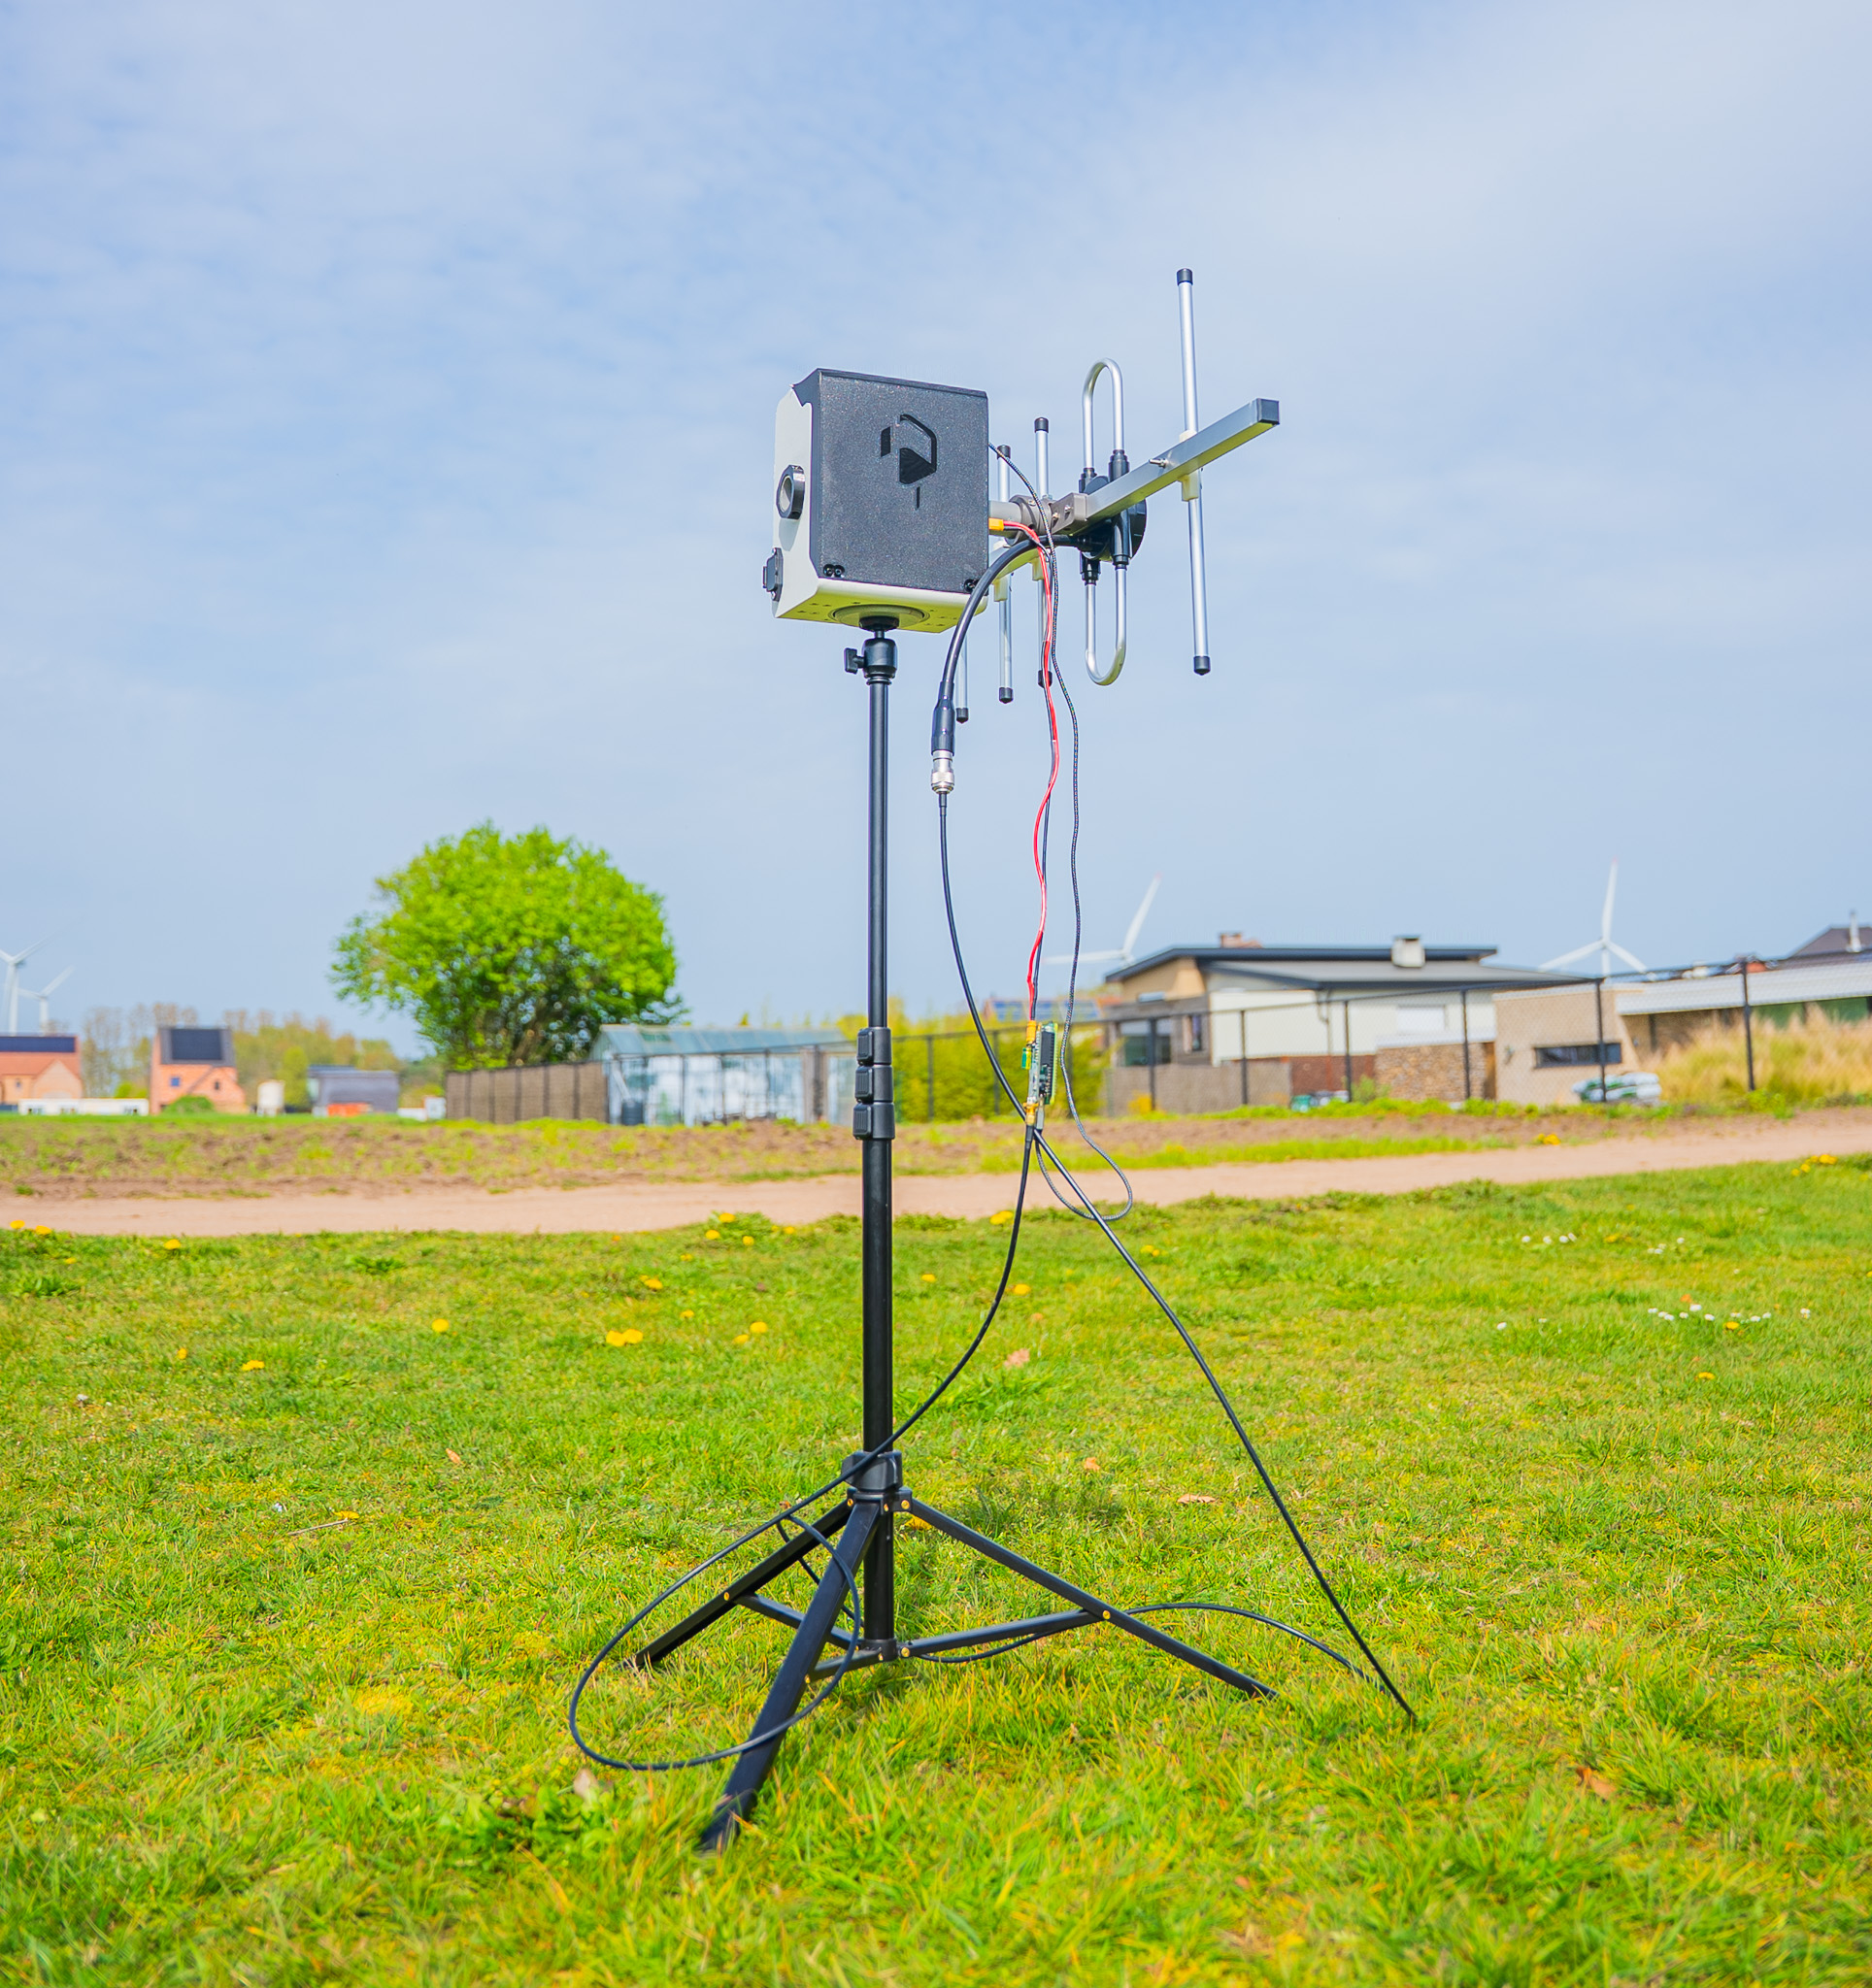
\includegraphics[width=0.85\textwidth]{photos/station_wide.jpg}
    \caption{Assembled, field-deployed ground station tracking a pass.}
\end{figure}

\paragraph{Context.}
A CubeSat is a small standardised satellite built up from 10~cm cubic units~\cite{cubesat-spec}; a 3U platform fits inside a 30$\times$10$\times$10~cm envelope, weighs a few kilograms, and can carry a meaningful scientific payload to low Earth orbit (LEO) on a rideshare launch for a fraction of the cost of a dedicated mission. KU~Leuven's AetherSpace programme is one such project, targeting a heat-shield sample-return demonstration with launch around 2030. The flight transceiver is a Texas Instruments CC1200~\cite{cc1200} on a 433~MHz UHF downlink at +14~dBm ($\approx$25~mW) into a 2~dBi turnstile or dipole antenna. Once in orbit a CubeSat is only as useful as the ground infrastructure that receives its telemetry, and providing that ground segment for AetherSpace is the subject of this thesis.

\paragraph{SatNOGS.}
The natural ecosystem to plug into is SatNOGS (Satellite Networked Open Ground Station), an open-source network of amateur ground stations that share scheduling and decoded telemetry through a public web platform. Each participating station tracks the satellites it can see, decodes the frames it captures, and uploads them to a central database; AetherSpace mission operations can then query that database without owning the receiving hardware. A station joins the network by speaking two standard interfaces: EasyComm~III over serial to the rotator and SiDS HTTP to the telemetry database. Beyond those two contracts, the choice of how to build the station is left to the operator. A full ecosystem walk-through, including the SatNOGS Network scheduler, the SDR-based receive client, and the comparison against earlier centralised projects such as GENSO, is given in the 2023 KU~Leuven masterproef by Hanssens~\cite{hanssens2023}, on which this work builds; \S\ref{sec:satnogs} summarises the parts of the ecosystem that are directly relevant to the design decisions in this thesis.

\paragraph{The gap.}
University CubeSat programmes are proliferating, but the ground-station hardware that should accompany them is not. Commercial AZ/EL rotators able to track a 433~MHz LEO link cost \euro{}760--1300~\cite{yaesu-g5500,rfham-spid}; the open-source SatNOGS v3 reference design itself still requires \euro{}300--500 in parts~\cite{satnogs-v3,satnogs-v3-bom}, and assumes a permanent rooftop installation that a student team without dedicated facilities cannot easily realise. For a project the size of AetherSpace, a fixed installation is overkill and the budget cannot justify a commercial unit.

\paragraph{This thesis.}
This work designs, builds, and field-validates a portable SatNOGS-compatible ground station that targets approximately \euro{}100 in station-core components, deploys from a standard camera tripod in about four minutes, and integrates with the SatNOGS rotator ecosystem through the standard EasyComm~III/hamlib interface. The target application is the AetherSpace mission, but neither the rotator nor the Pi-side software stack is AetherSpace-specific: any satellite present in the SatNOGS DB can be tracked, and any operator with a hamlib-compatible rotator can reuse the software.

\section{Problem Statement}
\label{sec:problem-statement}

The chapter opener established the mission (AetherSpace), the ecosystem (SatNOGS), and the gap (no cheap, portable, student-buildable station exists). This section turns those into engineering constraints. Five aspects of the problem set the design envelope: the geometry of a LEO pass, the link budget against the AetherSpace transmitter, the cost ceiling, the AetherSpace target itself, and the radio-architecture choice that follows from picking the same transceiver at both ends.

\paragraph{Geometry.}
A LEO satellite at 400~km altitude is visible from a given ground station for 5--8~minutes per 92-minute orbit. The total angular rate at zenith is bounded by
\begin{equation}
    \dot{\theta}_{\max} = \frac{v}{h} = \frac{7.67~\text{km/s}}{400~\text{km}} = 0.01918~\text{rad/s} = 1.10~\text{deg/s},
\end{equation}
with $v = \sqrt{\mu/(R_E+h)} = 7.67$~km/s for $\mu = 3.986 \times 10^{14}$~m$^3$/s$^2$ and $R_E+h = 6771$~km~\cite{montenbruck2000orbits}. For passes with closest-approach elevation above $\sim$70\degree\ the instantaneous azimuth rate exceeds 10\degree/s for a few seconds, because a small displacement of the sub-satellite point maps to a large arc in azimuth.

\paragraph{Link.}
The Siretta Oscar 44 Yagi used in this work (9~dBi peak, 54\degree$\times$48\degree\ 3-dB beamwidths at 434~MHz~\cite{siretta-oscar44}) is required to close the link against 145.8~dB of free-space path loss at 433~MHz and 30\degree\ elevation (Chapter~\ref{ch:background}, Table~\ref{tab:link-budget}). Its narrow beam sets the pointing-accuracy requirement on the rotator~\cite{stutzman2012antenna}.

\paragraph{Cost.}
Commercial rotators cost \euro{}760--900 (Yaesu G-5500~\cite{yaesu-g5500}) to \euro{}1200--1300 (SPID RAS~\cite{rfham-spid}); the SatNOGS v3 open-source rotator costs \euro{}300--500 in parts~\cite{satnogs-v3, satnogs-v3-bom}. The v2 MOTOR\_RF\_HAT BOM derived here (\S\ref{sec:cost}, design-complete) is approximately \euro{}40 for the combined controller/RF PCB, \euro{}75 for the full rotator hardware (PCB + motors + mechanics, excluding the Pi), and \euro{}100 for the station core (excluding antenna, coax, power supply, tripod).

\paragraph{Target.}
The full AetherSpace specification is given in \S\ref{sec:aetherspace}. The constraint it imposes here is link-budget closure: against a +14~dBm transmitter into a 2~dBi turnstile, the link in Chapter~\ref{ch:background} closes with positive theoretical margin only near zenith, and at 30\degree\ elevation the theoretical margin is $-5.7$~dB (Table~\ref{tab:link-budget}). Mid-elevation passes therefore demand both a directional receive antenna and a low-noise front end.

\paragraph{Radio choice.}
The station uses the CC1200 transceiver~\cite{cc1200} at both ends. This deviates from the canonical SatNOGS receive chain (SDR + GNU Radio software demodulation) but eliminates per-satellite modulation-parameter uncertainty: both ends share the same SmartRF register set once the flight configuration is finalised.

\subsection*{A deliberate alternative, not a replacement}

The canonical SatNOGS receive chain is a Raspberry Pi running the official \code{satnogs-client} daemon, an RTL-SDR v3 dongle feeding GNU Radio flowgraphs (\code{gr-satnogs}) through SoapySDR, and a hamlib-compatible rotator~\cite{satnogs-main, hamlib}. That stack decodes a broad range of amateur-satellite modulations (FSK, GFSK, AFSK, BPSK, LoRa chirp, CW, SSTV) in software, is maintained by the Libre Space Foundation, and remains the more flexible choice for a general-purpose amateur-radio ground station. The rotator produced by this thesis plugs into that stack unchanged over EasyComm III (hamlib model 204~\cite{jackson1990easycomm}).

This thesis adopts the CC1200 hardware-packet-modem path for three reasons.

The first is mission alignment. AetherSpace carries a CC1200 on-board, and using the same transceiver at the ground end eliminates modulation-parameter matching uncertainty: a single SmartRF Studio register set loaded at both ends configures identical symbol rate, deviation, filter bandwidth, sync word, and packet framing. An SDR receiver would need those values re-measured or re-derived per satellite and per flight revision.

The second is educational scope. The thesis is a joint MSc in electronics, and the CC1200 path exercises a full embedded-systems stack end-to-end: PCB design with controlled-impedance RF routing and matching networks (Chapter~\ref{ch:rf-frontend}), RP2040 firmware with SPI drivers and a binary COBS protocol (\S\ref{sec:rf-hat-firmware}, with protocol structure in Appendix~\ref{app:protocol}), Pi-side Python controlling CC1200 registers over UART (\S\ref{sec:pi-stack}), and a closed-loop tracking rotator (Chapters~\ref{ch:system-design} and~\ref{ch:firmware-software}).

The third is form-factor fit. A Pi 3A+ ships with 512~MB of LPDDR2 SDRAM~\cite{rpi3aplus}, of which approximately 416~MB is available to userspace after the default 64~MB GPU split. The SatNOGS Docker stack targets at least 1~GB of RAM~\cite{satnogs-main}; the Python stack described in \S\ref{sec:pi-stack} ($\sim$7900 LOC across the Pi packages listed in Appendix~\ref{app:bom}) runs on the 3A+ within a 200--300~MB resident-set footprint measured with \code{top}, leaving margin for the HTTPS dashboard and the systemd services.

\section{Research Questions}

The central question of this thesis is:

\begin{quote}
    Can an economical, portable SatNOGS-compatible ground station be designed, built, and field-validated as the ground segment for the AetherSpace CubeSat mission?
\end{quote}

This breaks down into six sub-questions:

\begin{enumerate}
    \item Can a satellite-tracking rotator be built for under \euro{}50 in materials?
    \item What pointing accuracy is achievable with geared DC motors, 3D-printed structure, and encoder-based PID control?
    \item Can the system integrate with the SatNOGS network using only the standard EasyComm/hamlib interface?
    \item What are the empirical trade-offs of DC motors versus stepper motors for satellite tracking?
    \item What sensitivity does the assembled CC1200 receive chain achieve in practice, and what is the dominant factor limiting it relative to the datasheet specification?
    \item Is a CC1200 hardware-modem approach a viable alternative to the SDR-based SatNOGS receive chain for the AetherSpace mission?
\end{enumerate}

\section{Scope and Division of Work}

\begin{itemize}
    \item Stan Coene: Mechanical rotator design, motor controller PCB (RP2040 + dual motor driver), rotator firmware, Raspberry Pi software stack, systemd services, web dashboard, field deployment workflow, system integration.
    \item Robbe Lehaen: RF front-end hardware (dual CC1200 transceiver HAT, UHF 433~MHz assembled + VHF 144/145~MHz routed), matching network design, Assembly of PCB's, RF HAT firmware (COBS protocol, SPI driver), CC1200 register configuration.
\end{itemize}

\section{Thesis Outline}

\begin{description}[style=unboxed, leftmargin=0pt]
    \item[Chapter~\ref{ch:background}] derives the physics of LEO satellite communication from first principles: orbital mechanics, link budgets, Doppler shift, and the SatNOGS ecosystem.
    \item[Chapter~\ref{ch:system-design}] presents the system architecture, mechanical design, rotator controller PCB, power distribution, bring-up lessons, and cost analysis.
    \item[Chapter~\ref{ch:rf-frontend}] describes the dual-CC1200 RF front-end HAT: PCB design, layout, and matching networks.
    \item[Chapter~\ref{ch:firmware-software}] covers the rotator firmware, RF HAT firmware, Raspberry Pi software stack, and field-deployment workflow.
    \item[Chapter~\ref{ch:results}] gives results and validation: tracking accuracy, RF measurements, field tests, and reception analysis. The link-budget derivation itself lives in Chapter~\ref{ch:background} and is only referenced here.
    \item[Chapter~\ref{ch:conclusion}] provides conclusions, limitations, and future work.
\end{description}

% ══════════════════════════════════════════════════════════════════════════════
\chapter{Background and Literature Review}
\label{ch:background}
% ══════════════════════════════════════════════════════════════════════════════

\section{LEO Orbital Mechanics}

\subsection{Orbital Velocity and Period}

A satellite in circular orbit at altitude $h$ orbits at radius $r = R_E + h$ ($R_E = 6371$~km). Equating gravitational and centripetal force:

\begin{equation}
    v = \sqrt{\frac{\mu}{r}}, \qquad T = 2\pi\sqrt{\frac{r^3}{\mu}}
\end{equation}

where $\mu = 3.986 \times 10^{14}$~m$^3$/s$^2$. At $h = 400$~km: $v = 7.67$~km/s, $T = 92.6$~min. The range 400--600~km covers the vast majority of CubeSat orbits, giving periods of 90--97 minutes.

\subsection{Contact Time Geometry}

% TODO: Add orbital geometry diagram (Earth, satellite orbit, ground station, slant range, visible arc, elevation angle)

The maximum slant range at the horizon ($\epsilon = 0\degree$) is:

\begin{equation}
    d_{max} = \sqrt{h^2 + 2R_E h}
\end{equation}

At 400~km: $d_{max} = 2294$~km. The visible arc subtends $\alpha = \arccos\!\left(\frac{R_E}{R_E + h}\right) = 19.6\degree$ at Earth's center, giving a maximum overhead pass duration of:

\begin{equation}
    t_{max} = \frac{2 R_E \alpha}{v} \approx 568~\text{s} \approx 9.5~\text{min}
\end{equation}

In practice, useful passes with elevation above 10\degree\ last 5--8 minutes. A single station contacts the satellite for roughly 5--10\% of its orbital period.

\subsection{Angular Velocity Across the Sky}

The satellite's angular rate as seen from the ground is slowest near the horizon and fastest near zenith. At closest approach during a zenith pass:

\begin{equation}
    \dot{\theta}_{max} = \frac{v}{h} = \frac{7672}{400 \times 10^3} = 1.1~\text{deg/s}
\end{equation}

For high-elevation passes, rates up to 2~deg/s are possible. With a 10-element Yagi ($\sim$30\degree\ 3~dB beamwidth at 434~MHz), the tracking error must stay below $\pm$15\degree\ to remain within the 3~dB beamwidth. Tracking within $\pm$5\degree\ is desirable (less than 0.3~dB loss).

% TODO: Add angular velocity plot (deg/s vs time) for a typical overhead pass

\section{The AetherSpace CubeSat}

% TODO: Add AetherSpace CubeSat render (if available from AetherSpace team)

AetherSpace is a KU Leuven project building a 3U CubeSat for a heat-shield sample return demonstration from LEO, with a planned launch around 2030. It communicates on 433~MHz UHF within the amateur satellite service allocation. The TX power is estimated at $\sim$14~dBm ($\sim$25~mW), with either a turnstile or dipole antenna ($\sim$2~dBi). Modulation and datarate are not yet finalized but will use the CC1200's native packet format.

Previous KU Leuven work: Surkijn and Van Elst (2022) studied the earth-satellite communication chain, Hanssens (2023) investigated SatNOGS ground station implementation. This thesis delivers the working ground station that those studies scoped but did not build.

% NOTE: AetherSpace team contacted for up-to-date specs (TX power, antenna, modulation, launch date).
% Update this section when confirmed.

\section{Link Budget}

The Friis transmission equation gives the received power:

\begin{equation}
    P_r = P_t + G_t + G_r - L_{fs} \quad \text{[all in dB]}
\end{equation}

where the free-space path loss is:

\begin{equation}
    L_{fs} = 20\log_{10}\!\left(\frac{4\pi d}{\lambda}\right)
\end{equation}

At 433~MHz ($\lambda = 0.693$~m), the path loss depends on the slant range $d$ between station and satellite. A \textit{zenith pass} (satellite passes directly overhead, elevation = 90\degree) has the shortest slant range, equal to the orbital altitude. A \textit{mid-elevation pass} (peak elevation $\sim$30--50\degree) is the most common useful geometry. At the \textit{horizon} (elevation = 0\degree), the slant range is at its maximum.

\begin{table}[H]
    \centering
    \begin{tabular}{lccc}
        \toprule
        Scenario & Peak elevation & Slant range & $L_{fs}$ \\
        \midrule
        Zenith pass & 90\degree & 400~km & 137.2~dB \\
        Mid-elevation & $\sim$40\degree & 600~km & 140.7~dB \\
        Horizon & 0\degree & 2294~km & 152.4~dB \\
        \bottomrule
    \end{tabular}
    \caption{Free-space path loss at 433~MHz for different pass geometries.}
    \label{tab:path-loss}
\end{table}

Table~\ref{tab:link-budget} shows the full link budget for a mid-elevation pass at 600~km slant range.

\begin{table}[H]
    \centering
    \begin{tabularx}{\textwidth}{lr>{\raggedright\arraybackslash}X}
        \toprule
        Parameter & Value & Notes \\
        \midrule
        TX power (CubeSat) & +14~dBm & $\sim$25~mW (AetherSpace estimate) \\
        TX antenna gain & +2~dBi & Turnstile or dipole \\
        Free-space path loss & $-$140.7~dB & 600~km, 433~MHz \\
        Atmospheric loss & $-$1~dB & Ionospheric + tropospheric attenuation; negligible at zenith, up to 1~dB at low elevations \\
        Polarization mismatch & $-$3~dB & CubeSat tumbles in orbit, randomizing polarization relative to the linearly-polarized Yagi; 3~dB average loss \\
        RX antenna gain (Yagi) & +10~dBi & 10-element at 434~MHz \\
        \midrule
        \textbf{Received power} & \textbf{$-$118.7~dBm} & \\
        CC1200 sensitivity & $-$120~dBm & At 2.4~kbps \\
        \textbf{Link margin} & \textbf{1.3~dB} & \\
        \bottomrule
    \end{tabularx}
    \caption{Link budget for AetherSpace UHF downlink at 433~MHz.}
    \label{tab:link-budget}
\end{table}

With only 1.3~dB of margin at 600~km, the link is tight. At zenith ($d = 400$~km, $L_{fs} = 137.2$~dB), the margin improves to 4.8~dB. At the horizon ($d = 2294$~km, $L_{fs} = 152.4$~dB), the margin is $-$10.4~dB---the link does not close. Communication is only viable above $\sim$20\degree\ elevation with 14~dBm TX power. Reducing the datarate below 2.4~kbps would improve CC1200 sensitivity and widen the margin. Accurate antenna pointing becomes critical: even a few degrees of pointing error costs dB that cannot be spared.

\section{Doppler Shift}

A satellite moving with radial velocity $v_r$ relative to the ground station shifts the received frequency by:

\begin{equation}
    \Delta f = \frac{v_r}{c} \cdot f_0
\end{equation}

The maximum radial velocity occurs at the horizon, where the orbital velocity projects fully onto the line of sight: $v_{r,max} \approx 7229$~m/s. This gives:

\begin{itemize}
    \item At 433~MHz (UHF): $\Delta f_{max} = \pm 10.4$~kHz
    \item At 145.9~MHz (VHF): $\Delta f_{max} = \pm 3.5$~kHz
\end{itemize}

These shifts are significant relative to the CC1200's receive bandwidth of $\sim$30~kHz at 2.4~kbps. Without compensation, the signal drifts out of the passband within seconds. Our station software updates the CC1200 frequency registers at 2~Hz, limiting the uncompensated drift between updates to $\sim$106~Hz---well within the receiver bandwidth.

% TODO: Add Doppler shift vs time plot for a typical pass

\section{The SatNOGS Network}

SatNOGS (Satellite Networked Open Ground Station) started at Hackerspace.gr in Athens during the 2014 NASA Space Apps Challenge, winning the Hackaday Prize which funded the Libre Space Foundation. As of 2025: over 400 active stations, 50+ countries, 1177+ tracked satellites, 165+ million data frames.

The ecosystem has four parts:

\begin{description}
    \item[SatNOGS Network] (network.satnogs.org) --- schedules observations across stations based on pass predictions, collects results.
    \item[SatNOGS DB] (db.satnogs.org) --- decoded telemetry database, supports the SiDS (Simple Downlink Sharing) protocol.
    \item[SatNOGS Client] --- Python daemon on each station. Gets observation jobs, controls the rotator via hamlib/rotctld, controls the receiver (typically RTL-SDR via SoapySDR/GNU Radio), uploads results.
    \item[SatNOGS Rotator] --- optional open-source rotator (3D-printed, NEMA17 steppers, Arduino controller).
\end{description}

Rotator communication goes through \textbf{hamlib}, an open-source library for amateur radio equipment. The \code{rotctld} daemon exposes a TCP interface (port 4533) accepting EasyComm commands. Any controller that speaks EasyComm over serial works with SatNOGS without modification.

\subsection{The EasyComm Protocol}

EasyComm is an ASCII protocol developed by Patrik Linder (SM0TQX) for antenna tracking. The SatNOGS variant (hamlib model 204) uses:

\begin{table}[H]
    \centering
    \begin{tabular}{ll}
        \toprule
        Command & Function \\
        \midrule
        \code{AZxxx.x ELyyy.y} & Set target azimuth and elevation \\
        \code{AZ} / \code{EL} & Query current position \\
        \code{VE} & Query firmware version \\
        \code{GS} & Get status (0 = idle, 1 = moving) \\
        \code{GE} & Get error flags \\
        \code{SA} / \code{SE} / \code{STOP} & Stop azimuth / elevation / both \\
        \code{RESET} & Home the rotator \\
        \code{PARK} & Move to park position (0\degree, 0\degree) \\
        \bottomrule
    \end{tabular}
    \caption{EasyComm command set (SatNOGS variant).}
    \label{tab:easycomm}
\end{table}

Each command is a newline-terminated ASCII string. No binary framing, no handshaking. The entire parser fits in $\sim$50 lines of C.

\subsection{Why a Distributed Network}

A single station contacts a LEO satellite for at most $\sim$10\% of each orbit. For mission-critical telemetry this is not enough. SatNOGS solves this by distributing stations worldwide so nearly every orbit has coverage. Previous attempts (Mercury GSN, Japanese GSN, ESA's GENSO) failed because they required homogeneous hardware. SatNOGS accepts any hardware that speaks EasyComm and uses an SDR receiver.

\section{Existing Ground Station Designs}

\begin{table}[H]
    \centering
    \begin{tabularx}{\textwidth}{llcl>{\raggedright\arraybackslash}X}
        \toprule
        System & Type & Cost (EUR) & Accuracy & Notes \\
        \midrule
        Yaesu G-5500 & Commercial & 900--1200 & $\sim$1\degree & Industry standard, heavy, needs separate controller \\
        SPID RAS & Commercial & 400--800 & $\sim$1\degree & Lighter alternative \\
        Alfa Radio RAS & Commercial & 500--700 & $\sim$1\degree & Similar to SPID \\
        SatNOGS v3 & Open-source & 150--300 & $\sim$1\degree & 3D-printed, NEMA17 steppers, belt drive \\
        SQ3SWF & Open-source & $\sim$100 & $\sim$2\degree & Compact 3D-printed stepper design \\
        \textbf{This work} & \textbf{Open-source} & \textbf{$<$50} & \textbf{$<$0.3\degree} & \textbf{ASA 3D-printed, geared DC motors, EasyComm} \\
        \bottomrule
    \end{tabularx}
    \caption{Cost comparison of satellite tracking rotator systems.}
    \label{tab:rotator-comparison}
\end{table}

\subsection{The SatNOGS v3 Rotator}

The official SatNOGS rotator uses two NEMA17 bipolar steppers with GT2 belt reduction, controlled by an Arduino MEGA with CNC shield and A4988 drivers. BOM: EUR~150--300. Known limitations:

\begin{itemize}
    \item Steppers draw 0.5--1.0~A holding current even when stationary---bad for battery operation.
    \item Low belt-drive gear ratio requires microstepping for smooth tracking, which reduces torque.
    \item Assembly needs precise belt tensioning and shaft alignment.
\end{itemize}

\subsection{University Implementations}

Most university ground stations (UPSat/Patras, TU Delft/Delfi-C3, AraMiS/Politecnico di Torino) buy commercial rotators and focus on RF or software. Few attempt custom mechanical design. DIY exceptions: EA4GPZ's servo-based portable rotator, the Open Rotator Project (DC motors with potentiometer feedback), and SuperAntennaz for heavy loads.

\subsection{Comparison with Hanssens (2023)}

This thesis builds on Hanssens' 2023 study, which surveyed SatNOGS, assessed antenna options, and tested a Stepperdrive MSD-50-5.6D stepper motor. His work identified that the stepper-and-belt approach required more torque than available for reliable azimuth rotation under wind loading. This informed our choice of high-torque geared DC motors with a higher gear ratio.

\begin{table}[H]
    \centering
    \begin{tabularx}{\textwidth}{l>{\raggedright\arraybackslash}X>{\raggedright\arraybackslash}X}
        \toprule
        Aspect & Hanssens (2023) & This work (2026) \\
        \midrule
        Rotator & Preliminary stepper test & Fully built ASA 3D-printed rotator \\
        Motor control & Not implemented & Custom PCB: dual TB6642FG + RP2040 \\
        Firmware & Not implemented & EasyComm firmware with PID control \\
        Pi integration & Theoretical description & Python stack ($\sim$4000 LOC) + web dashboard \\
        RF front-end & Not implemented & Dual CC1200 HAT (UHF + VHF) \\
        Field deployment & Not addressed & Zero-SSH smartphone workflow \\
        Cost analysis & Not performed & Full BOM, $<$EUR~50 rotator \\
        Tracking & Not demonstrated & Live tracking validated ($<$0.3\degree\ error) \\
        \bottomrule
    \end{tabularx}
    \caption{Advancement over Hanssens (2023).}
    \label{tab:hanssens-comparison}
\end{table}

Our design combines: (a) 3D-printed deep groove ball bearings integrated into the chassis, (b) 516:1 internally geared DC motors with zero idle current, and (c) full SatNOGS compatibility via EasyComm, verified with live satellite passes.

% ══════════════════════════════════════════════════════════════════════════════
\chapter{System Design}
\label{ch:system-design}
% ══════════════════════════════════════════════════════════════════════════════

\section{System Architecture}

The station is built around a Raspberry Pi 3A+ that bridges three independent subsystems: a 2-axis AZ/EL rotator that aims a directional antenna at the satellite, an RF front-end that demodulates the signal received through that antenna, and a Python software stack that decides where to point and what to listen for. Figure~\ref{fig:system-arch} shows the data and power flow across the whole station; the rest of this section walks through it block by block.

\begin{figure}[H]
    \centering
    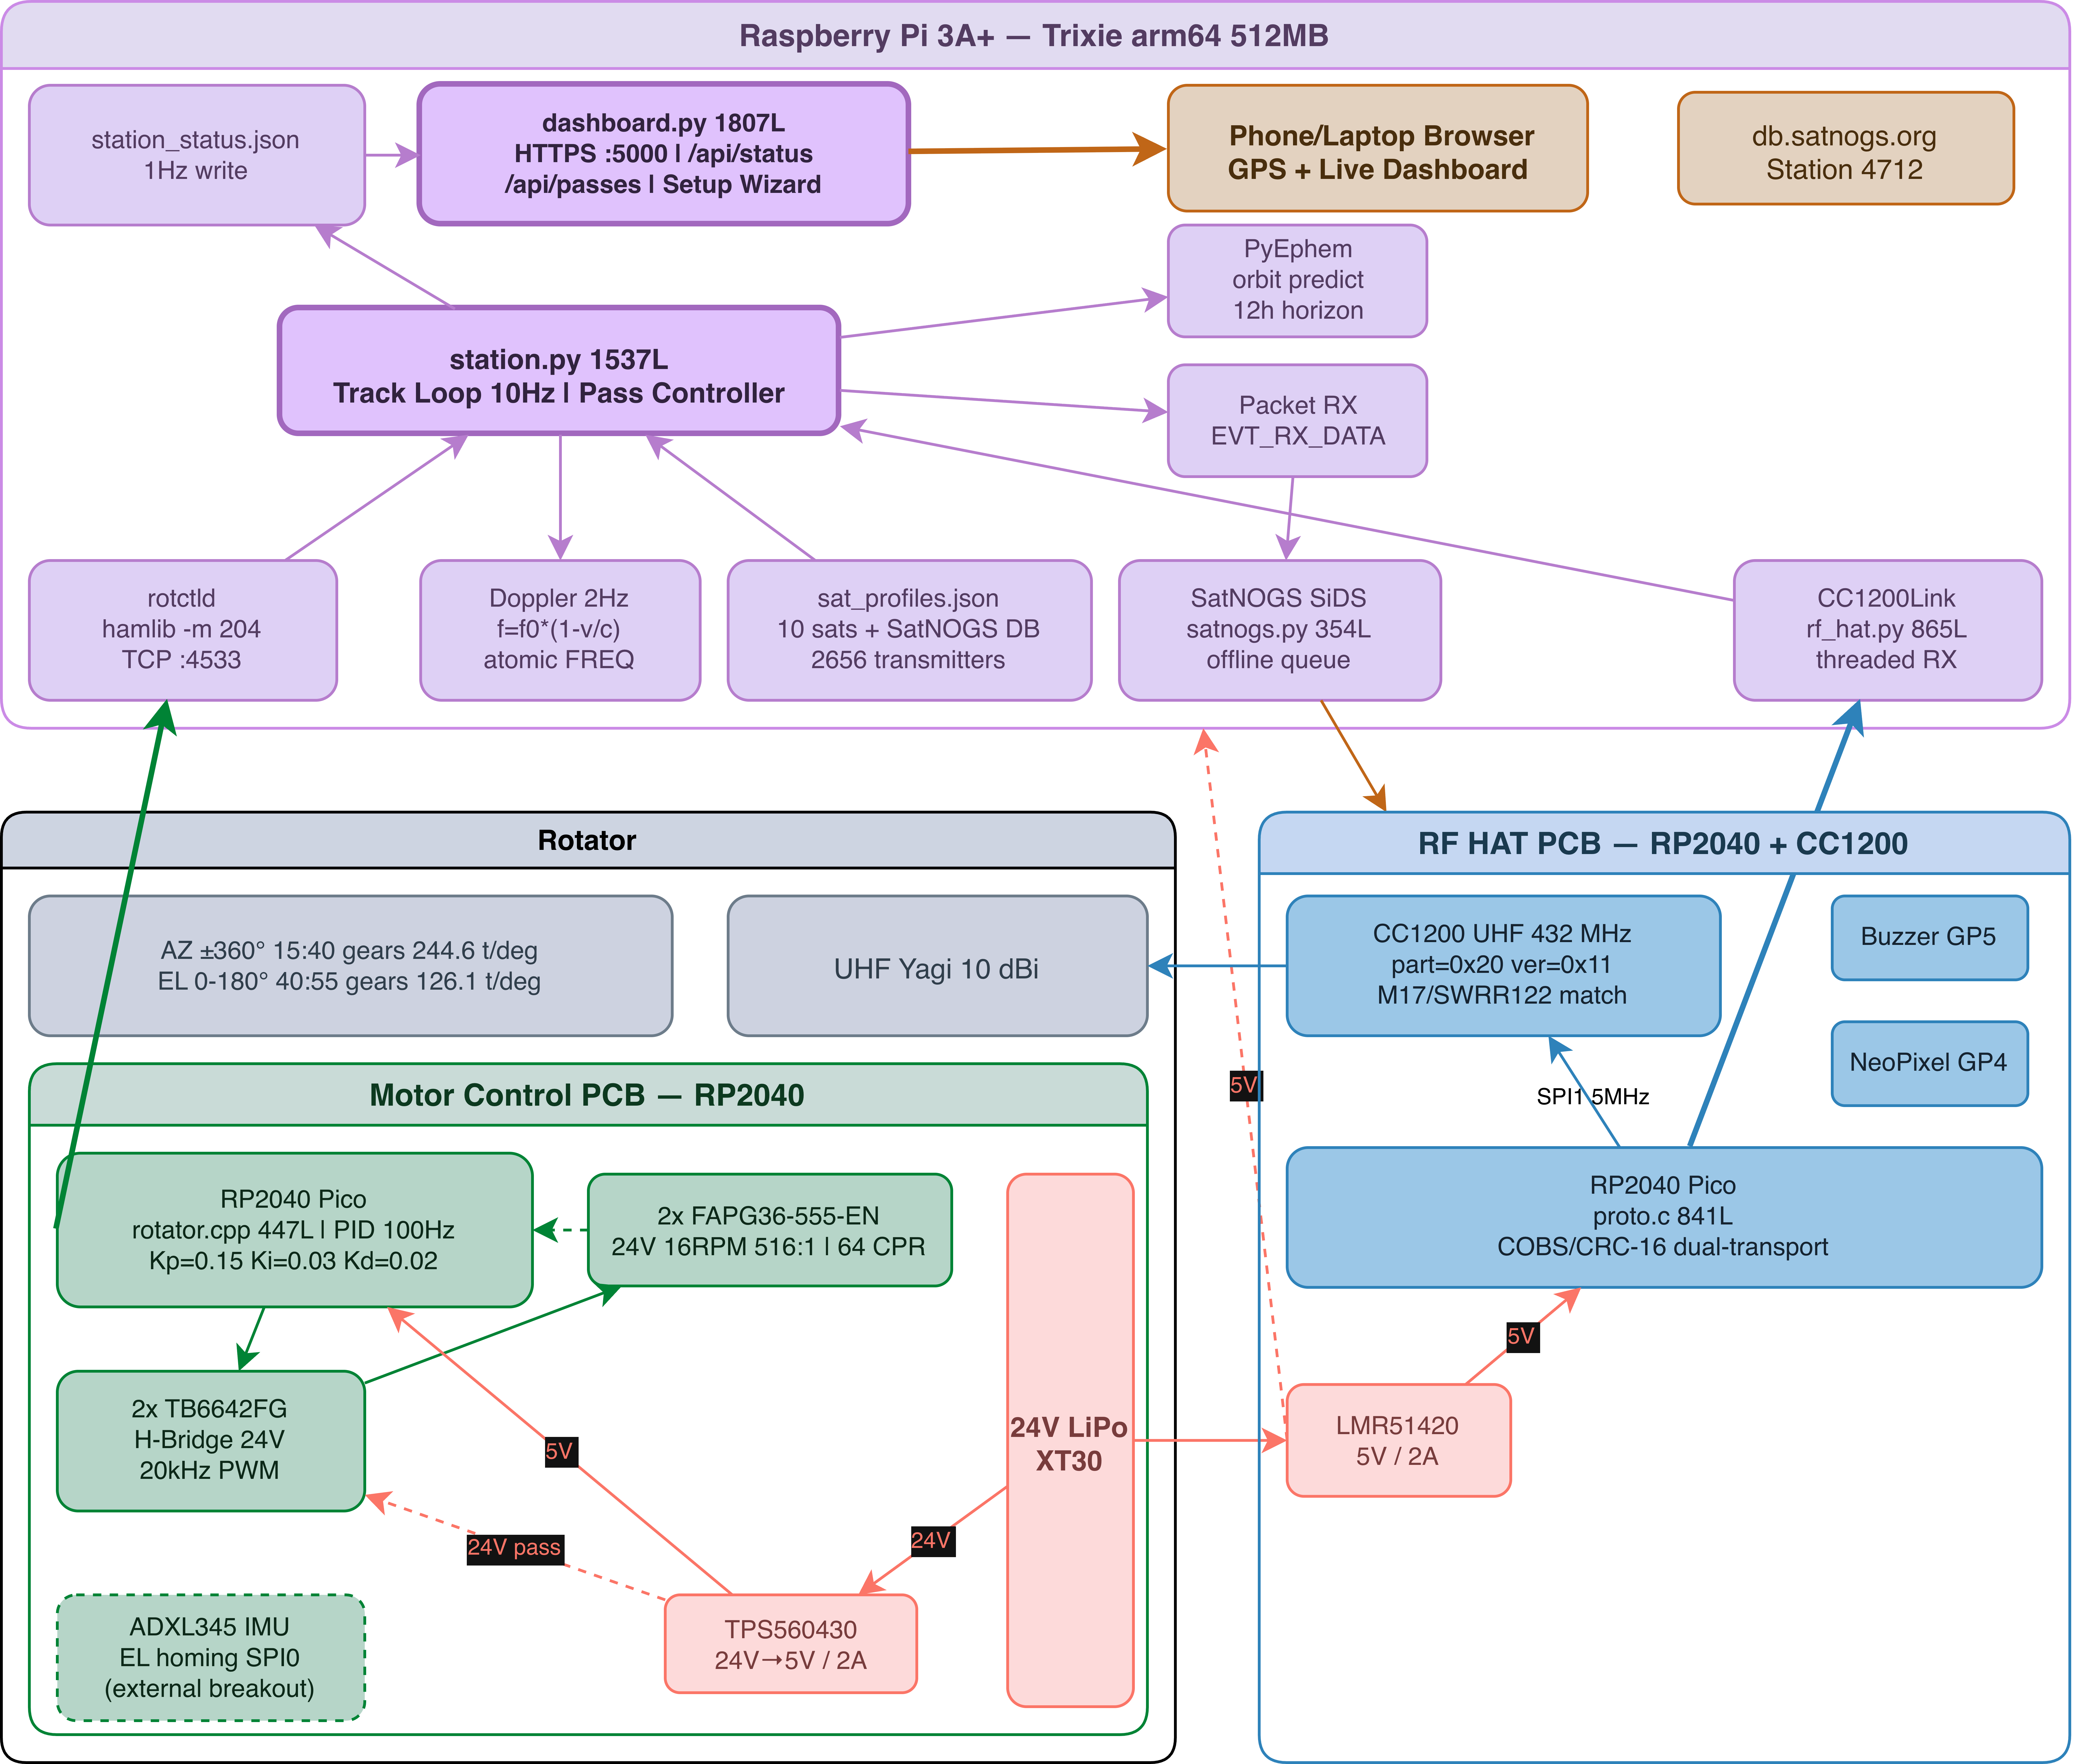
\includegraphics[width=\textwidth]{figures/system_architecture.png}
    \caption{Station architecture: Pi 3A+ host, MotorPCB, dual-CC1200 RF HAT, and power tree.}
    \label{fig:system-arch}
\end{figure}

\paragraph{Antenna chain.}
The AetherSpace CubeSat radiates a 433~MHz CC1200 downlink which, after $\sim$1000~km of free-space path, arrives at a directional UHF Yagi (Siretta Oscar 44, 9~dBi) bolted to the elevation cradle of the rotator. The Yagi feeds the RF HAT through a 3~m RG58 coax run terminated at an SMA connector on the HAT. The dashed link from the satellite to the antenna in Figure~\ref{fig:system-arch} marks this path as the link budget of \S\ref{sec:link-budget}.

\paragraph{RF HAT.}
A Raspberry Pi HAT carries the receive electronics: a CC1200 sub-GHz transceiver on a controlled-impedance RF section (with a second CC1200 footprint routed for VHF but not populated on the v1 board), a 5~V LMR51420 buck converter, a Raspberry Pi Pico (RP2040) acting as the radio's local controller, and two operator-feedback peripherals on the RP2040 GPIO (a piezo buzzer for AOS/LOS/error patterns and four WS2812B NeoPixels for status colour). The CC1200 talks to the RP2040 over a 5~MHz SPI1 bus; the RP2040 in turn frames a binary COBS protocol with CRC-16/CCITT-FALSE and pushes it to the Pi through the dedicated UART on \file{/dev/serial0}. Chapter~\ref{ch:rf-frontend} covers the RF schematic, layout, and matching network in detail.

\paragraph{Motor controller PCB.}
A second RP2040 (also on a Pi Pico module) runs the closed-loop tracking firmware: it reads two FAPG36-555-EN brushed DC gearmotors over their built-in quadrature encoders (64~CPR after 4$\times$ decode), drives them through two TB6642FG H-bridges at 20~kHz PWM, and exposes the standard EasyComm~III serial protocol to the Pi through USB CDC. An external ADXL345 IMU breakout provides the gravity vector for elevation homing at boot (SPI0). The 24~V supply that feeds the H-bridges is also stepped down on-board by a TPS560430 5~V/2~A buck for the Pico's logic rail. The two-axis output drives the AZ ($\pm$360\degree, 15:40 external reduction, 244.6 ticks/\degree) and EL (0--180\degree, 40:55 external reduction, 126.1 ticks/\degree) gear trains of the 3D-printed rotator described in \S\ref{sec:motors} and \S\ref{sec:gearing}.

\paragraph{Station computer.}
The Raspberry Pi 3A+ runs Debian Trixie (armhf, 512~MB) and hosts the application stack. \code{rotctld} from the hamlib package translates the rotator-side TCP control protocol on port~4533 into EasyComm~III bytes on the USB CDC link to the motor PCB. \code{station.py}, the tracking daemon, owns the orbital state machine, runs PyEphem at 10~Hz to compute commanded AZ/EL and Doppler-corrected frequency, drives \code{rotctld} and the RF HAT in lockstep, and emits a 1~Hz status snapshot at \file{\textasciitilde/.station\_status.json}. \code{dashboard.py} reads that snapshot and serves a self-signed HTTPS dashboard on port~5000 to a phone or laptop browser. \code{satnogs.py} pushes CRC-valid frames to the SatNOGS DB (station ID 4712) over the SiDS HTTP API, with an offline queue for sessions without internet. PyEphem is fed by TLE data periodically refreshed from AMSAT and CelesTrak, and per-satellite radio profiles come from a hand-curated \file{sat\_profiles.json} with a SatNOGS DB transmitter-API fallback. Chapter~\ref{ch:firmware-software} expands the Pi stack.

\paragraph{External services and operator.}
Three external hosts close the loop. AMSAT and CelesTrak supply orbital elements (TLEs) over plain HTTP; SatNOGS DB receives decoded telemetry over HTTPS. The operator's phone or laptop browser connects to the Pi's HTTPS dashboard for setup, GPS entry, and live monitoring; SSH is not used in the deployment workflow.

\paragraph{Power tree.}
A single 24~V bench supply (or 6S LiPo for portable operation) feeds the motor PCB's 24~V H-bridge rail directly and is dropped to 5~V on each board independently: an LMR51420 on the RF HAT and a TPS560430 on the motor PCB. The 5~V rail of the RF HAT also supplies the Pi through the GPIO header. Splitting the buck converters this way prevents the high-current H-bridge switching transients on the motor PCB from propagating into the RF HAT's 5~V rail; each board's switching regulator is local to its own load.

\paragraph{Boot order.}
Five systemd units start the station autonomously after the Pi finishes booting: \code{rfkill-unblock} clears the default-blocked WiFi on Trixie, \code{wifi-provision} hosts a captive-portal SSID/password entry if no WiFi is configured, \code{rotctld} starts the hamlib daemon, \code{dashboard} starts the HTTPS server, and \code{station} starts the tracking daemon once \file{station.conf} (written by the dashboard's setup wizard from the operator's phone GPS) is available.

\paragraph{Subsystem independence.}
The architecture deliberately keeps rotator and RF independent: each subsystem has its own RP2040 and its own protocol to the Pi (USB CDC EasyComm vs.\ UART COBS), so either side can be tested, replaced, or upgraded in isolation. The v2 MOTOR\_RF\_HAT collapses both PCBs onto a single 6-layer Pi HAT (\S\ref{sec:cost}), but the firmware boundary stays the same: the merged board still presents two logically distinct devices to the Pi.

\paragraph{Design constraints.}
Four constraints shape the architecture. Portability is enforced by a 1/4"-20 UNC tripod thread on the base, with the full setup measured at approximately 4 minutes from unpacking to first tracked pass across three field sessions (\S\ref{sec:field-tests}). The zero-SSH workflow routes every field operation, GPS entry, north alignment, pass selection, park, and shutdown, through the HTTPS dashboard, which targets a laptop browser but also works on a phone for quick tasks such as supplying a GPS fix. The cost target is the v2 MOTOR\_RF\_HAT BOM derived in \S\ref{sec:cost} and listed in Appendix~\ref{app:bom}: $\sim$€40 for the combined controller/RF PCB, $\sim$€75 for the rotator hardware, $\sim$€100 for the station core (excluding antenna, coax, power supply, tripod). The intended licensing is CERN-OHL-S v2 for hardware and MIT for firmware and Python stack, with the formal \file{LICENSE} files added on the open-source release.

\section{Mechanical Design}

The rotator is designed in Onshape and printable on consumer FDM machines with a 220$\times$220~mm bed (the largest single printed part is 205$\times$160$\times$120~mm). All structural prints are in ASA (Acrylonitrile Styrene Acrylate), an outdoor-grade engineering filament for desktop FDM. ASA is chosen over PLA for two properties: (i) UV stability from the acrylate rubber phase (a polymer-science property of ASA copolymers; ASA substitutes the acrylate rubber for the butadiene phase of ABS, eliminating the UV-degradation vector), and (ii) a glass transition $T_g \approx 100$\degC / Vicat softening $\approx$~105\degC, compared to $T_g \approx 60$\degC\ for PLA; this margin avoids thermal deformation in direct sunlight. PETG was considered and rejected because of lower interlayer adhesion and creep under sustained load compared with ASA at equivalent print settings.

\begin{figure}[H]
    \centering
    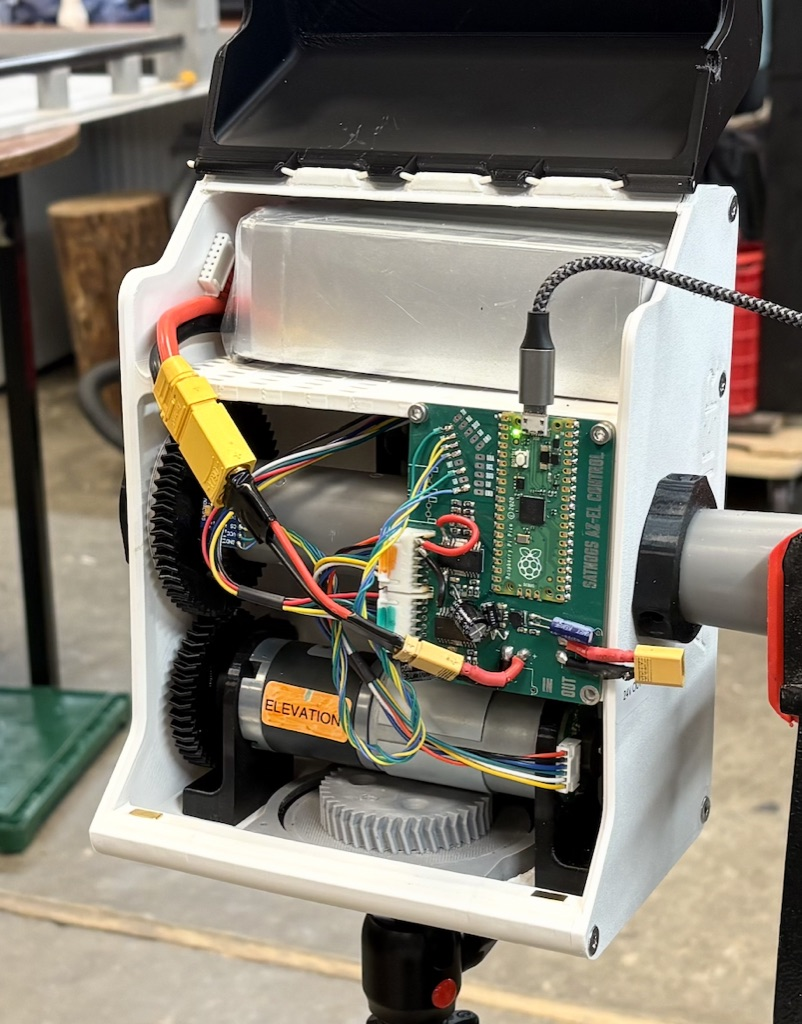
\includegraphics[width=0.7\textwidth]{photos/rotator_hero_2.jpg}
    \caption{Assembled 3D-printed rotator, front view.}
\end{figure}

\subsection{Structure}

The chassis consists of a base plate with an integrated azimuth bearing race, two side plates forming the elevation frame, and a removable hood covering the electronics compartment. The hood attaches via a 3D-printed hinge, giving tool-free access to cable connections during bring-up.

The station mounts to any standard camera tripod through a 1/4"-20 UNC brass heat-set insert in the base plate. Using the tripod standard rather than a custom mount lets the station share hardware with existing camera tripods in the user's toolkit.

The elevation axis is a PVC pipe passing through both side plates. The elevation gear is clamped directly onto this pipe by integrated 3D-printed screw clamps. The clamp geometry lets the EL gear be slid along the pipe during assembly to set mesh with the motor pinion, without set screws or adhesives.

All fasteners are M4$\times$10~mm countersunk screws for structural joints and M3$\times$8~mm for motor mounts. The assembly uses no adhesives (every joint is either a press-fit, a screw fastener, or a clamp), so the station disassembles for transport or repair without destructive separation.

\subsection{Bearings}

Both axes use 3D-printed deep-groove ball bearings with COTS 3~mm steel balls. The elevation outer race is printed in place into the side plate. The azimuth outer race is a separate screw-in part: the raceway has to be printed flat-down on the build plate to avoid layer stairstepping on the running surface, which prevents printing it as a feature of the base plate. Inner races are separate rings that double as the rotating element (the main disk for AZ); a press-in 3D-printed retainer holds the ball complement.

The trade-off is surface finish: printed races have higher $R_a$ than machined steel bearings. Two properties of the rotator keep this acceptable: (i) the operating speed at the output is bounded by the motor output divided by the external ratio (approximately 6~RPM on the AZ axis via the 15:40 reduction, approximately 11~RPM on EL via the 40:55 reduction, at 95\,\% duty; \S\ref{sec:slew-speed}), so contact-surface sliding velocity is low; and (ii) the bearing preload is low because the herringbone gear pair below imposes negligible axial thrust load (\S\ref{sec:gearing}). Endurance characterisation beyond the field sessions is future work.

\begin{figure}[H]
    \centering
    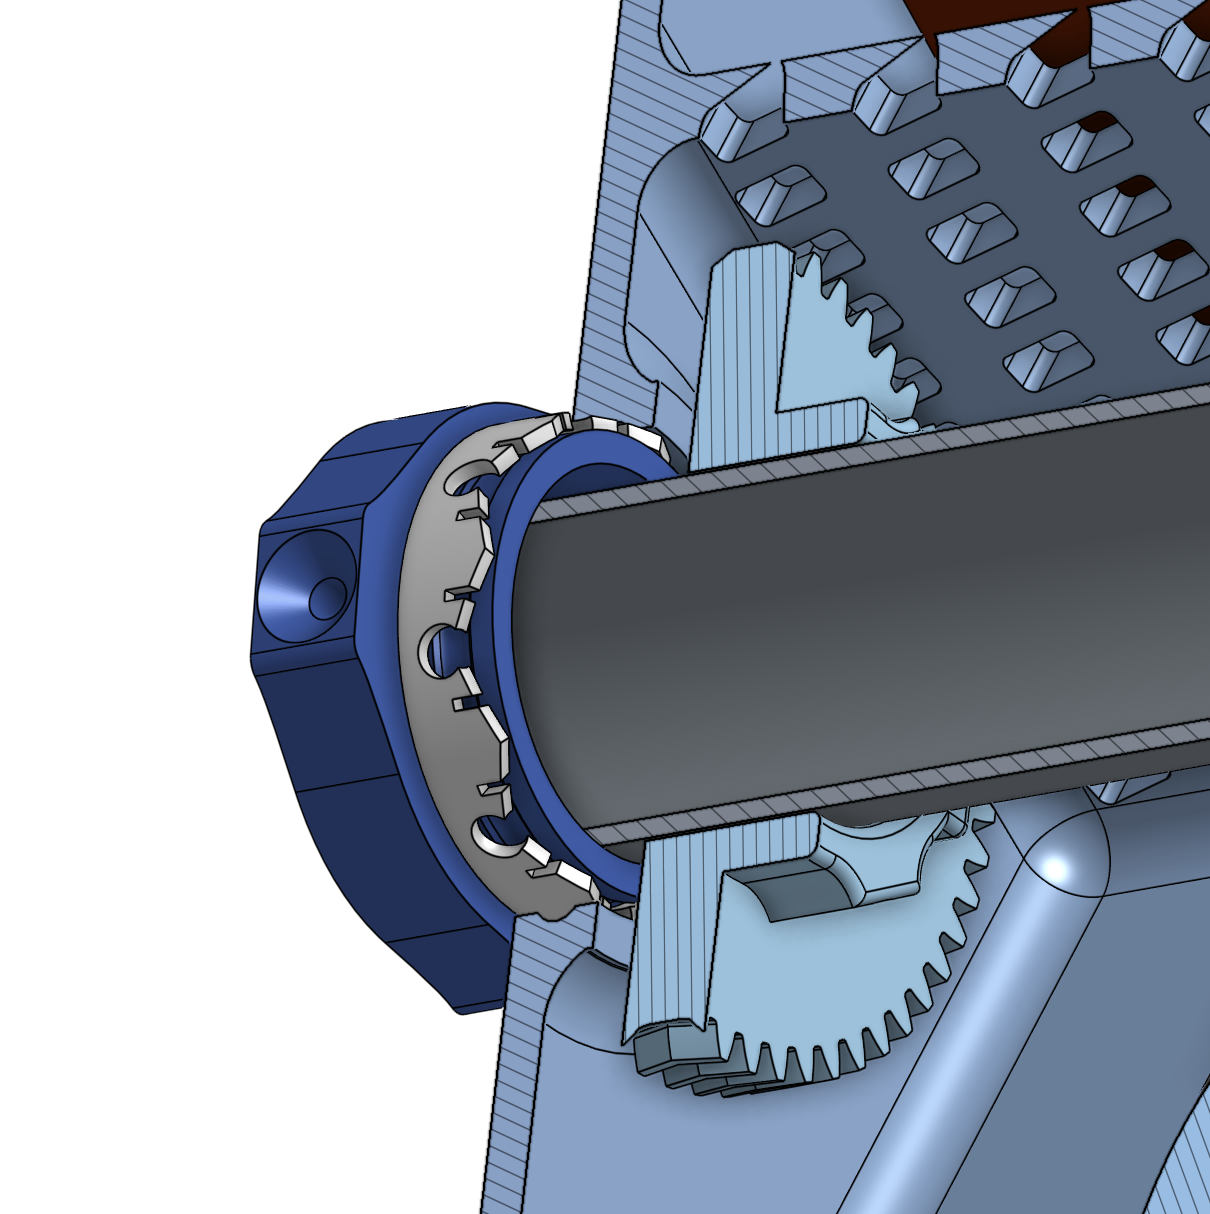
\includegraphics[width=0.6\textwidth]{photos/3DP_bearings_close-up.png}
    \caption{3D-printed deep-groove ball bearing close-up with 3\,mm steel balls and press-in retainer.}
\end{figure}

\begin{figure}[H]
    \centering
    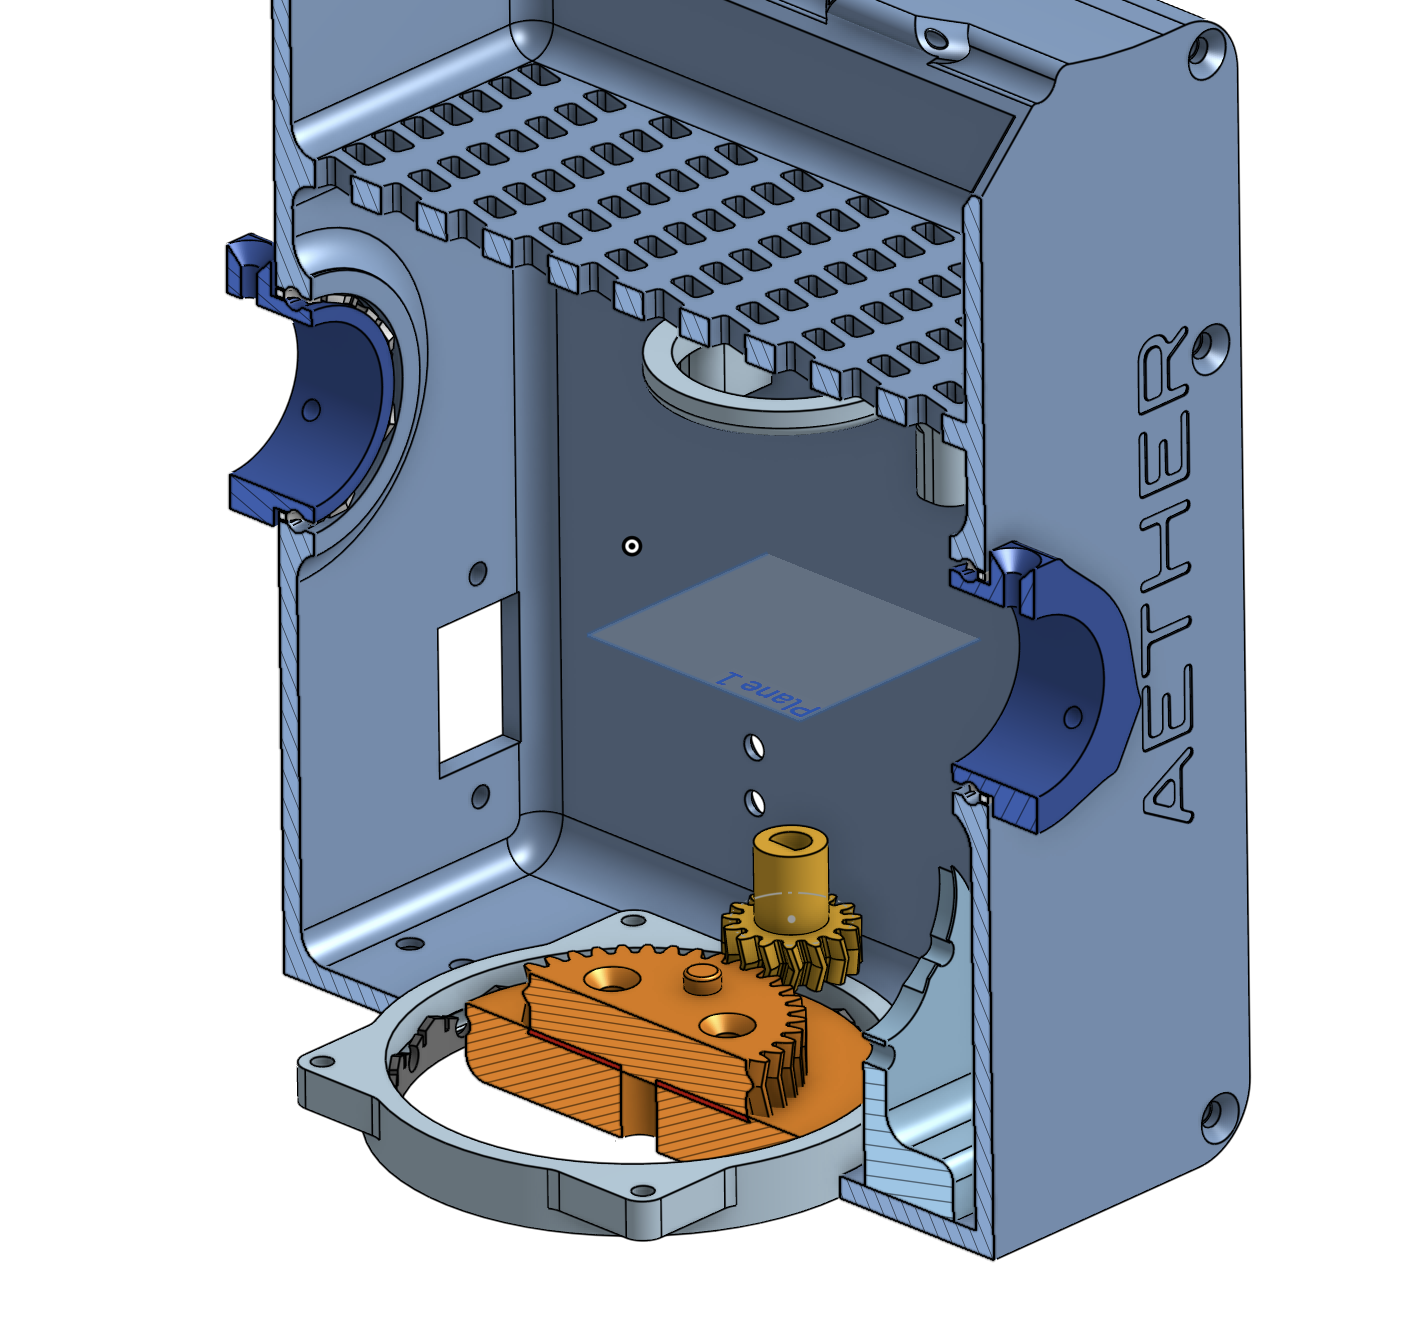
\includegraphics[width=0.7\textwidth]{photos/3DP_bearings_all.png}
    \caption{Both printed bearings assembled, with the separate AZ inner race printed flat-down.}
\end{figure}

\subsection{Gearing}
\label{sec:gearing}

All gears use a double-helical (herringbone) tooth profile with a 15\degree\ helix angle, 4/3~mm normal module, and 8~mm face width. The herringbone profile cancels the axial thrust generated by each helical half on a single-helical gear, which matters here because the printed radial deep-groove bearings tolerate much less axial than radial load. The 4/3~mm module is non-standard in the ISO 53 preferred series~\cite{iso53} but gives integer reference diameters (e.g. 15 teeth $\times$ 4/3~mm = 20~mm) that print cleanly on FDM at 0.2~mm layer height.

The gear-ratio bookkeeping:

\begin{table}[H]
    \centering
    \footnotesize
    \begin{tabular}{@{}lllllllc@{}}
        \toprule
        Axis & Teeth & Ext. ratio & Internal gearbox & Total ratio & CPR & Ticks/\degree & Travel \\
        \midrule
        AZ & 15:40 & 2.667:1 & 516:1 & 1376:1  & 64 & 244.6 & $\pm$360\degree \\
        EL & 40:55 & 1.375:1 & 516:1 & 709.5:1 & 64 & 126.1 & 0--180\degree \\
        \bottomrule
    \end{tabular}
    \caption{Rotator gear ratios, encoder counts, and per-axis positional resolution.}
\end{table}

Ticks per degree at the output is derived from the encoder count per motor revolution multiplied by the total reduction, divided by 360:

\begin{itemize}
    \item AZ: $\text{ticks/deg} = \dfrac{64 \times 516 \times (40/15)}{360} = \dfrac{64 \times 516 \times 2.667}{360} = \dfrac{88\,064}{360} = 244.6$ ticks/deg, giving a positioning resolution of $1/244.6 = 0.00409\degree$ per tick.
    \item EL: $\text{ticks/deg} = \dfrac{64 \times 516 \times (55/40)}{360} = \dfrac{64 \times 516 \times 1.375}{360} = \dfrac{45\,408}{360} = 126.1$ ticks/deg, giving 0.00793\degree\ per tick.
\end{itemize}

Gears press-fit directly onto the motor's 6~mm D-shafts with additional set-screws.

\begin{figure}[H]
    \centering
    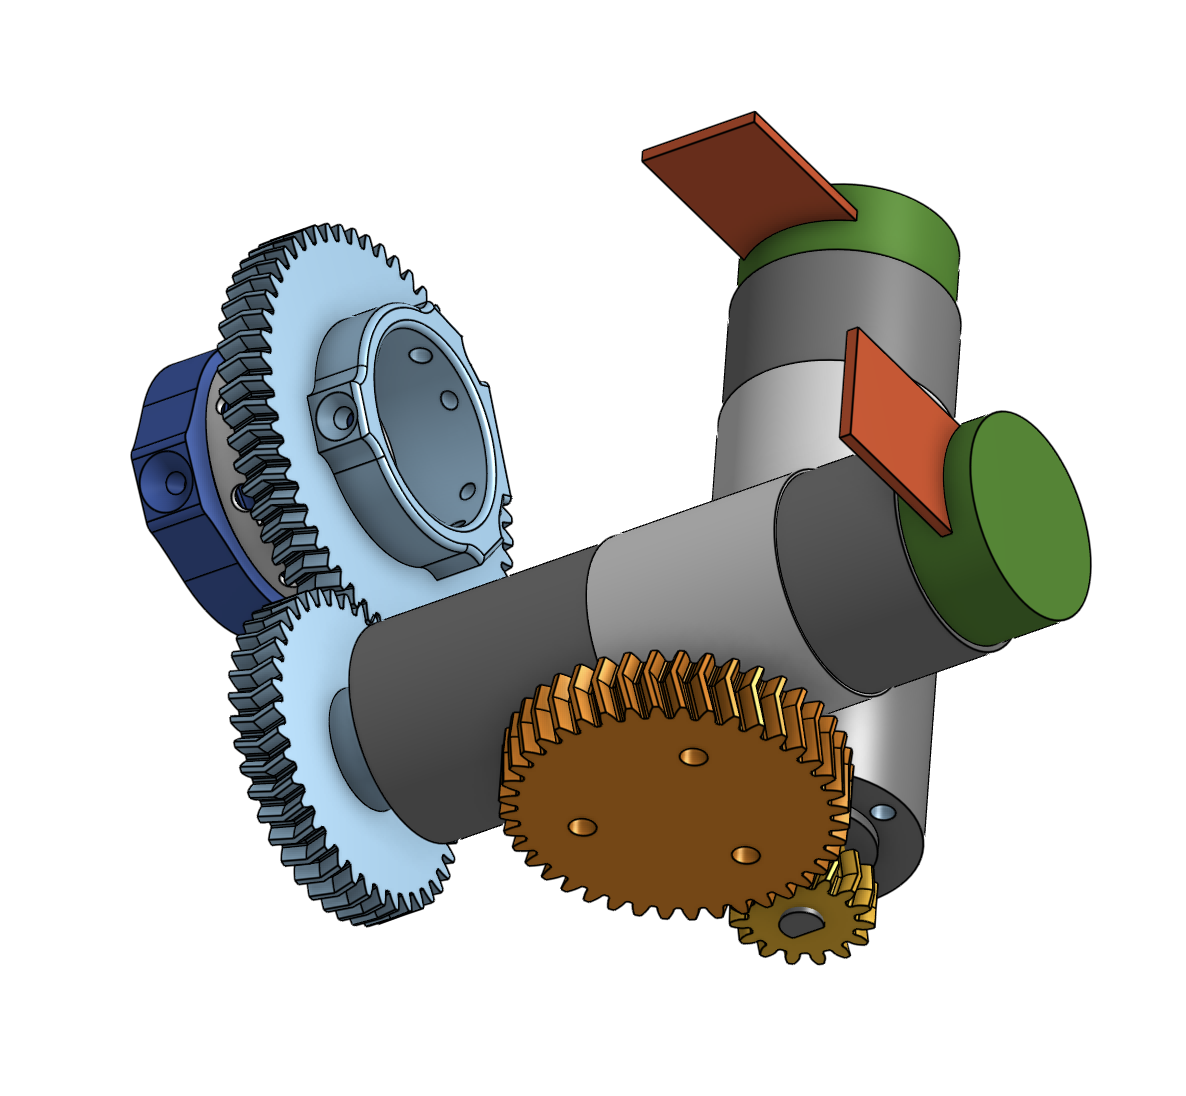
\includegraphics[width=0.7\textwidth]{photos/3DP_gears_all.png}
    \caption{Printed herringbone gear set: AZ pair (15:40, 2.667:1) and EL pair (40:55, 1.375:1).}
\end{figure}

\begin{figure}[H]
    \centering
    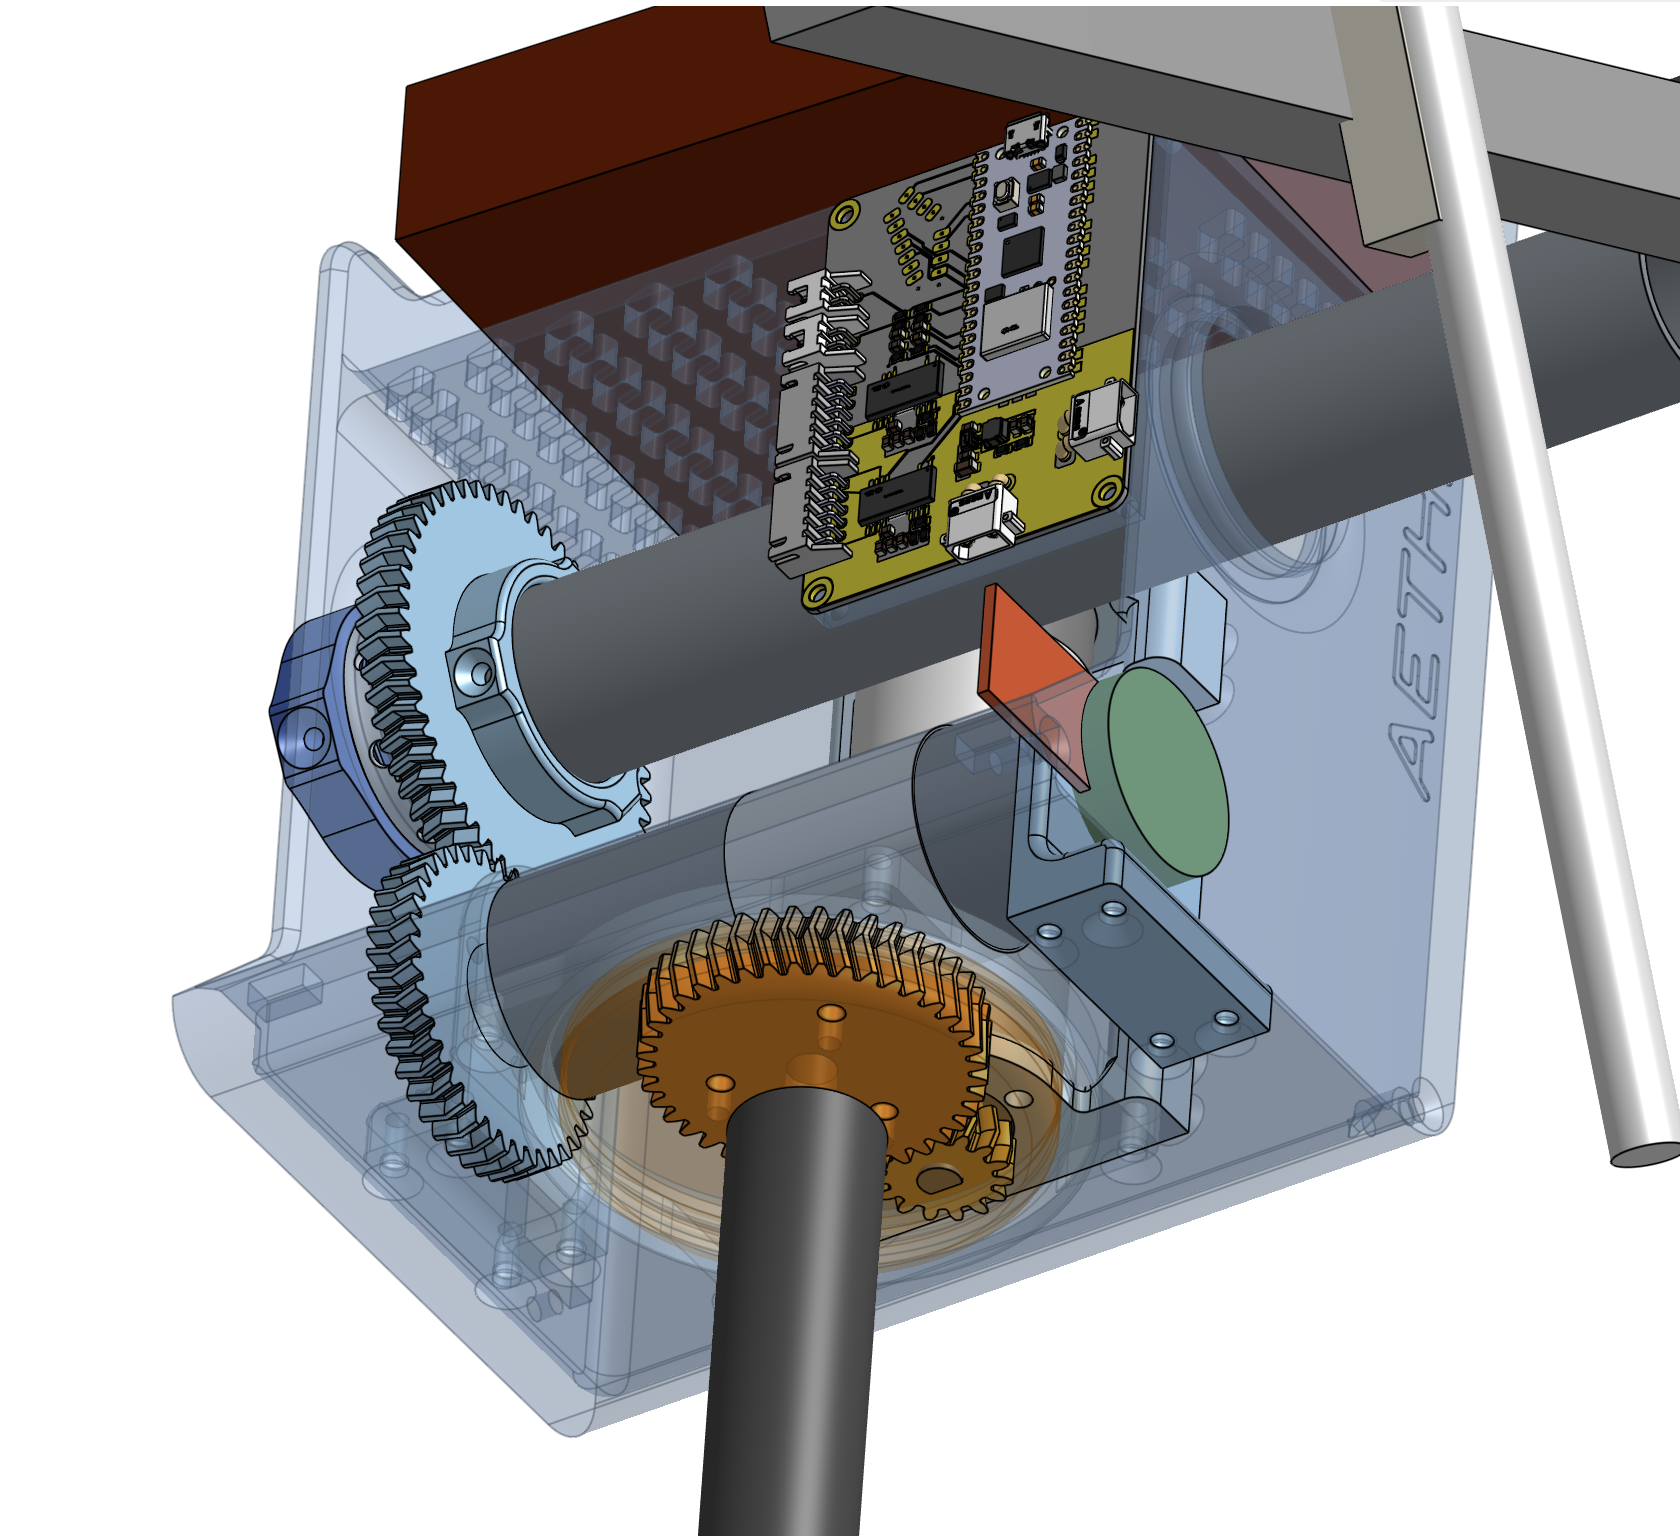
\includegraphics[width=0.7\textwidth]{photos/gears_cad.png}
    \caption{Parametric CAD source of the gear profile, generated in Onshape.}
\end{figure}

\section{Motors}
\label{sec:motors}

The axis motor is the FAPG36-555-EN (FONEACC): a 24~V brushed DC motor with a 516:1 internal planetary gearbox~\cite{fapg36-555}. Manufacturer spec: approximately 16~RPM no-load at 24~V, nominal output torque 4~Nm, 6~mm D-shaft output. A Hall-effect quadrature encoder is mounted on the motor shaft (before the gearbox). The manufacturer datasheet specifies 12~PPR (48~CPR in 4$\times$ decode); the purchased units empirically measure as 16~PPR (64~CPR in 4$\times$ decode), verified by matching firmware encoder counts against known commanded axis rotations during bring-up. The 6~mm D-shaft press-fits directly into the printed gear.

\subsection{Torque budget}

Hanssens~\cite{hanssens2023} identified insufficient stepper torque as the failure mode of his azimuth rotation tests. The DC-motor path chosen here multiplies the manufacturer output torque by the external gear ratio:

\begin{itemize}
    \item AZ: $4~\text{Nm} \times 2.667 = 10.7$~Nm at the output shaft (manufacturer spec $\times$ external ratio).
    \item EL: $4~\text{Nm} \times 1.375 = 5.5$~Nm at the output shaft.
\end{itemize}

\paragraph{Measured output torque.} The assembled rotator was bench-measured with a lever-arm-plus-kitchen-scale setup. A rigid arm attached to the axis output pushes down on the scale at a known radius while the axis is commanded to rotate at 95\,\% duty; the peak scale reading gives the output force.

\begin{itemize}
    \item AZ: 0.71~kgf at 0.50~m lever $\Rightarrow T_\text{AZ} = 0.71 \cdot 9.81 \cdot 0.50 = 3.48$~Nm (Fig.~\ref{fig:torque-az}).
    \item EL: 1.10~kgf at 0.40~m lever $\Rightarrow T_\text{EL} = 1.10 \cdot 9.81 \cdot 0.40 = 4.32$~Nm (Fig.~\ref{fig:torque-el}).
\end{itemize}

Measured EL reaches approximately 80\,\% of the spec-derived 5.5~Nm. Measured AZ reaches approximately 33\,\% of the spec-derived 10.7~Nm; the AZ rig lets the rotor continue to move as the scale deflects, so the reading is the rotating-under-load torque rather than the stalled peak. Both measured values exceed what the Siretta Oscar 44 Yagi (mass $\sim$0.6~kg) requires at the lever of the assembled antenna.

\begin{figure}[H]
    \centering
    \begin{minipage}{0.48\textwidth}
        \centering
        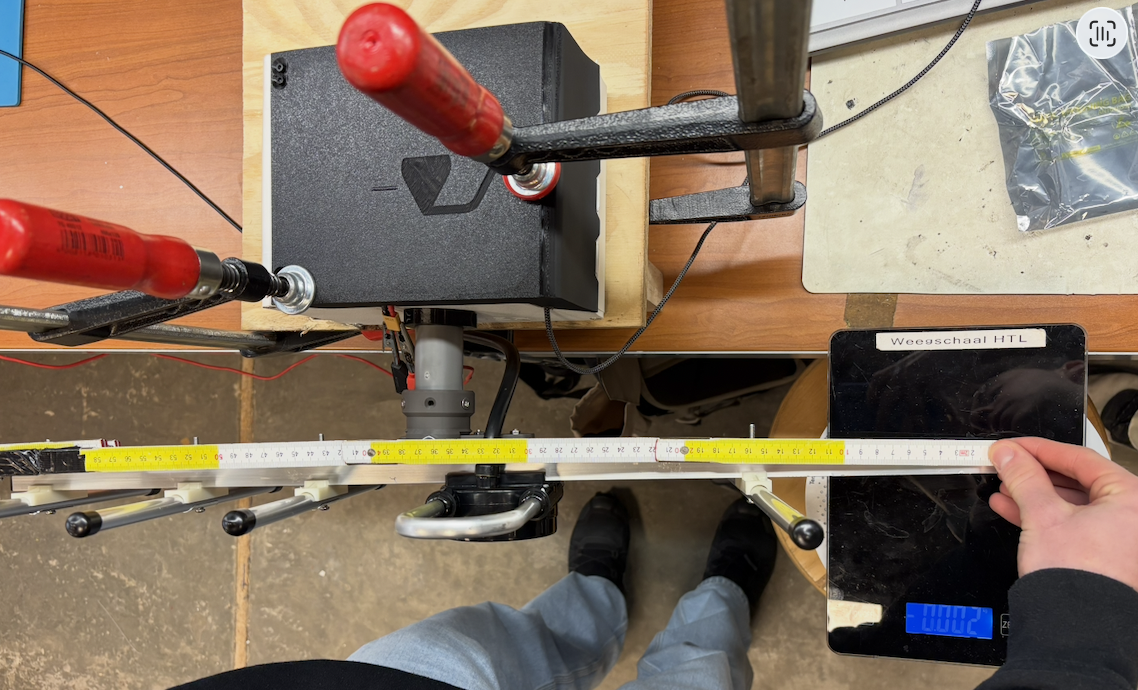
\includegraphics[width=\textwidth]{photos/torque_az_arm.png}
    \end{minipage}\hfill
    \begin{minipage}{0.48\textwidth}
        \centering
        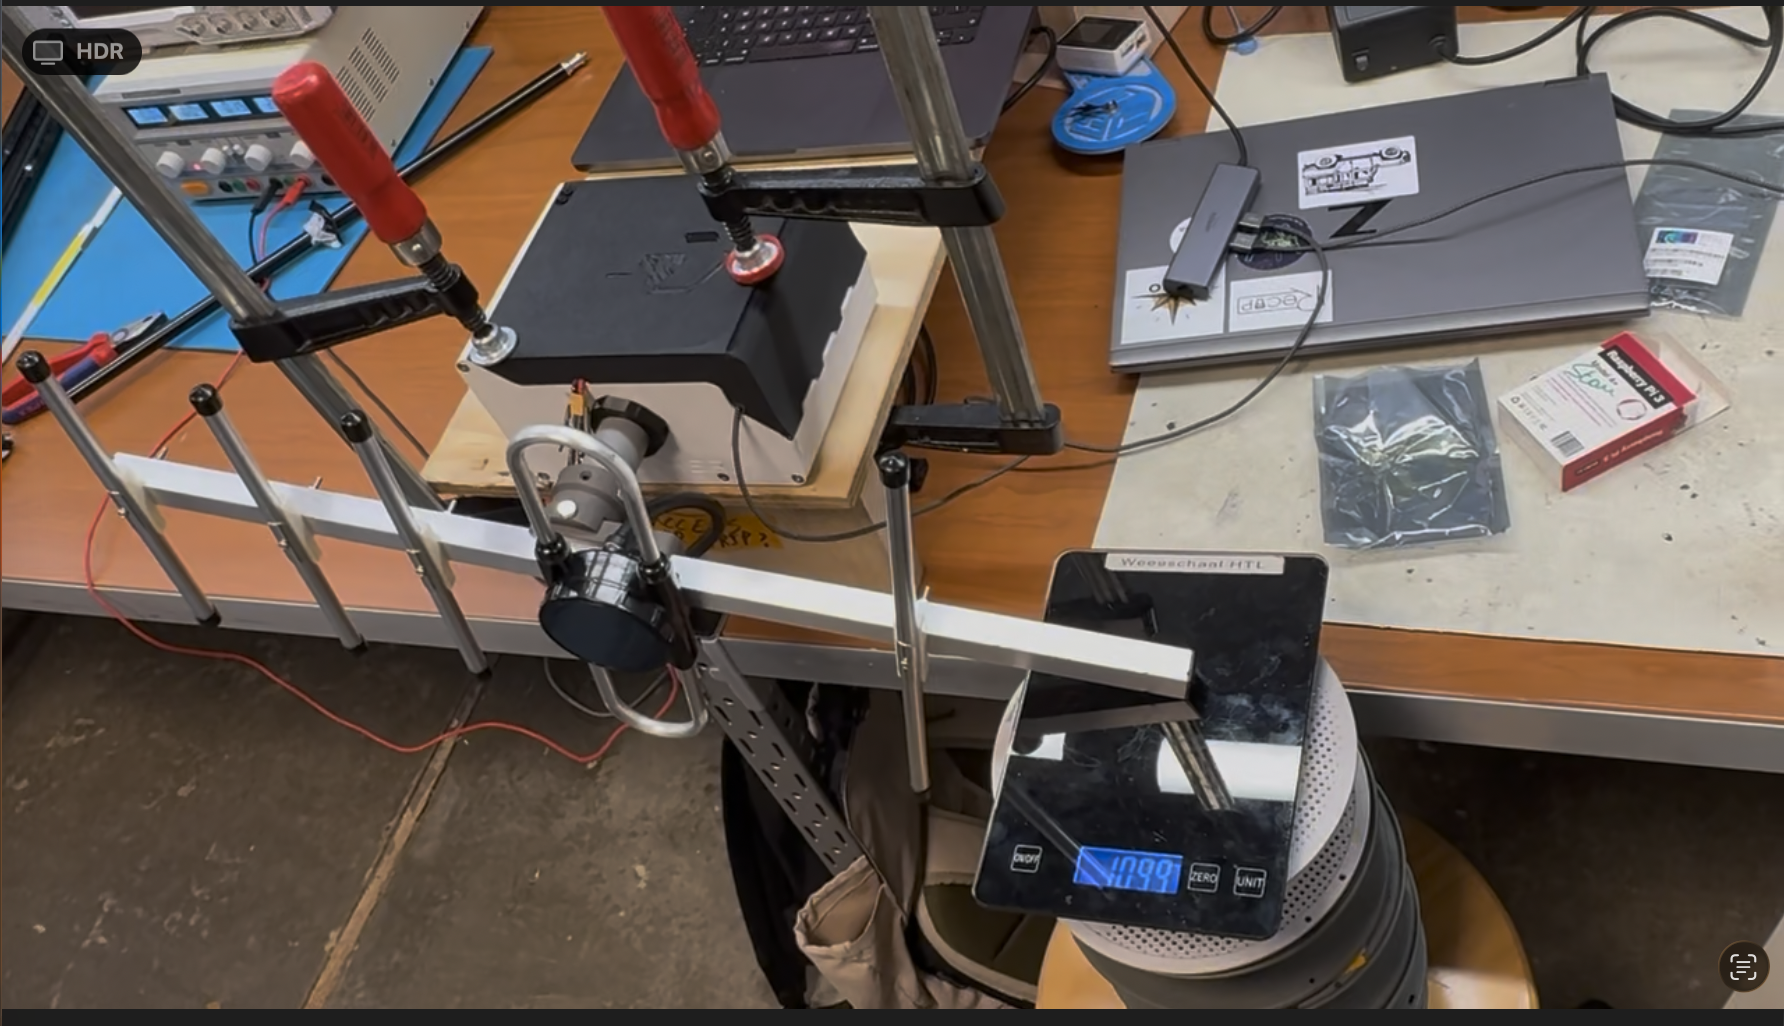
\includegraphics[width=\textwidth]{photos/torque_az_scale.png}
    \end{minipage}
    \caption{AZ torque measurement: 0.50~m lever, scale reads 0.71~kgf $\Rightarrow$ 3.48~Nm.}
    \label{fig:torque-az}
\end{figure}

\begin{figure}[H]
    \centering
    \begin{minipage}{0.48\textwidth}
        \centering
        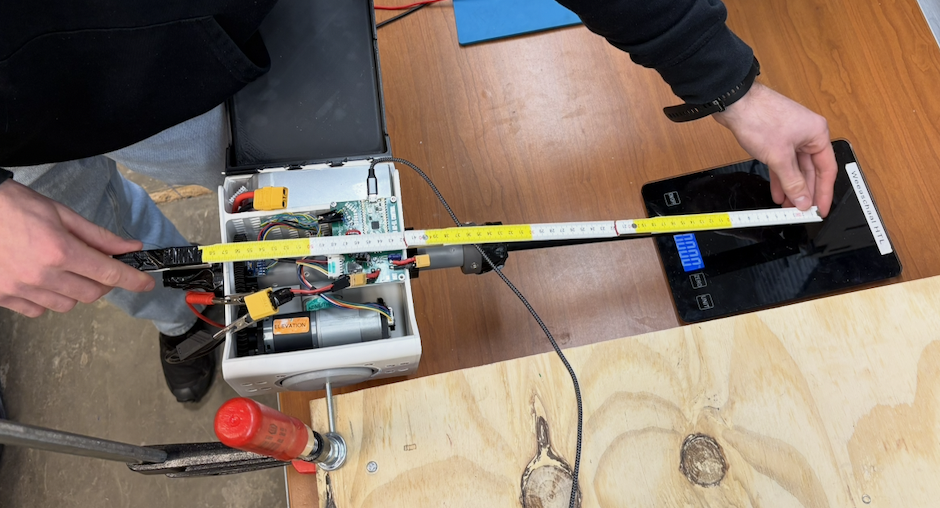
\includegraphics[width=\textwidth]{photos/torque_el_arm.png}
    \end{minipage}\hfill
    \begin{minipage}{0.48\textwidth}
        \centering
        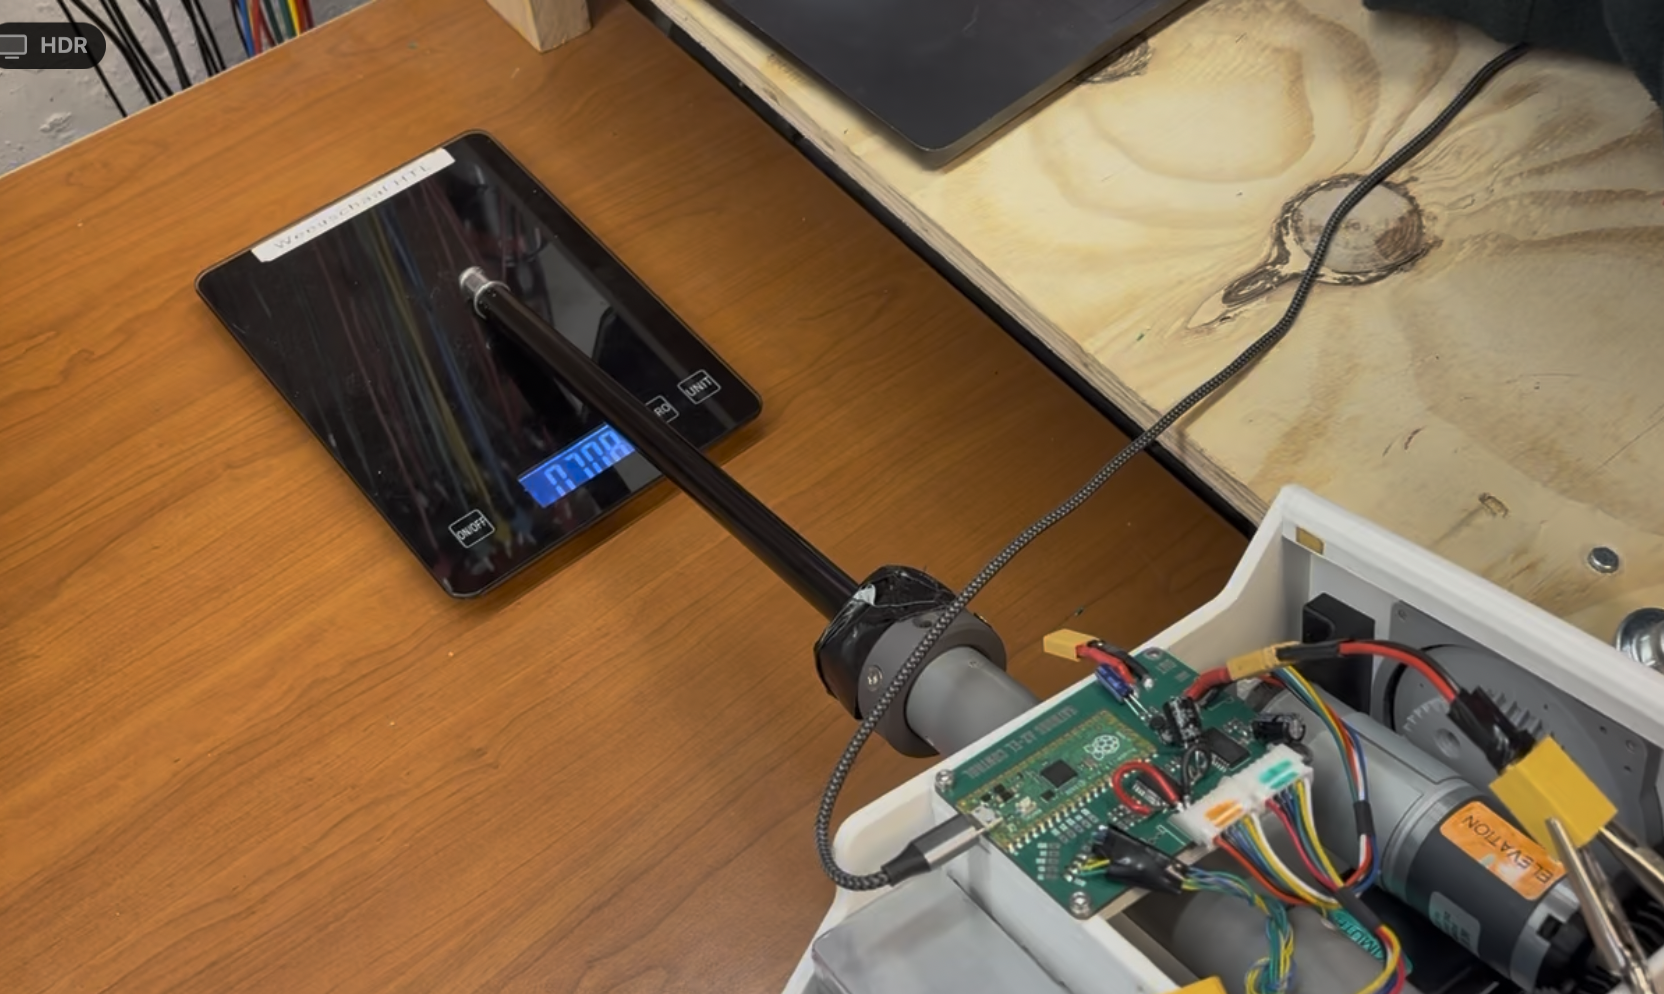
\includegraphics[width=\textwidth]{photos/torque_el_scale.png}
    \end{minipage}
    \caption{EL torque measurement: 0.40~m lever, scale reads 1.10~kgf $\Rightarrow$ 4.32~Nm.}
    \label{fig:torque-el}
\end{figure}

\subsection{DC vs stepper}

The choice of DC motors over stepper motors was informed by Hanssens' torque test~\cite{hanssens2023} and by three properties of the DC-motor-plus-high-ratio-gearbox path:

\begin{enumerate}
    \item Zero idle current with mechanical position holding. A brushed DC motor draws no current when stationary, and a 516:1 reduction makes back-driving from the output side require $516\times$ the static friction torque of the unloaded motor rotor, which for a planetary gearbox of this ratio practically prevents back-drive under wind gusts. The station is unpowered at the motor terminals for the $\sim$90\,\% of the orbit it is idle (about 80 minutes out of a 92-minute orbit, per \S\ref{sec:orbital-mechanics}). In contrast, a stepper requires continuous holding current (typically 0.8--1.5~A per phase at rated current per the Pololu stepper catalogue~\cite{pololu-stepper}) to resist back-drive; a de-energised stepper has no holding torque.
    \item Torque retained at low speed. The 516:1 internal gearbox plus the external stage delivers the torque budget listed above across the full output-speed range used for tracking (0--35\degree/s). Steppers lose torque above their pull-out speed and require microstepping to produce smooth motion, which further reduces available torque per step.
    \item Closed-loop position verification. The quadrature encoder on the motor shaft gives continuous position feedback. A stepper skipping a step (wind gust, obstruction, or torque-curve excursion) silently diverges commanded from actual position unless an external encoder is added; with the encoder already in place here, the PID loop sees any discrepancy within one control period.
\end{enumerate}

The trade-off is firmware complexity: the DC-motor path requires a PID loop and quadrature-decode ISRs (\S\ref{sec:rotator-pid}, \S\ref{sec:quadrature}). The encoder feedback also makes safety features possible (runaway detection, soft-limit enforcement) that a stepper-without-encoder cannot implement.

No slip ring is fitted on the azimuth axis. The firmware tracks cumulative rotation and enforces soft limits at $\pm$360\degree, so the antenna cable never wraps more than one full turn. Between passes, the \code{PARK} command returns the antenna to true-north / zero position via the shortest path, which unwraps any accumulated wrap before the next observation (\S\ref{sec:easycomm}).

\section{Motor Controller PCB}

The v1 MotorPCB is a 4-layer KiCad~9 design with 13 hierarchical sub-sheets, JLCPCB assembled from LCSC basic parts.

Components:
\begin{itemize}
    \item RP2040 (Pi Pico module): EasyComm firmware, PID, encoder ISRs.
    \item 2$\times$ TB6642FG~\cite{tb6642fg}: 50~V absolute-max / 4.5~A peak H-bridge. IN1/IN2 + PWM. 20~kHz PWM frequency.
    \item ADXL345~\cite{adxl345}: 3-axis accelerometer on SPI0, gravity vector for EL homing.
    \item Encoder inputs: 4 GPIO with IRQ, 4$\times$ quadrature decoding. RC filter caps removed (see \S\ref{sec:bringup}).
    \item NeoPixel: optional WS2812B status output: idle = green, tracking = blue, on-target = cyan, fault = red.
\end{itemize}

The fielded v1 firmware uses GP16 for AZ IN1 after the GP15 damage described in \S\ref{sec:bringup}; the schematic's original GP15 assignment is retained only as bring-up history.

\begin{table}[H]
    \centering
    \begin{tabular}{lll}
        \toprule
        Function & AZ pins & EL pins \\
        \midrule
        Motor IN1/IN2/PWM & GP16/GP14/GP22 & GP28/GP27/GP21 \\
        Encoder A/B       & GP11/GP10      & GP12/GP13 \\
        \bottomrule
    \end{tabular}
    \caption{Rotator PCB pin assignments (as-deployed v1).}
\end{table}

\begin{figure}[H]
    \centering
    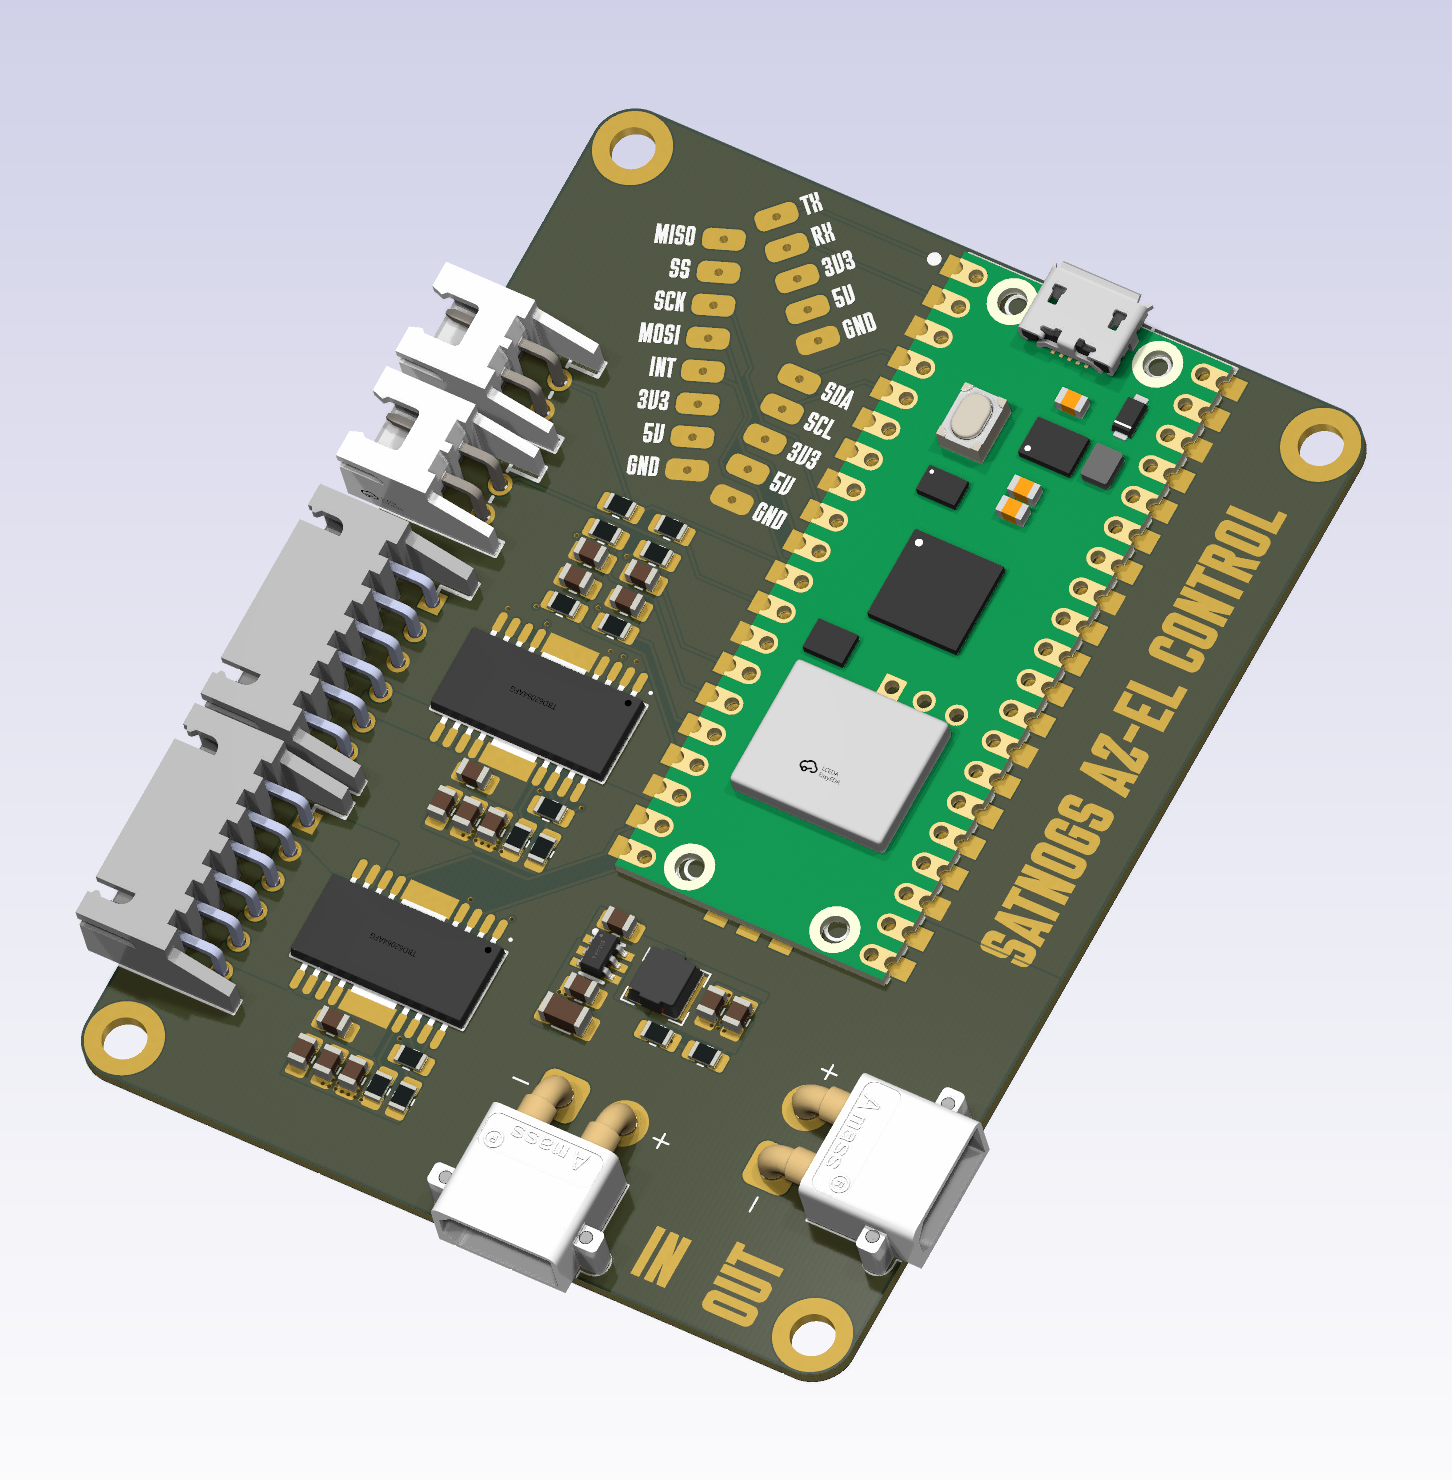
\includegraphics[width=0.7\textwidth]{photos/AZEL_control_front.png}
    \caption{KiCad 3D render of the v1 MotorPCB.}
\end{figure}

\begin{figure}[H]
    \centering
    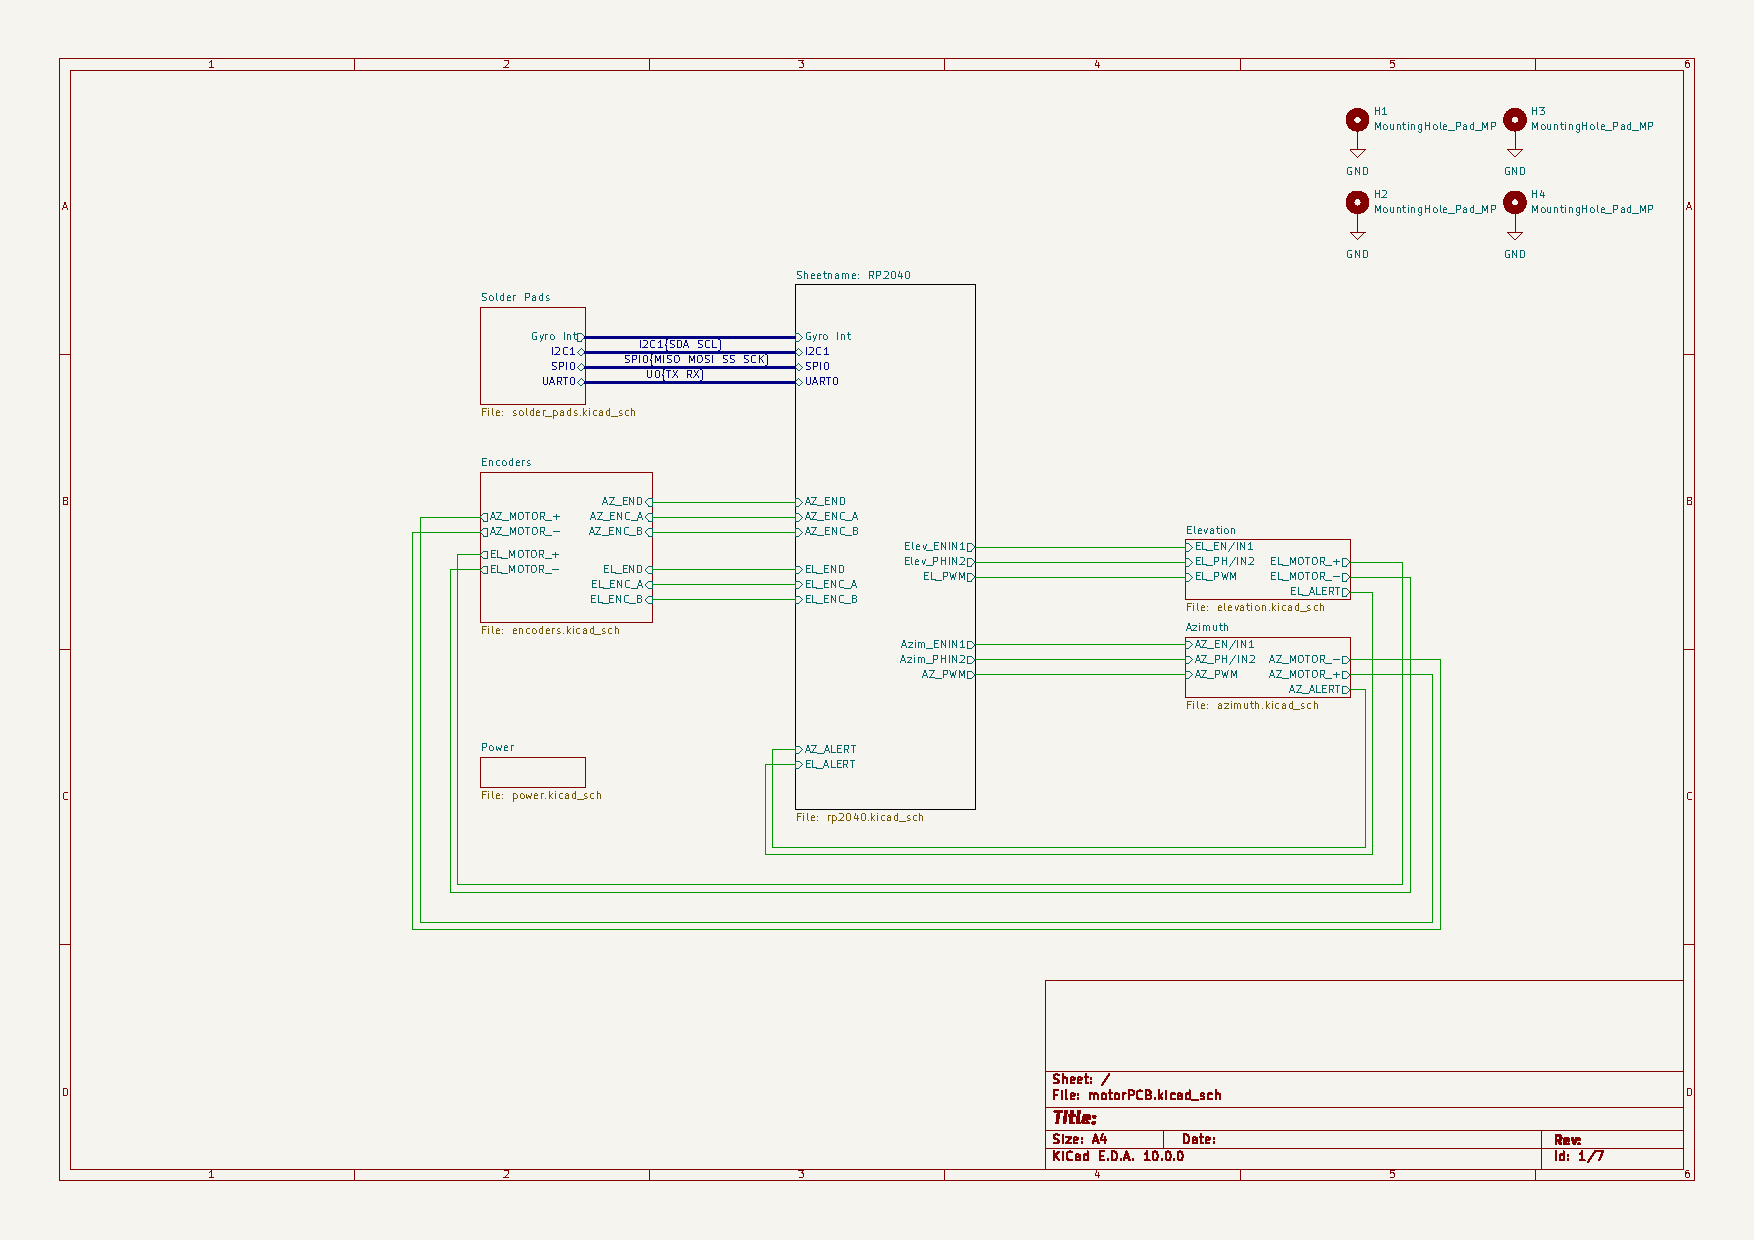
\includegraphics[page=1,width=\textwidth]{schematics/MotorPCB_schematic.pdf}
    \caption{Top-level hierarchical schematic of the v1 MotorPCB. The 13 sub-sheets (RP2040 controller, solder-pad breakouts, encoder front-end, AZ/EL H-bridges, IMU, status LED, USB, power, etc.) are exported in full in the project KiCad repository (\file{MotorPCB/}).}
    \label{fig:motorpcb-schematic}
\end{figure}

\section{Bring-Up and Hardware Debugging}
\label{sec:bringup}

The first-revision MotorPCB shipped with three defects, all fixed with bodge wires and reflected in the v2 design:
\begin{itemize}
    \item Missing EL driver traces. OUT1/OUT2 on the elevation TB6642FG were unrouted; bodged through unused NC pins (6, 11).
    \item Encoder RC filters (C1--C4). 100~nF caps on the Hall-sensor lines low-passed the signal into unusability; removed. Debouncing is handled in firmware.
    \item AZ driver blown by bootloader cycling. The 1200-baud bootloader trick with 24~V connected damaged the TB6642FG IN1 ESD diode and the GP15 pad; driver replaced and IN1 rerouted to GP16.
\end{itemize}

The v2 MOTOR\_RF\_HAT corrects all three natively: routed EL outputs, no encoder caps, and 100\,$\Omega$ series resistors (R11--R14) on every GPIO-to-driver line. Merging the motor controller and RF front-end onto one Pi HAT also removes the USB cable and separate 5\,V path.

\section{Cost}
\label{sec:cost}

Two hardware configurations are priced separately. The first is the as-deployed v1 setup that was used for field validation (a separate MotorPCB and RF~HAT, connected to the Pi via USB and UART respectively); v1 existed to validate the architecture and firmware and to let the RF and rotator subsystems be developed in parallel. The second is the v2 combined MOTOR\_RF\_HAT, the thesis's final hardware deliverable: design-complete, routed, BOM finalised, ready to order but not yet fabricated at the time of writing. v2 reaches $\sim$€40 for the combined controller/RF PCB, $\sim$€75 for the rotator hardware excluding the Pi, and $\sim$€100 for the station core, which misses the strict ``under €50 full rotator'' target once motors and mechanics are included but lands at approximately one-eighth of the cheapest commercial unit (€760 Yaesu G-5500~\cite{yaesu-g5500}).

Component prices from the LCSC BOM tool (April 2026), bare PCB from JLCPCB (5-piece order). Full BOM in Appendix~\ref{app:bom} and \file{ThesisPaper/bom\_complete.csv}.

\subsection{v1 (deployed, field-validated)}

\begin{figure}[H]
    \centering
    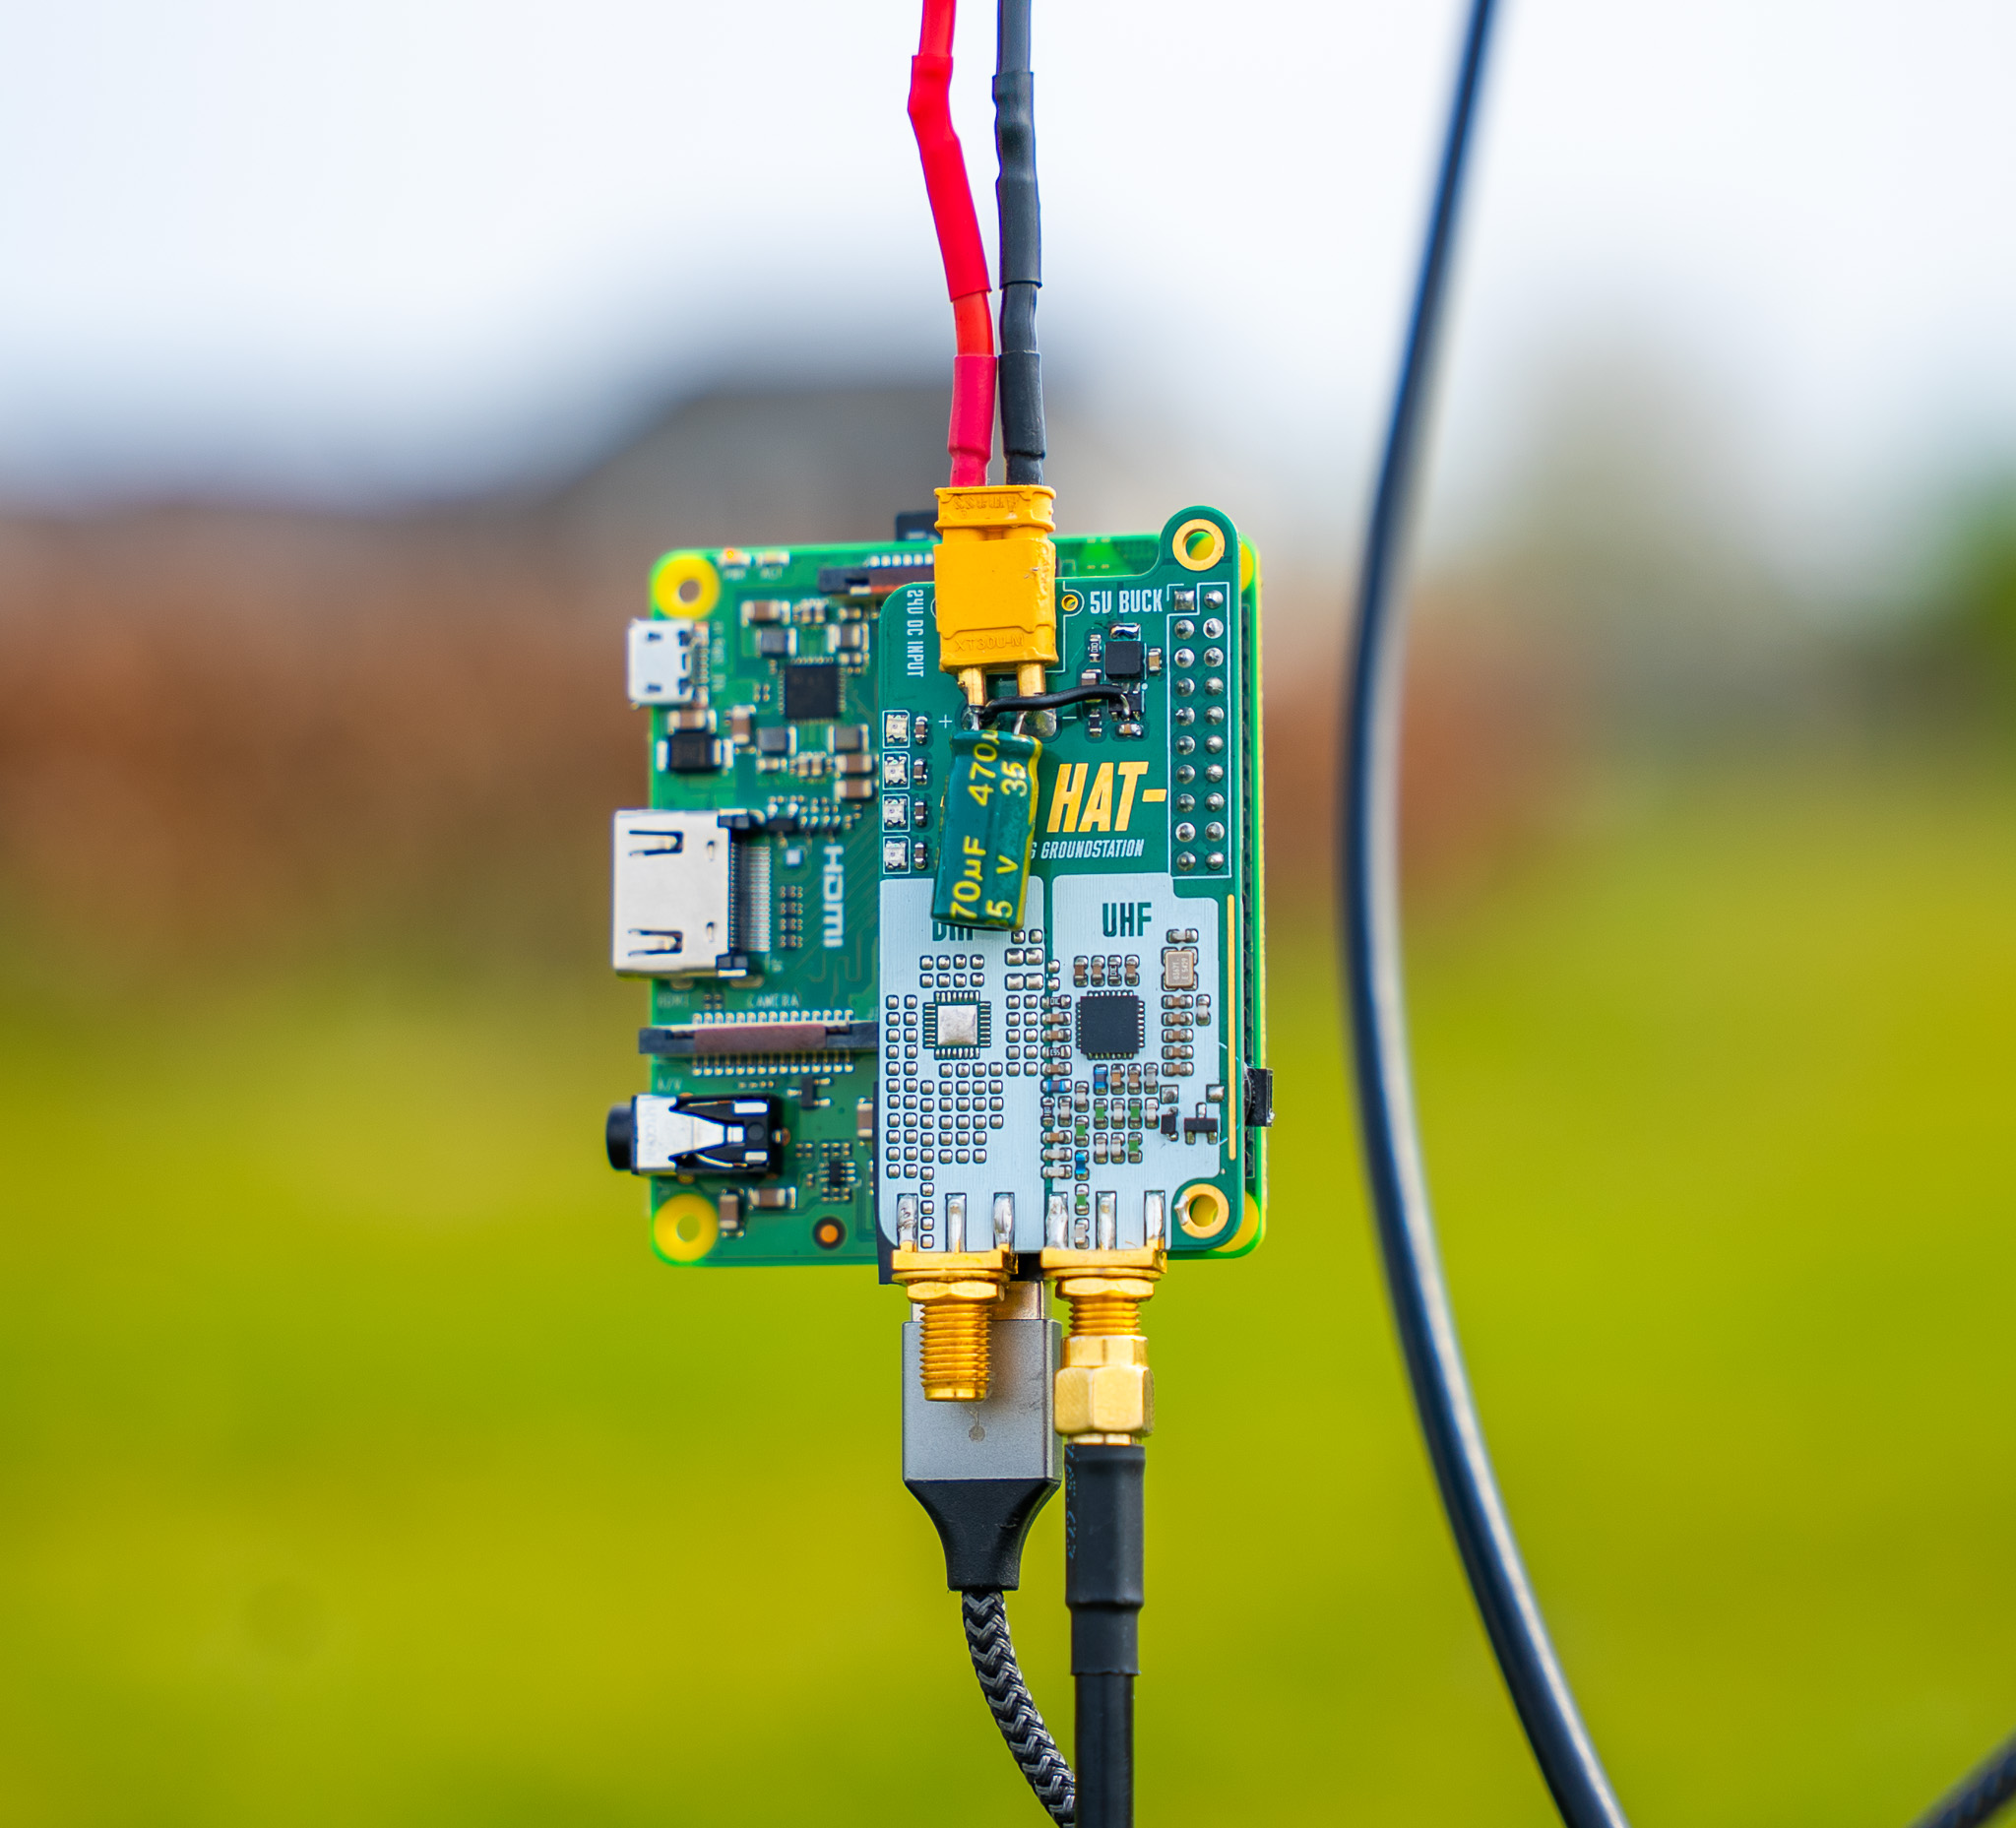
\includegraphics[width=0.7\textwidth]{photos/rf_hat_bench.jpg}
    \caption{v1 RF HAT: 6-layer Pi HAT containing the dual-CC1200 transceivers.}
    \label{fig:rf-hat-front}
\end{figure}

\begin{figure}[H]
    \centering
    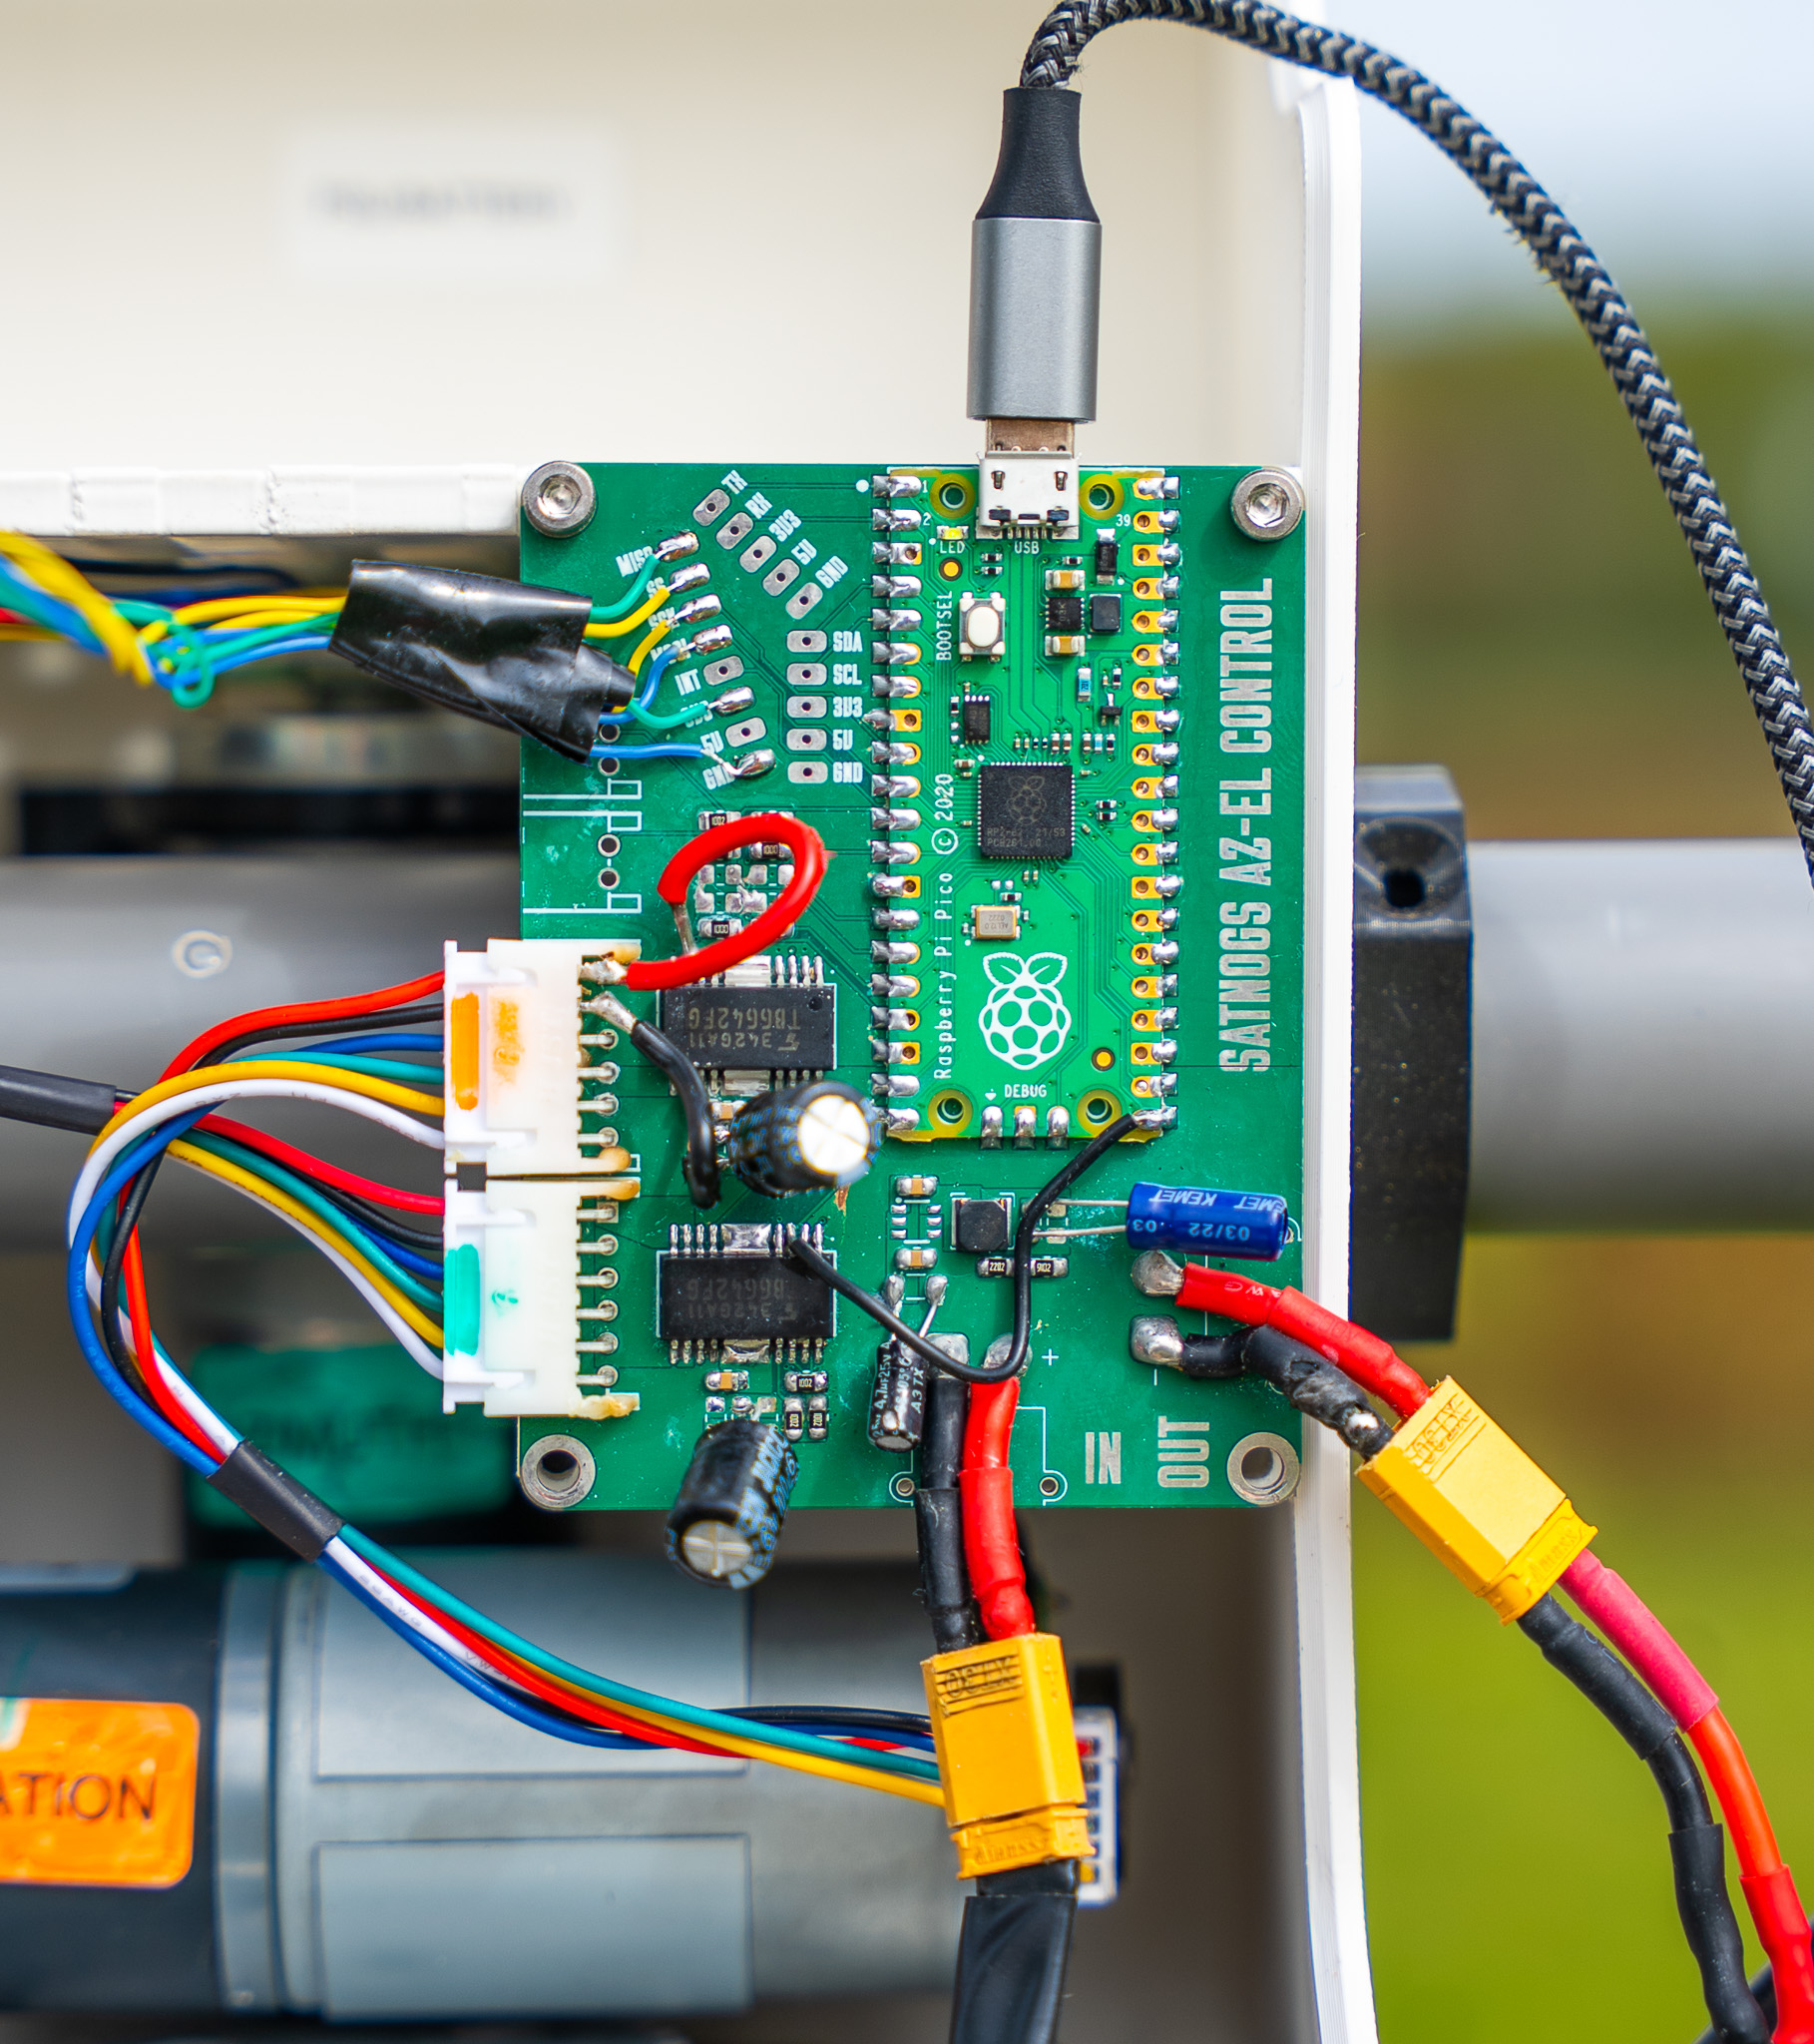
\includegraphics[width=0.7\textwidth]{photos/motorcontrol.jpg}
    \caption{v1 MotorPCB assembled prototype, mounted in the rotator electronics bay.}
\end{figure}

\begin{table}[H]
    \centering
    \begin{tabular}{lr}
        \toprule
        Component & \euro{} \\
        \midrule
        MotorPCB (KiCad 9, 4-layer, 13 sub-sheets, JLCPCB assembled) & $\sim$30 \\
        RF HAT (6-layer Pi HAT, 2$\times$ CC1200, JLCPCB assembled) & $\sim$55 \\
        Raspberry Pi 3 Model A+ & 25 \\
        Mechanical (motors, ASA, bearings, hardware) & $\sim$35 \\
        \midrule
        \textbf{v1 total} & \textbf{$\sim$€145} \\
        \bottomrule
    \end{tabular}
    \caption{v1 (as-deployed) cost breakdown.}
\end{table}

\subsection{v2 (MOTOR\_RF\_HAT, design-complete, ready to order)}

The v2 board merges motor control and RF front-end onto a single 6-layer Pi HAT. The A4950 (SOIC-8-EP) replaces the TB6642FG (HSOP-16) for availability (the TB6642FG went out of stock at JLCPCB during the project), and four 100\,$\Omega$ series resistors (R11--R14) on the GPIO-to-driver lines limit transients during bootloader cycling. One RP2040 handles both motor control and RF, so the USB cable and separate 5~V path are removed. Hand assembly avoids JLCPCB's extended-part setup fee ($\sim$€18/board for the many precise RF L/C values).

\begin{figure}[H]
    \centering
    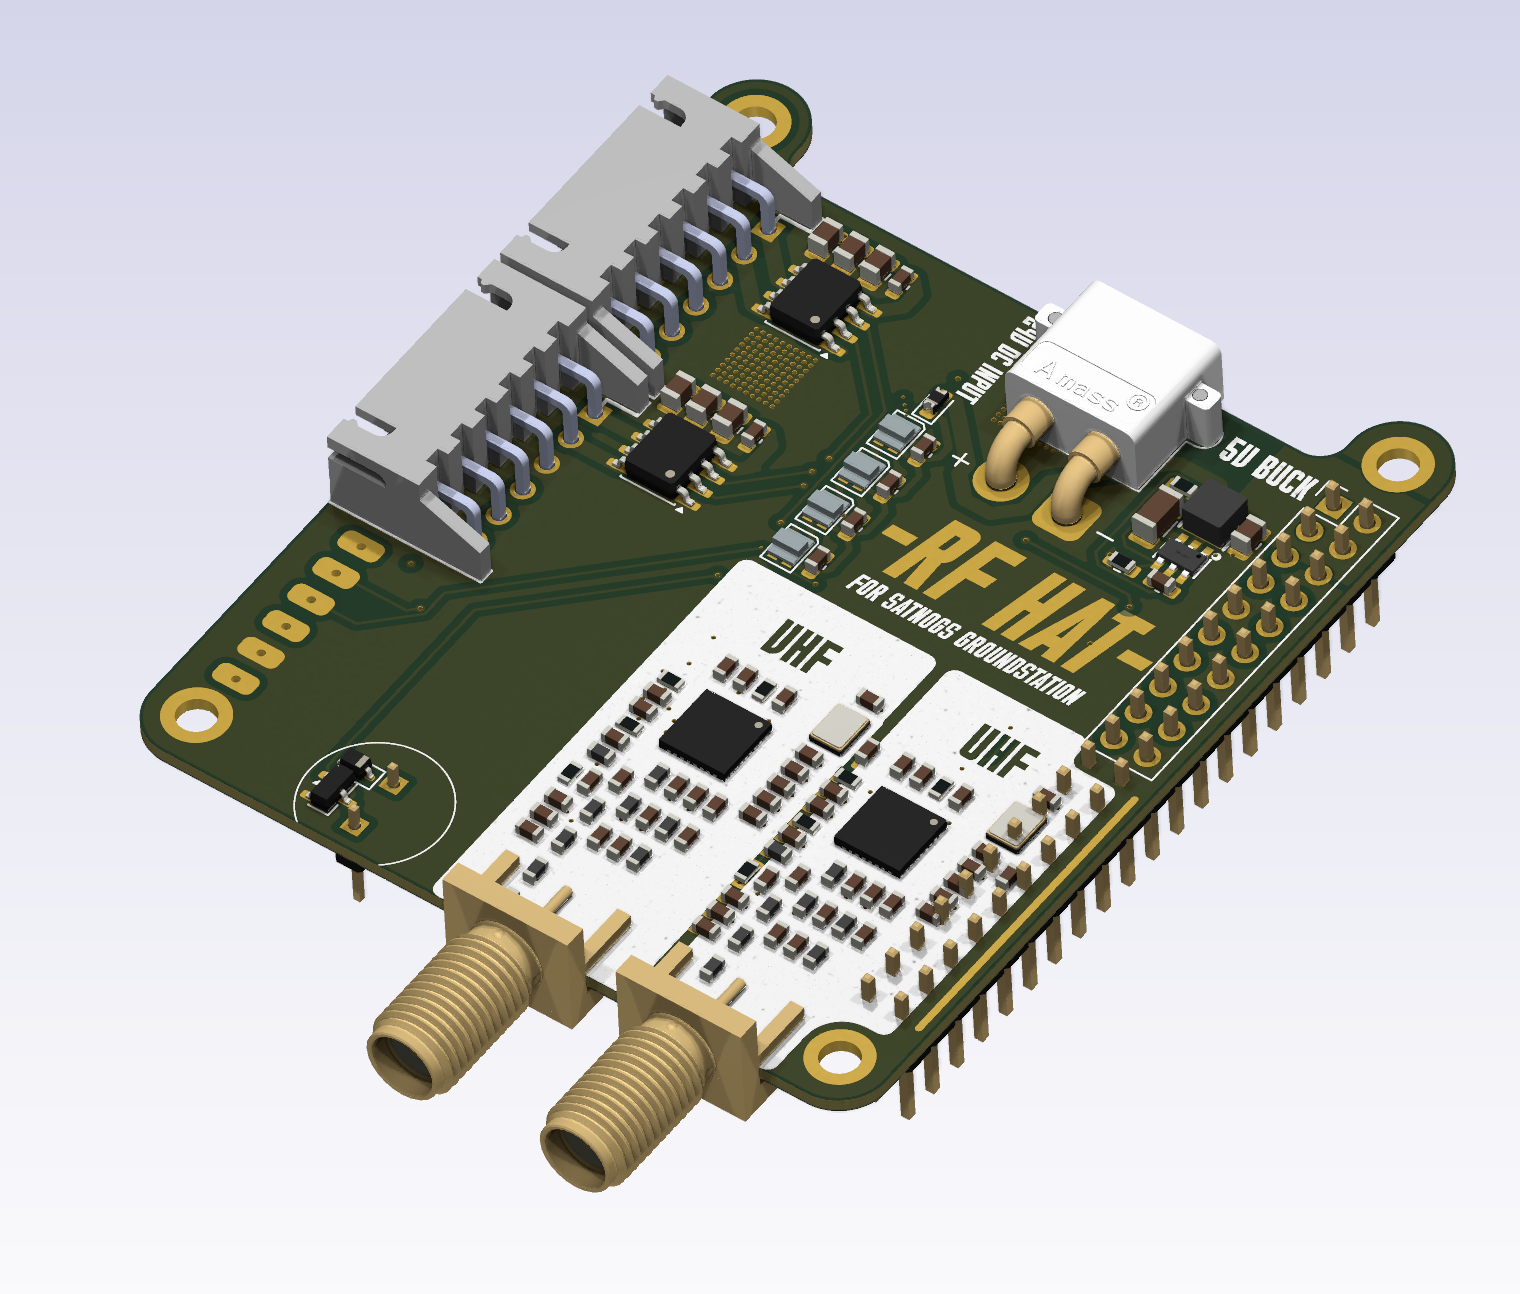
\includegraphics[width=0.7\textwidth]{photos/rf_hat_motor_front.png}
    \caption{v2 MOTOR\_RF\_HAT (front): 6-layer Pi HAT merging motor control and dual-CC1200 RF.}
    \label{fig:motor-rf-hat-front}
\end{figure}

\begin{figure}[H]
    \centering
    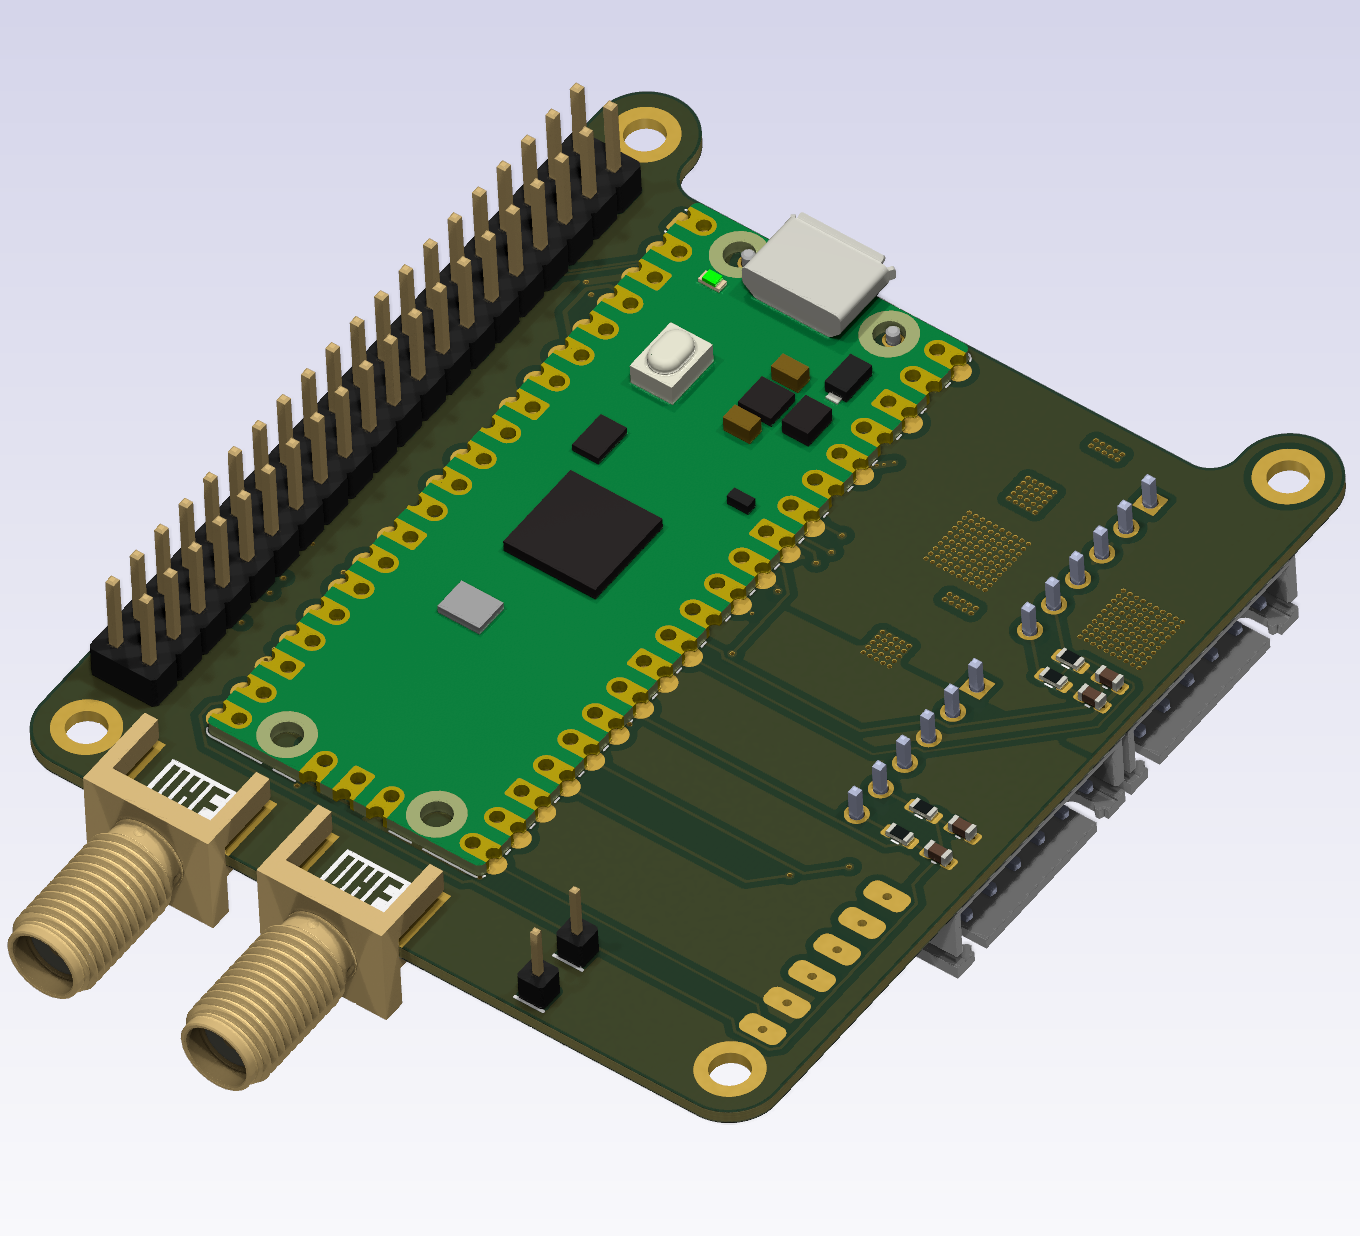
\includegraphics[width=0.7\textwidth]{photos/rf_hat_motor_back.png}
    \caption{v2 MOTOR\_RF\_HAT (back).}
\end{figure}

\begin{table}[H]
    \centering
    \begin{tabular}{lr}
        \toprule
        Component & \euro{} \\
        \midrule
        \multicolumn{2}{l}{\textbf{MOTOR\_RF\_HAT PCB}} \\
        Components (LCSC, incl. MOQ rounding) & 28.44 \\
        SMA connectors + 15~nH inductors (not on LCSC) & 2.00 \\
        Raspberry Pi Pico (hand-soldered) & 4.00 \\
        Bare PCB (6-layer, JLCPCB, per board from 5-pc order) & 6.00 \\
        \textbf{PCB subtotal} & \textbf{$\sim$40} \\
        \midrule
        \multicolumn{2}{l}{\textbf{Off-board}} \\
        FAPG36-555-EN motors (2$\times$) & 16.00 \\
        ASA filament ($\sim$400~g) & 10.00 \\
        Steel balls, screws, heat-set inserts & 5.00 \\
        PVC pipe + misc hardware & 2.00 \\
        ADXL345 IMU breakout & 1.50 \\
        \textbf{Mechanical subtotal} & \textbf{$\sim$35} \\
        \midrule
        \multicolumn{2}{l}{\textbf{Station computer}} \\
        Raspberry Pi 3 Model A+ & 25.00 \\
        \midrule
        \textbf{v2 station-core total} & \textbf{$\sim$€100} \\
        \bottomrule
    \end{tabular}
    \caption{v2 (MOTOR\_RF\_HAT, projected) cost breakdown. Excludes antenna, coax, power supply, and tripod.}
\end{table}

Excludes antenna, coax, power supply, and tripod (user-supplied). v2 brings the rotator BOM (PCB + motors + mechanics, excluding the Pi) to $\sim$€75, or $\sim$€40 for the combined controller/RF PCB alone. This misses a strict full-rotator €50 target but stays well below existing open-source and commercial rotators (Table~\ref{tab:rotator-comparison}).

% ══════════════════════════════════════════════════════════════════════════════
\chapter{RF Front-End}
\label{ch:rf-frontend}
% ══════════════════════════════════════════════════════════════════════════════

\section{RF PCB Design}

The RF PCB implements the front-end architecture responsible for signal transmission, reception, and communication with the host system. This section describes the electrical design of the PCB, including system architecture, component selection, and interconnections between subsystems.

\subsection{System Overview}

The RF PCB is based on a microcontroller-controlled dual-transceiver architecture supporting both the VHF (144\,MHz) and UHF (433\,MHz) frequency bands.

The design consists of the following functional blocks:

\begin{itemize}
\item An RP2040-based microcontroller for system control and data handling
\item Two RF transceivers (VHF and UHF)
\item Dedicated SPI communication interfaces
\item A UART interface to the Raspberry Pi host
\item Power distribution
\end{itemize}

Figure~\ref{fig:motor-rf-hat-front} (Chapter~\ref{ch:system-design}) shows the assembled v2 Pi HAT, which merges this RF architecture with the motor-controller front-end.

\subsection{Microcontroller Subsystem}

The RF PCB is controlled by a Raspberry Pi Pico microcontroller based on the RP2040 \cite{rp2040ds}. This device acts as the central control unit of the RF system.

Its responsibilities include:

\begin{itemize}
\item Configuration of both RF transceivers using SPI
\item Handling of transmit and receive data
\item Communication with the host system via UART
\item Control of auxiliary signals such as chip select and interrupt lines
\end{itemize}

The RP2040 was selected due to its dual-core architecture and availability of two independent hardware SPI peripherals, enabling independent communication with both RF transceivers without bus arbitration \cite{rp2040ds}. Compared to typical single-SPI microcontrollers, this reduces firmware complexity and improves timing determinism.

Furthermore, the platform supports rapid firmware development and iteration through a well-established software ecosystem, enabling efficient testing and debugging during the development process.

\begin{table}[H]
\centering
\caption{RP2040 Pin Assignment for RF PCB}
\begin{tabular}{|c|c|c|}
\hline
\textbf{GPIO} & \textbf{Function} & \textbf{Connected To} \\
\hline
GPIO0  & UART TX & Raspberry Pi RX (J3) \\
GPIO1  & UART RX & Raspberry Pi TX (J3) \\
\hline
GPIO10 & SPI (UHF) SCLK & CC1200 UHF SCLK \\
GPIO11 & SPI (UHF) MOSI & CC1200 UHF SI \\
GPIO12 & SPI (UHF) MISO & CC1200 UHF SO \\
GPIO13 & SPI (UHF) CS   & CC1200 UHF \texttt{\textasciitilde CS} \\
GPIO8  & UHF reset      & CC1200 UHF \texttt{\textasciitilde RESET} \\
GPIO7  & UHF GPIO0      & CC1200 UHF GPIO0 \\
GPIO9  & UHF GPIO2      & CC1200 UHF GPIO2 \\
GPIO6  & UHF GPIO3      & CC1200 UHF GPIO3 \\
\hline
GPIO18 & SPI (VHF) SCLK & CC1200 VHF SCLK \\
GPIO19 & SPI (VHF) MOSI & CC1200 VHF SI \\
GPIO16 & SPI (VHF) MISO & CC1200 VHF SO \\
GPIO17 & SPI (VHF) CS   & CC1200 VHF \texttt{\textasciitilde CS} \\
GPIO20 & VHF reset      & CC1200 VHF \texttt{\textasciitilde RESET} \\
GPIO22 & VHF GPIO0      & CC1200 VHF GPIO0 \\
GPIO21 & VHF GPIO2      & CC1200 VHF GPIO2 \\
GPIO26 & VHF GPIO3      & CC1200 VHF GPIO3 \\
\hline
\end{tabular}
\end{table}

\subsection{RF Transceiver Subsystem}

The RF PCB employs two CC1200 transceivers to enable dual-band operation \cite{cc1200}. Each transceiver can operate independently and includes its own supporting circuitry:

\begin{itemize}
\item A 40\,MHz crystal oscillator
\item External matching and filtering electronics
\item Decoupling capacitors for supply stabilization
\end{itemize}

The use of two dedicated transceivers eliminates the need for an external band-select relay between UHF and VHF, simplifying the signal path and avoiding additional insertion losses.

Key control and interface signals include SPI communication lines, interrupt outputs (the CC1200 GPIO pins), and device control signals such as reset.

The detailed layout and matching-network design of the RF front-end are discussed in the following sections.

\subsection{Communication Interfaces}

\subsubsection{SPI Communication}

Each RF transceiver is connected to the microcontroller via a dedicated hardware SPI interface on the RP2040.

The SPI interfaces consist of the following signals:

\begin{itemize}
\item Serial clock (SCLK)
\item Master-out slave-in (MOSI)
\item Master-in slave-out (MISO)
\item Chip select (CS)
\end{itemize}

Interrupt lines from each transceiver are connected to the microcontroller to signal events such as packet reception or transmission completion.

Using separate SPI buses avoids contention and ensures deterministic communication timing.

\subsubsection{UART Interface to Host}

Communication between the RF PCB and the Raspberry Pi host is implemented via a UART interface.

This interface is used for:

\begin{itemize}
\item Transferring received RF data to the host
\item Receiving configuration and control commands
\item Debugging and diagnostic output
\end{itemize}

\subsection{Power Distribution Network}

The RF PCB is powered from a 24\,V supply via an XT30 connector. This input voltage is converted to a regulated 5\,V rail using an LMR51420 buck converter \cite{lmr51420}. The resulting 5\,V supply is used both to power the Raspberry Pi host through the board header and to supply the VSYS input of the Raspberry Pi Pico microcontroller.

Using a single 5\,V rail for both the host and the onboard controller simplifies the overall power architecture and reduces the required component count.

The Raspberry Pi Pico generates the required 3.3\,V rail using its onboard RT6150 switching regulator \cite{rt6150}. This 3.3\,V supply powers both CC1200 transceivers as well as the associated digital circuitry on the RF PCB. While switching regulators typically introduce more noise compared to dedicated low-noise linear regulators, the integrated solution provides adequate current capability and efficiency for the system.

Given the noise sensitivity of RF circuits, particular attention was paid to supply integrity. Local decoupling capacitors were placed close to the supply pins of each active component to reduce high-frequency noise, provide transient current during switching events, and improve overall system stability. In addition, careful PCB layout practices were applied to minimize coupling of digital switching noise into the RF signal paths.

\subsubsection{Power Supply Noise Evaluation}

Oscilloscope measurements were performed at the 3.3\,V pins of the CC1200 transceivers to assess voltage stability and switching noise characteristics. The measurements were conducted under multiple operating conditions, including idle, receive, and transmit modes.

The observed DC supply voltage was approximately \textbf{[X.XX\,V]}. The measured peak-to-peak ripple on the 3.3\,V rail was approximately \textbf{[XX\,mV\textsubscript{pp}]} under nominal operation, with transient deviations up to \textbf{[XX\,mV]} observed during mode transitions.

No significant voltage drops or disturbances were observed that could affect the stability of the RF transceivers. Furthermore, the system demonstrated reliable communication during operation, indicating that the supply quality was sufficient for the intended application.

These results scope the 3.3\,V supply rail at the CC1200 pins to within the transceiver's supply-ripple requirements. In-band RF noise at the antenna (characterised in \S\ref{sec:packet-reception}) is a separate concern driven by board-level radiated/conducted interference, not by supply-rail quality; the principal mitigation is a mast-mounted LNA (\S\ref{sec:future-work}). For future iterations, a dedicated low-noise LDO on the RF section may be considered to further improve supply integrity.

\subsection{Summary}

The RF PCB electrical design integrates a microcontroller, dual RF transceivers, and dedicated communication interfaces into a modular and robust architecture. This design forms the foundation for the RF layout considerations discussed in the following sections.

% ──────────────────────────────────────────────────────────────────────────────
\section{RF PCB Layout Considerations}

The performance of the RF front-end is strongly influenced by the PCB layout. While both the 144\,MHz (VHF) and 433\,MHz (UHF) bands are sub-GHz and thus relatively low in frequency compared to microwave systems, careful RF design is still required to ensure impedance control, minimize losses, and reduce electromagnetic interference.

On an early bench prototype, a 4-layer stackup was considered sufficient because compact size was not yet a constraint. However, to achieve the compact form factor of a Raspberry Pi HAT, a 6-layer stackup was used for the final design.

\subsection{6-Layer Stackup Strategy}

The PCB is implemented using JLCPCB's \texttt{JLC06121H-3313} 6-layer stackup with a finished thickness of 1.14\,mm \cite{jlcpcb_stackup}.

\begin{table}[H]
    \centering
    \caption{6-layer PCB stackup (\texttt{JLC06121H-3313}) with electrical function and material properties \cite{jlcpcb_stackup}.}
    \small
    \renewcommand{\arraystretch}{1.2}
    \begin{tabularx}{\textwidth}{l l l l c X}
        \toprule
        \textbf{Layer} & \textbf{Type} & \textbf{Thickness} & \textbf{Material} & \textbf{$\varepsilon_r$} & \textbf{Function} \\
        \midrule
        F.Cu   & Copper       & 0.035\,mm (1\,oz)   & -       & -    & RF routing, matching networks, SMA feedlines \\
        Dielectric 1 & Prepreg 3313 & 0.0994\,mm & NP-155F & 4.1  &  \\
        In1.Cu & Copper       & 0.0152\,mm (0.5\,oz)& -       & -    & Primary ground plane (RF return path) \\
        Dielectric 2 & Core   & 0.35\,mm            & NP-155F & 4.36 &  \\
        In2.Cu & Copper       & 0.0152\,mm (0.5\,oz)& -       & -    & Power distribution (3.3\,V, 5\,V) \\
        Dielectric 3 & Prepreg 2116 & 0.1088\,mm & NP-155F & 4.16 &  \\
        In3.Cu & Copper       & 0.0152\,mm (0.5\,oz)& -       & -    & Secondary ground plane (coupling reduction) \\
        Dielectric 4 & Core   & 0.35\,mm            & NP-155F & 4.36 &  \\
        In4.Cu & Copper       & 0.0152\,mm (0.5\,oz)& -       & -    & Digital and control signal routing \\
        Dielectric 5 & Prepreg 3313 & 0.0994\,mm & NP-155F & 4.1  &  \\
        B.Cu   & Copper       & 0.035\,mm (1\,oz)   & -       & -    & Auxiliary signals and component placement \\
        \bottomrule
    \end{tabularx}
\end{table}

This stackup ensures that RF traces on the top layer (F.Cu) are implemented as controlled-impedance microstrip lines referenced to the continuous ground plane on In1.Cu. This keeps the current return path and loop area minimal, and prevents additional radiation and impedance discontinuities.
The use of two ground planes (In1.Cu and In3.Cu) improves electromagnetic shielding and reduces coupling between RF and digital layers. Additionally, separating digital routing on In4.Cu minimizes interference with sensitive RF signals on the top layer.

\subsection{Transmission Line Implementation}

All RF signal paths are routed with controlled impedance considerations, targeting a characteristic impedance of 50\,$\Omega$, which is standard for RF systems and ensures proper matching with external components.

The characteristic impedance of a microstrip line can be approximated using the narrow-strip Hammerstad expression \cite{pozar}:

\begin{equation}
Z_0 = \frac{60}{\sqrt{\varepsilon_{\text{eff}}}}
\ln \left( \frac{8h}{w} + \frac{w}{4h} \right)
\end{equation}

with the effective dielectric constant given by:

\begin{equation}
\varepsilon_{\text{eff}} = \frac{\varepsilon_r + 1}{2}
+ \frac{\varepsilon_r - 1}{2}
\left( \frac{1}{\sqrt{1 + 12h/w}} \right)
\end{equation}

where $w$ is the trace width, $h$ is the dielectric height between the trace and the ground plane, and $\varepsilon_r$ is the relative permittivity of the substrate. This form is strictly valid for $w/h < 1$; for wider traces a modified expression applies, though the two forms converge near the transition point.

Applying these expressions with the selected stackup parameters ($h = 0.0994$\,mm, $\varepsilon_r = 4.1$) yields an initial estimate of $w \approx 0.20$\,mm. This analytical result does not account for copper thickness. Cross-validating with the JLCPCB impedance calculator \cite{jlcpcb_impedance}, which implements a full numerical model including the finite copper thickness (1\,oz, 0.035\,mm), yields $w = 0.1565$\,mm for a 50\,$\Omega$ single-ended non-coplanar microstrip on this stackup. The KiCad net class was set to 0.15\,mm (6\,mil), the nearest standard routing increment, corresponding to approximately 52--53\,$\Omega$, which is within accepted tolerance for the operating frequencies.

At the operating frequencies, the free-space wavelengths are approximately 2.08\,m at 144\,MHz and 0.69\,m at 433\,MHz. Since the physical dimensions of the matching network (approximately 10\,mm $\times$ 15\,mm) remain well below $\lambda/10$, the interconnects are electrically short and distributed effects are limited.

In theory, grounded coplanar waveguide (GCPW) is often preferred for RF routing due to its improved field confinement, reduced radiation, and better isolation from surrounding structures. However, GCPW requires additional lateral spacing and via fencing, which increases the required board area. Due to the compact form-factor constraints of the Raspberry Pi HAT, microstrip routing was selected as a practical alternative.

By maintaining a continuous ground reference, minimizing trace lengths, and applying sufficient ground stitching, the performance degradation is expected to remain limited.

\subsection{Frequency-Dependent Layout Considerations}

Although both frequency bands share the same PCB layout strategy, their sensitivity to layout effects differ.

At 144\,MHz, the wavelength is relatively large, and PCB interconnects behave predominantly as lumped elements. As a result, the layout is relatively tolerant to small discontinuities and parasitic effects.

At 433\,MHz, however, the shorter wavelength makes PCB parasitics more significant. RF traces must therefore be treated as transmission lines, requiring controlled impedance routing, short interconnects, and dense via stitching to maintain a stable ground reference.

To ensure reliable operation across both bands, the PCB layout is designed according to the more stringent requirements of the 433\,MHz band. This guarantees that performance at 144\,MHz is inherently satisfied.

\subsection{Summary}

A 6-layer PCB stackup was selected to enable a compact RF front-end while maintaining controlled impedance routing and effective isolation between RF, power, and digital domains. The layout is designed according to the more stringent requirements of the 433\,MHz band, ensuring reliable operation across both frequency bands within the given form factor constraints.

% ──────────────────────────────────────────────────────────────────────────────
\section{RF Matching Network}

\subsection{CC1200 RF Interface Characteristics}

To properly design the matching network, it is necessary to consider the RF interface characteristics of the CC1200 as specified in the datasheet \cite{cc1200}.

\subsubsection{Operating Frequency Bands}

There are TI designs for operation in the following frequency ranges:

\begin{itemize}
    \item 164--190\,MHz
    \item 410--475\,MHz
    \item 820--960\,MHz
\end{itemize}

These bands correspond to typical ISM and SRD applications. Operation outside these ranges may be possible but requires careful validation. \cite{cc1200}

\subsubsection{CC1200 RF IO Structure}

The receiver input of the CC1200 consists of a differential low-noise amplifier (LNA) with input pins \texttt{LNA\_P} and \texttt{LNA\_N}. These pins require a DC path to ground and are intended to be driven by a differential RF signal \cite{cc1200}.

The transmitter output is single-ended at the \texttt{PA} pin and requires a DC path to the supply voltage.

In addition, the CC1200 provides a \texttt{TRX\_SW} output pin that the chip drives high during transmission and low during reception \cite{cc1200}. The external matching network uses this switching signal to route signals between the PA output, the LNA input, and the shared antenna port. During transmission, \texttt{TRX\_SW} couples the PA output through the TX matching path to the SMA connector; during reception, it decouples the PA and connects the antenna signal through a coupling network to the differential LNA inputs. This mechanism allows a single SMA connector per transceiver to serve both transmit and receive without an external RF switch.

\subsubsection{Optimum Source Impedance (Receiver)}

The CC1200 does not present a fixed 50\,$\Omega$ input impedance. Instead, the optimal source impedance is frequency-dependent and complex. The datasheet provides reference values for the two bands most relevant to this design \cite{cc1200}:

\begin{itemize}
    \item 433\,MHz band:
    \begin{itemize}
        \item Differential: $100 + j60\,\Omega$
        \item Single-ended equivalent: $50 + j30\,\Omega$
    \end{itemize}
    \item 169\,MHz band (closest datasheet entry to the 144\,MHz design target):
    \begin{itemize}
        \item Differential: $140 + j40\,\Omega$
        \item Single-ended equivalent: $70 + j20\,\Omega$
    \end{itemize}
\end{itemize}

No datasheet entry exists for 144\,MHz. The 169\,MHz values are used as the nearest available reference; the 144\,MHz matching network was designed by scaling component values accordingly (see Section~\ref{sec:matching-topology}).

These values represent the optimum impedance for maximum receiver sensitivity and must be realized through the external matching network.

\subsubsection{Optimum Load Impedance (Transmitter)}

Similarly, the transmitter output requires impedance matching to a complex load. The datasheet specifies \cite{cc1200}:

\begin{itemize}
    \item 433\,MHz band: $55 + j25\,\Omega$
    \item 169\,MHz band (closest reference to the 144\,MHz design target): $80 + j0\,\Omega$
\end{itemize}

This further emphasizes that the RF interface is not inherently matched to 50\,$\Omega$, and external matching is mandatory.

\subsubsection{Receiver Sensitivity and Matching Impact}

The CC1200 achieves high sensitivity, for example:

\begin{itemize}
    \item Up to $-123$\,dBm at 1.2\,kbps 2-FSK with 4\,kHz deviation and 11\,kHz channel filter bandwidth in the 433\,MHz band
\end{itemize}

This performance is specified under optimal matching conditions at the antenna port. Any mismatch between the antenna and the IC will degrade sensitivity due to reduced power transfer and increased noise figure. \cite{cc1200}

\subsubsection{Output Power and Power Consumption}

The transmitter is capable of delivering \cite{cc1200}:

\begin{itemize}
    \item Up to +16\,dBm at 433\,MHz with a 3.3\,V supply rail
    \item Programmable output power with 0.4\,dB step size
\end{itemize}

At this output level, the current consumption is approximately:

\begin{itemize}
    \item 46--49\,mA in high-performance mode at 433\,MHz
\end{itemize}

These values highlight the importance of efficient matching to avoid unnecessary power loss.

\subsubsection{Implications for Matching Network Design}

The combination of:
\begin{itemize}
    \item Complex, frequency-dependent RF impedance
    \item Differential receiver input
    \item Single-ended transmitter output
    \item Shared antenna port for TX and RX via \texttt{TRX\_SW}
\end{itemize}

necessitates the use of a multi-element matching network that performs impedance transformation, single-ended to differential conversion, and TX/RX path routing simultaneously.

This justifies the use of the three-path LC topology implemented in this work, rather than a simple L-section network.

\subsection{Matching Network Topology}
\label{sec:matching-topology}

\subsubsection{433\,MHz Front-End (Validated Design)}

The implemented 433\,MHz matching network is realized between SMA connector J1 and CC1200 transceiver U1, based on the TI CC1200EM reference design for the 420--470\,MHz band \cite{swrr122} and the M17 CC1200\_HAT Rev~B hardware \cite{m17cc1200hat}. The network is organized across three functional paths:

\begin{itemize}
    \item \textbf{TX matching path}: series inductors L1 (15\,nH), L2 (43\,nH), and L3 (22\,nH) transform the PA output impedance to 50\,$\Omega$, with feedback capacitor C1 (2.2\,pF), series capacitor C2 (39\,pF), shunt capacitor C4 (6.2\,pF), and DC-blocking capacitor C10 (1\,nF) at the SMA interface.
    \item \textbf{PA supply bias path}: RF choke L4 (56\,nH) and bypass capacitor C5 (56\,pF) provide the required DC supply path to the \texttt{PA} pin while presenting high impedance to RF signals.
    \item \textbf{TRX coupling and LNA balun}: inductor L5 (15\,nH) and capacitor C3 (5.1\,pF) form the \texttt{TRX\_SW}-driven coupling network. The differential LNA input is driven through bridge inductor L7 (56\,nH) connecting \texttt{LNA\_P} and \texttt{LNA\_N}, with bias inductors L6 and L8 (27\,nH each) and coupling/shunt capacitors C8 and C9 (5.1\,pF each).
\end{itemize}

This multi-element structure provides gradual impedance transformation, improved bandwidth stability, and additional harmonic filtering compared to a simple L-section network.

\subsubsection{144\,MHz Front-End (Optional, Not Populated)}

In addition to the validated 433\,MHz front-end, the PCB includes an optional 144\,MHz RF path between SMA connector J2 and transceiver U2. The component values were derived by adapting the topology of the TI CC1120EM 169\,MHz reference design \cite{tidr220} and scaling for operation at 144\,MHz. As no official TI reference design exists for 136--160\,MHz, inductor values were scaled by approximately 17\,\% relative to the 169\,MHz design. The three-path network uses inductors L9--L16 (U2 instance). Per the KiCad netlist: L14 (22\,nH, TX match), L15 (120\,nH, TX match), L16 (82\,nH, TX match), L13 (270\,nH, PA choke), L11 (47\,nH, TRX coupling), and L9, L10, L12 (100\,nH each, LNA balun elements). Capacitors are numbered in the C11 and C20--C47 range in the global KiCad annotation; the exact designator-to-function mapping should be confirmed against the project netlist before final assembly.

It is important to note that this 144\,MHz front-end was included as an additional design option but was \textbf{not populated on the final PCB}. Consequently, it was \textbf{not experimentally validated}, and its performance has not been verified in practice.

\subsection{Signal Transformation Through the Matching Network}

The matching network simultaneously serves three functional paths that share the single SMA antenna port.

\subsubsection{TX Path: PA Output to SMA}

During transmission, the CC1200 drives the single-ended \texttt{PA} pin. The TX matching path performs impedance transformation from the PA output impedance (55\,+\,j25\,$\Omega$ at 433\,MHz) to the 50\,$\Omega$ antenna interface. A DC-blocking capacitor at the SMA side prevents the PA supply bias from reaching the antenna, while the series LC sections move the impedance along the Smith chart toward the matched condition. Distributing the transformation across multiple elements reduces sensitivity to component tolerances and insertion loss.

\subsubsection{TRX Switching Path}

The \texttt{TRX\_SW} pin output drives a coupling network (L5, C3) that connects the TX and RX paths to the shared antenna node. During transmission, \texttt{TRX\_SW} is high and the coupling network routes the PA signal to the antenna. During reception, it is low, isolating the PA and directing the antenna signal toward the LNA balun. This arrangement avoids the insertion loss of an external RF switch.

\subsubsection{RX Path: SMA to Differential LNA Input}

During reception, the single-ended 50\,$\Omega$ antenna signal must be converted to the differential input required by the LNA. The LNA balun consists of a bridge inductor (L7) connecting \texttt{LNA\_P} and \texttt{LNA\_N}, with separate bias inductors (L6, L8) providing the required DC path to ground and coupling elements to the TRX node. This quasi-differential arrangement splits the single-ended signal into two anti-phase components, effectively performing a passive balun function. The component values are chosen so that the impedance presented to the LNA inputs matches the optimum source impedance (100\,+\,j60\,$\Omega$ differential at 433\,MHz) for maximum sensitivity.

\subsection{Frequency-Selective Behavior}

In addition to impedance matching, the network also exhibits low-pass filtering characteristics. This is particularly important at UHF frequencies such as 433\,MHz, where harmonic emissions can affect system performance and regulatory compliance.

The cascaded LC structure attenuates higher-order harmonics, improving spectral purity.

\subsection{Use of the Reference Design}

The design of the 433\,MHz matching network is based on the Texas Instruments CC1200EM reference design for the 420--470\,MHz band \cite{swrr122}. Component values were further cross-referenced against the M17 CC1200\_HAT Rev~B, an open-hardware design verified at +14\,dBm output at 433\,MHz \cite{m17cc1200hat}. These references provide a validated topology and component selection strategy.

The 144\,MHz matching network was adapted from the TI CC1120EM 169\,MHz reference design \cite{tidr220}, which is the closest available TI reference for the VHF band.

In this work, the reference designs are used as a guideline for:
\begin{itemize}
    \item Matching network topology
    \item Impedance transformation strategy
    \item Differential interface implementation
\end{itemize}

The final schematic and layout are specific to this project and adapted to the chosen PCB stackup and form factor.

\subsection{Summary}

The RF matching network is a critical part of the front-end design, enabling efficient signal transfer between the 50\,$\Omega$ antenna interface and the differential RF input of the CC1200.

The validated 433\,MHz implementation uses a three-path LC network (TX match, PA bias, TRX coupling and LNA balun) derived from the TI CC1200EM and M17 CC1200\_HAT reference designs and adapted to the project-specific PCB. An additional 144\,MHz front-end was included as an optional extension but was not populated or experimentally verified.

% ══════════════════════════════════════════════════════════════════════════════
\chapter{Firmware and Software}
\label{ch:firmware-software}
% ══════════════════════════════════════════════════════════════════════════════

\section{Rotator Firmware --- PID Control}
\label{sec:rotator-pid}

The closed-loop controller is a discrete-time PID at 100~Hz (timer interrupt on RP2040 core 1). Gains and constants are set in \file{Firmware/rp2040-satnogs-rotator/src/config.h}:

\begin{itemize}
    \item $K_p = 0.15$, $K_i = 0.03$, $K_d = 0.02$
    \item Deadband: 0.05\degree\ (error below which no correction is applied)
    \item Sample period: $\Delta t = 0.01$~s
\end{itemize}

Implementation details:

\begin{itemize}
    \item \textbf{Anti-windup.} Integral accumulation is skipped when $|u| \geq 0.95$ and the error sign would grow the integral further.
    \item \textbf{Derivative filter.} First-order LPF on the derivative term, $\alpha = 0.15$, suppresses encoder-quantisation noise at the 0.004\degree--0.008\degree\ resolution from \S\ref{sec:gearing}.
    \item \textbf{Duty output filter.} First-order LPF on the PWM duty, $\alpha = 0.05$ initially; raised to $\alpha = 0.15$ during field testing (\S\ref{sec:pid-step}).
    \item \textbf{Maximum duty}: 0.95, to avoid TB6642FG overcurrent on stall.
\end{itemize}

Both axes share the same PID. The elevation axis sets \code{kElInvert = true} in \file{pins.h}, which inverts both the encoder reading and the PID output sign. Inverting only one of the two produces the positive-feedback runaway documented in \S\ref{sec:bringup}.

\begin{figure}[H]
    \centering
    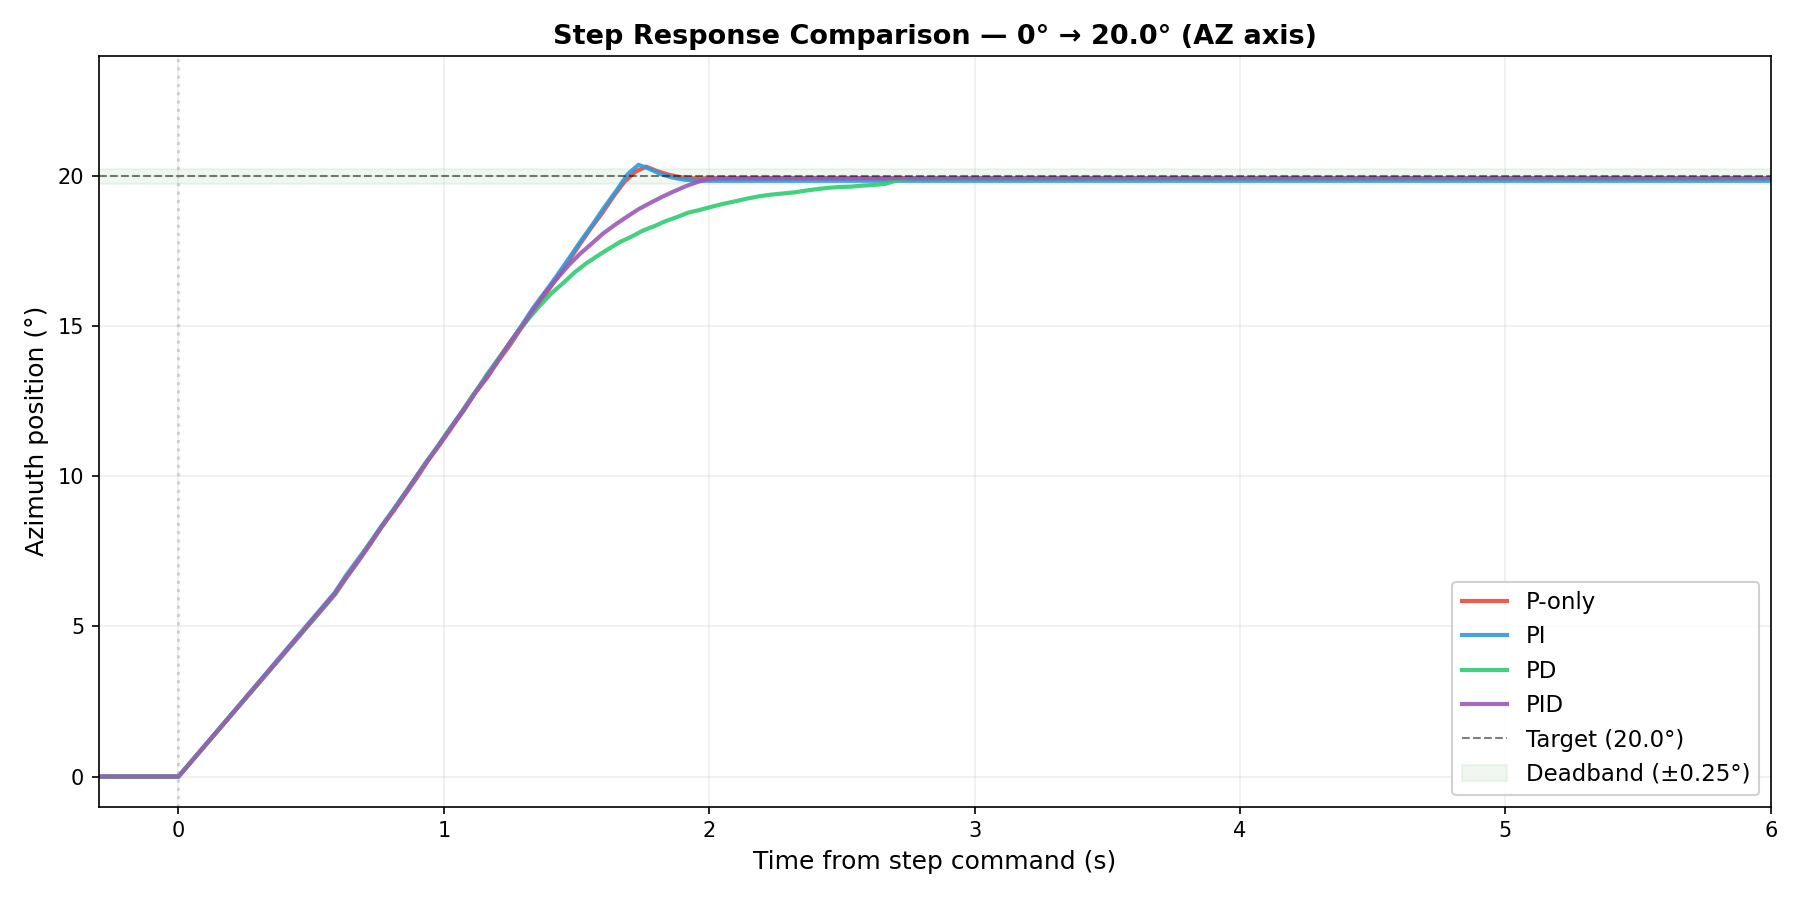
\includegraphics[width=0.8\textwidth]{figures/pid_step_overlay.png}
    \caption{PID step response overlay: 90\degree\ commanded step, actual trajectory, and error signal. Settling to within 0.05\degree\ deadband in $\sim$4~s, $<$0.5\degree\ overshoot.}
    \label{fig:pid-step-overlay}
\end{figure}

\begin{figure}[H]
    \centering
    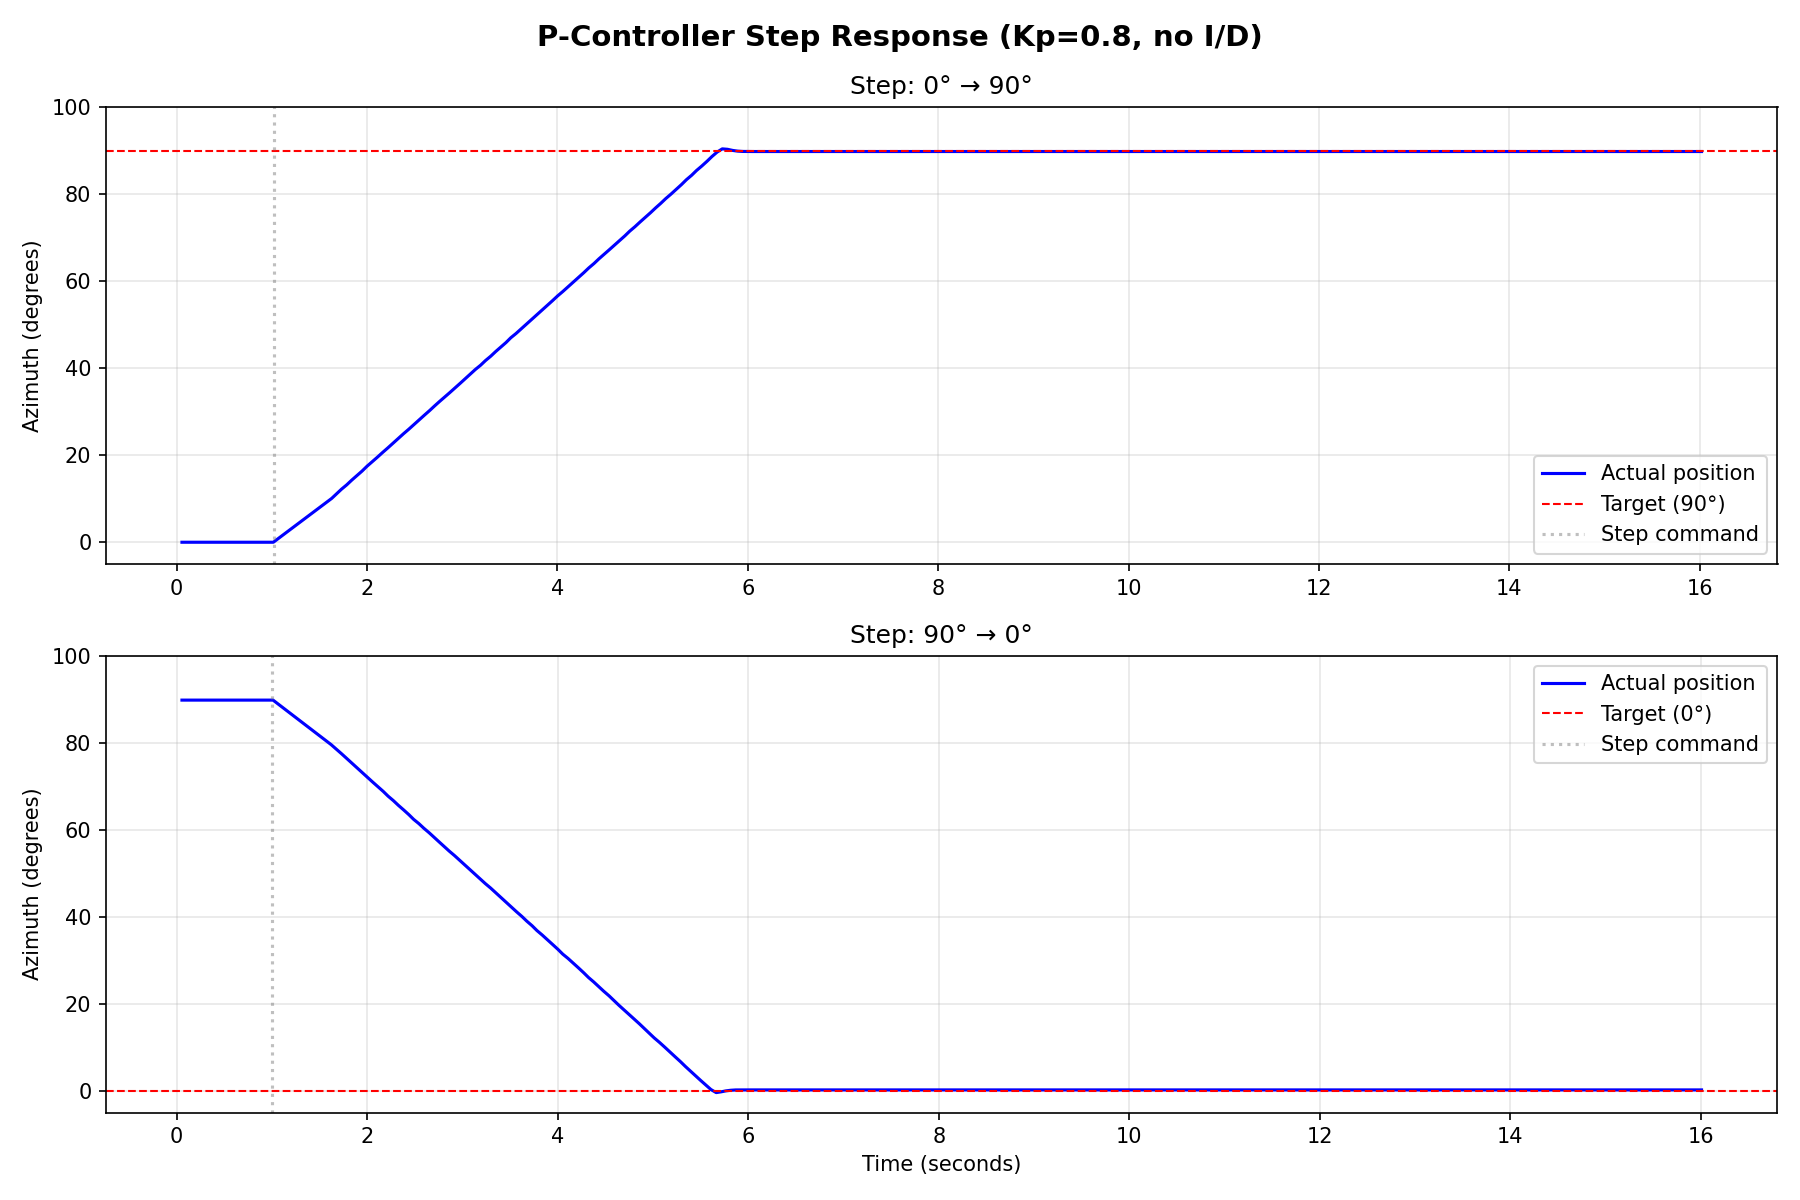
\includegraphics[width=0.8\textwidth]{figures/p_controller_step_response.png}
    \caption{PID vs. P-only step response, same 90\degree\ step. The integral term eliminates the $\sim$2\degree\ steady-state error left by the proportional controller alone.}
    \label{fig:p-controller-step}
\end{figure}

\begin{figure}[H]
    \centering
    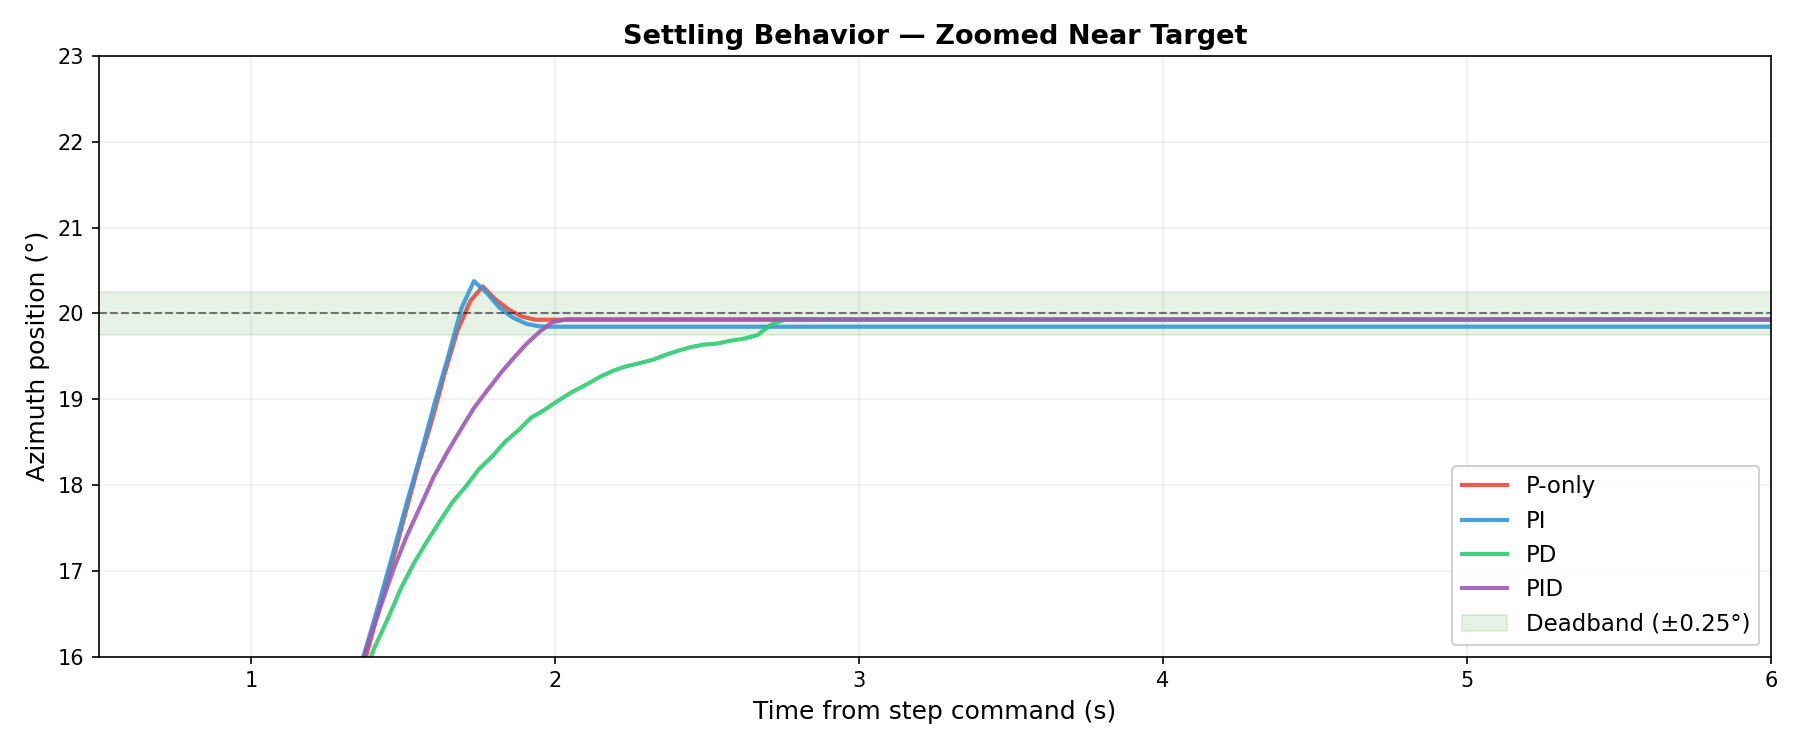
\includegraphics[width=0.8\textwidth]{figures/pid_settling_zoom.png}
    \caption{PID settling detail (zoomed): $\pm$1\degree\ around the setpoint for the last second of the step. Deadband band at $\pm$0.05\degree\ visible.}
    \label{fig:pid-settling-zoom}
\end{figure}

\begin{figure}[H]
    \centering
    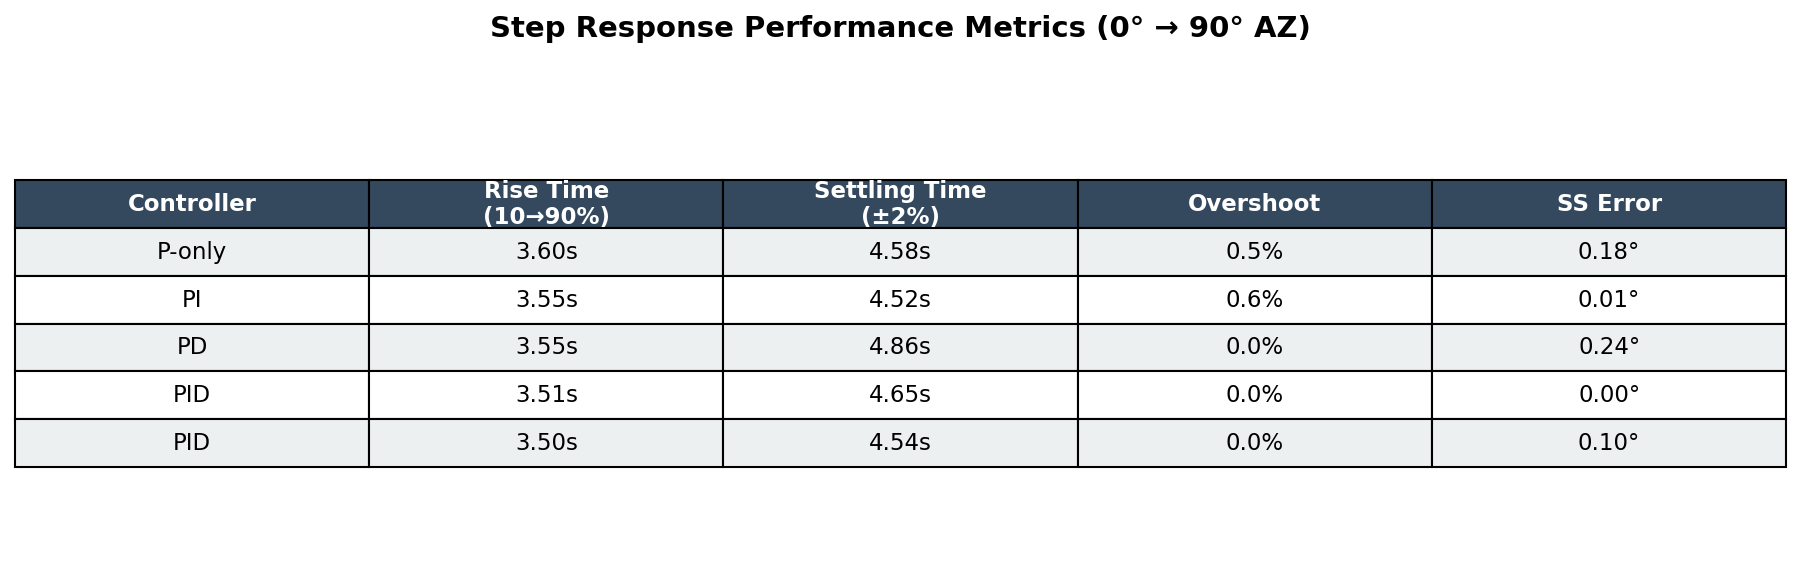
\includegraphics[width=0.7\textwidth]{figures/pid_metrics_table.png}
    \caption{PID metrics summary table: overshoot, settling time, steady-state error per axis at three duty limits.}
    \label{fig:pid-metrics-table}
\end{figure}

\section{Quadrature Encoding}
\label{sec:quadrature}

The Hall-effect encoder on each motor shaft gives two channels A, B. 4$\times$ decode produces the 64 CPR / 244.6 AZ ticks/deg / 126.1 EL ticks/deg resolution derived in \S\ref{sec:gearing}.

The decoder is an interrupt-driven Gray-code state machine on RP2040 core 1. At the 35\degree/s peak slew (\S\ref{sec:slew-speed}), the inter-edge period on the fastest axis is $1/(35 \cdot 244.6) = 117$~$\mu$s; the measured ISR latency is $<$10~$\mu$s per edge.

\section{Homing and Calibration}
\label{sec:homing}

\textbf{EL:} ADXL345 gravity vector $\to$ drive to horizontal $\to$ zero encoder. The \code{RECAL} command re-homes during operation.

\textbf{AZ:} assume north at boot. User points the station north (guided by the phone compass on the dashboard) and confirms via the setup wizard; the \code{ZERO} command sets the current position as 0\degree.

\begin{figure}[H]
    \centering
    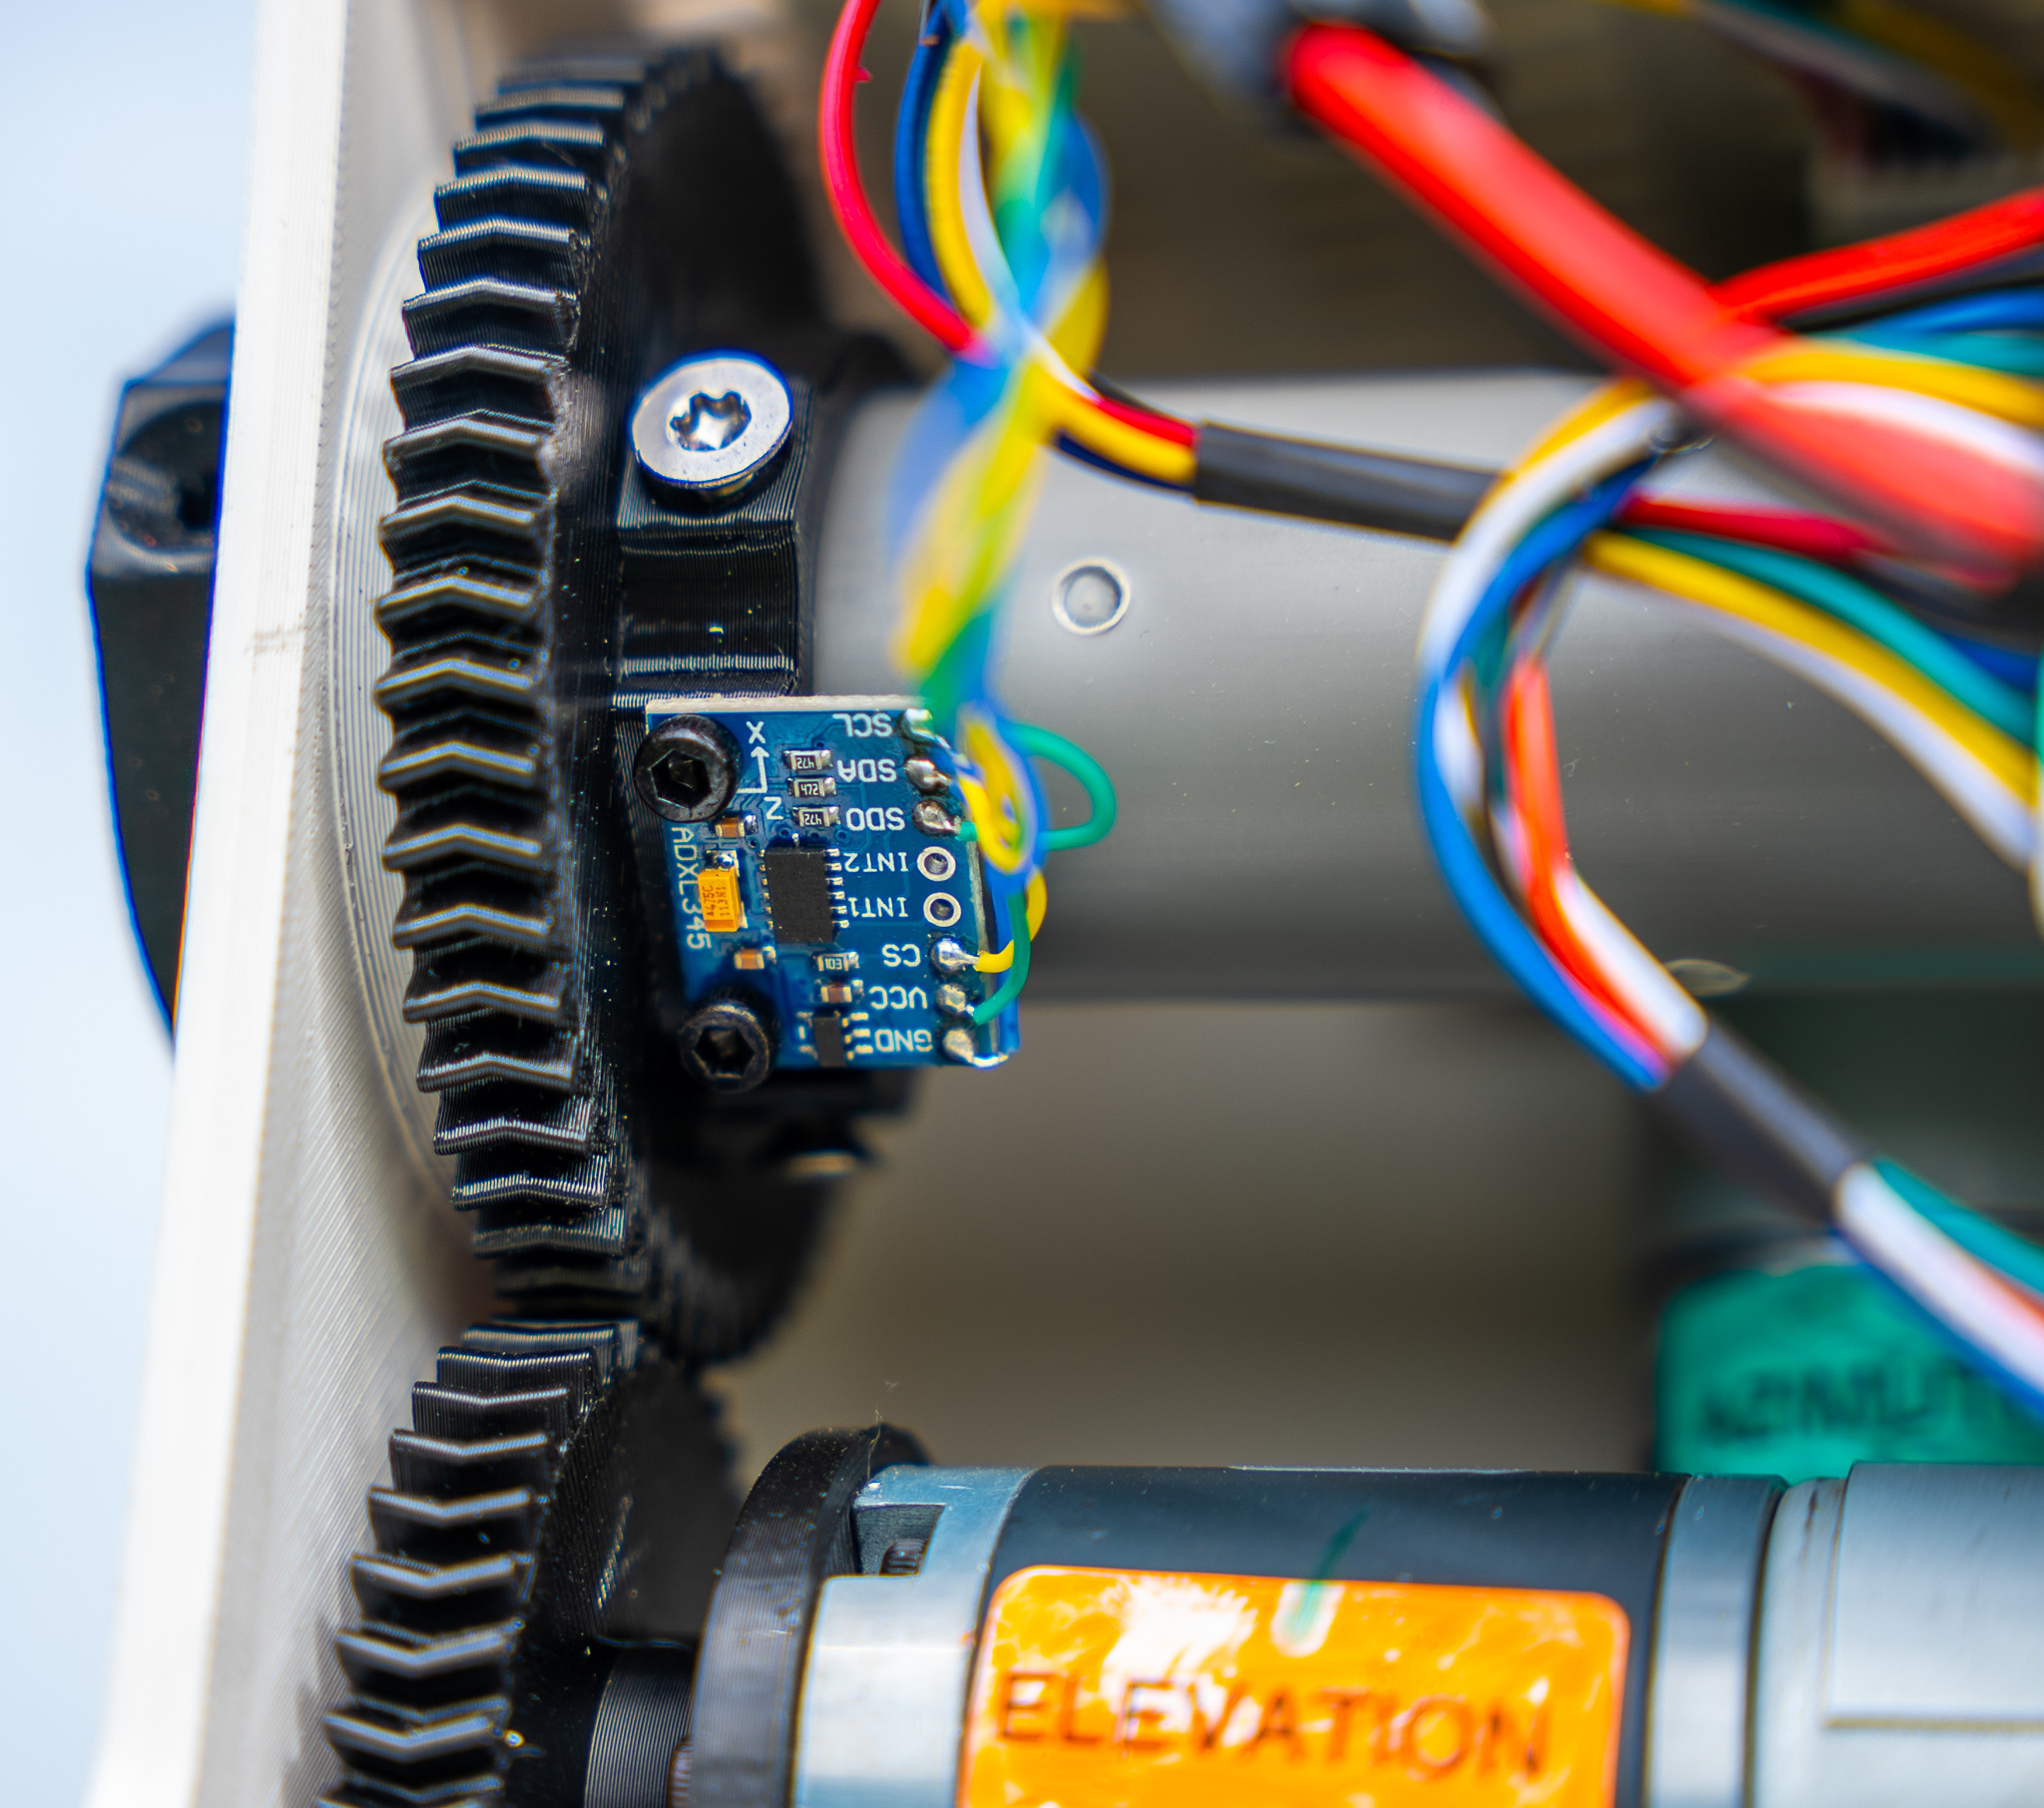
\includegraphics[width=0.55\textwidth]{photos/imu.jpg}
    \caption{ADXL345 accelerometer breakout used for EL homing, mounted on the elevation frame with SPI0 wiring to the MotorPCB (MISO GP4, CSn GP5, SCK GP6, MOSI GP7).}
    \label{fig:imu}
\end{figure}

\section{Safety}
\label{sec:safety}

\begin{itemize}
    \item \textbf{Runaway detection}: e-stop if position exceeds soft limits by 50\degree.
    \item \textbf{Shortest-path wrapping}: 350\degree $\to$ 10\degree\ takes a 20\degree\ path rather than 340\degree; re-centres the encoder after settling near $\pm$360\degree.
    \item \textbf{8~s hardware watchdog}, including during the EL homing loop.
\end{itemize}

\section{EasyComm Implementation}
\label{sec:easycomm}

Standard commands: \code{AZ}/\code{EL} set/get, \code{PARK}, \code{STOP}, \code{VE}, \code{GS}/\code{GE}.
Custom extensions: \code{RESET}, \code{RECAL}, \code{MONITOR}, \code{TICKS}, \code{ZERO}, \code{GAINS}, \code{IMU}.

Custom commands are invisible to hamlib, so compatibility with \code{rotctld}, GPredict, and the \code{satnogs-client} rotator path is maintained. The full EasyComm + extensions parser is implemented in \file{satnogs\_protocol.cpp} ($\sim$250 lines of C++).

\section{RF HAT Firmware}
\label{sec:rf-hat-firmware}

Binary protocol: COBS framing + CRC-16/CCITT-FALSE over UART 115200.

Key message types:
\begin{itemize}
    \item \code{SELECT\_RADIO} (0x40) --- switch UHF/VHF CC1200.
    \item \code{READ/WRITE\_REG}, \code{READ/WRITE\_EXT} --- CC1200 register access.
    \item \code{PROFILE\_BEGIN/CHUNK/APPLY} --- SmartRF profile loading (chunked, no reflash needed).
    \item \code{SET\_STREAMING} --- enable/disable continuous RX packet forwarding.
    \item \code{SET\_SERIAL\_MODE} (0x35) --- enable PIO-based serial bitstream capture.
    \item \code{TX\_WRITE/SEND} --- load FIFO + transmit.
    \item \code{BUZZER} (0x50) --- trigger patterns (ready, AOS, LOS, packet, error).
    \item \code{PING/PONG} --- connectivity test.
    \item \code{EVT\_RX\_DATA} (0xE0) --- asynchronous received data (firmware$\to$Pi, both FIFO and serial modes).
\end{itemize}

CC1200 SPI driver: SPI1 = UHF (GP10--13), SPI0 = VHF (GP16--19), 5~MHz clock. Each on a separate SPI peripheral --- no bus contention.

4$\times$ WS2812B NeoPixels on GP4. Non-blocking buzzer tone sequencer on GP5 (hardware PWM via NPN/MOSFET gate).

\subsection{CC1200 Serial Mode and AX.25 G3RUH Decoding}
\label{sec:serial-mode}

The CC1200's default FIFO mode requires sync-word detection before delivering data. G3RUH scrambling~\cite{g3ruh-scrambler} randomises the bitstream before transmission, so the over-the-air bytes do not contain the pre-scrambling sync word and FIFO mode will either miss the frame or false-trigger on scrambled noise. Undocumented framing hits the same wall. The firmware therefore implements a synchronous serial receive mode using the RP2040's PIO (Programmable I/O) peripheral.

The CC1200 is reconfigured for synchronous serial output (\code{PKT\_FORMAT=0x01}, \code{FIFO\_EN=0}, \code{SYNC\_MODE=0x00}) with GPIO0 carrying the demodulated bitstream and GPIO2 carrying the recovered bit clock. The internal demodulator runs continuously, outputting every demodulated bit.

A 3-instruction PIO program (\file{serial\_rx.pio.h}) captures the bitstream into the CPU via autopush:

\begin{verbatim}
.wrap_target
    wait 1 pin 2    ; SERIAL_CLK rising edge
    in pins, 1      ; shift in SERIAL_RX
    wait 0 pin 2    ; SERIAL_CLK falling edge
.wrap
\end{verbatim}

The PIO is gated by the CC1200 clock output, so no baud-rate setup is needed on the RP2040 side.

In blind mode the CC1200 outputs samples at $\sim$7--8$\times$ the configured symbol rate. The firmware measures this ratio at startup (PIO word count over 100~ms divided by the expected symbol rate), then an edge-triggered resampler extracts data bits at the midpoint of each symbol period.

Two serial sub-modes are selected via the \code{MSG\_SET\_SERIAL\_MODE} body byte:

\begin{enumerate}
    \item \textbf{Mode 1 --- raw serial.} Demodulated bytes go to a 256-byte ring buffer, forwarded to the Pi as \code{EVT\_RX\_DATA} every 50~ms or 32~bytes. Used for blind capture of unknown framing.
    \item \textbf{Mode 2 --- AX.25 G3RUH decode.} Each resampled bit is fed through a three-stage pipeline implemented in \file{ax25\_decode.c}:
    \begin{itemize}
        \item \textbf{G3RUH descrambler}: 17-bit LFSR, polynomial $x^{17} + x^{12} + 1$, reverses the AMSAT scrambler.
        \item \textbf{NRZ-I decoder}: differential to absolute.
        \item \textbf{HDLC deframer}: 0x7E flag detection, bit-stuffing removal after five consecutive ones, LSB-first byte assembly, CRC-16/CCITT check (poly 0x8408, residual 0xF0B8). Minimum valid frame 17~bytes (14 address + 1 control + 2 FCS).
    \end{itemize}
    CRC-valid frames go up as \code{EVT\_RX\_DATA} with \code{type=0x01}; raw bytes are forwarded in parallel for diagnostics.
\end{enumerate}

\code{station.py} selects serial mode automatically for satellites at $\geq$4800~bps FSK/GFSK (likely G3RUH), and FIFO mode with the AX.100 sync word 0x930B51DE for lower-rate satellites using the GOMspace NanoCom format.

\begin{figure}[H]
    \centering
    % TODO: draw diagram
    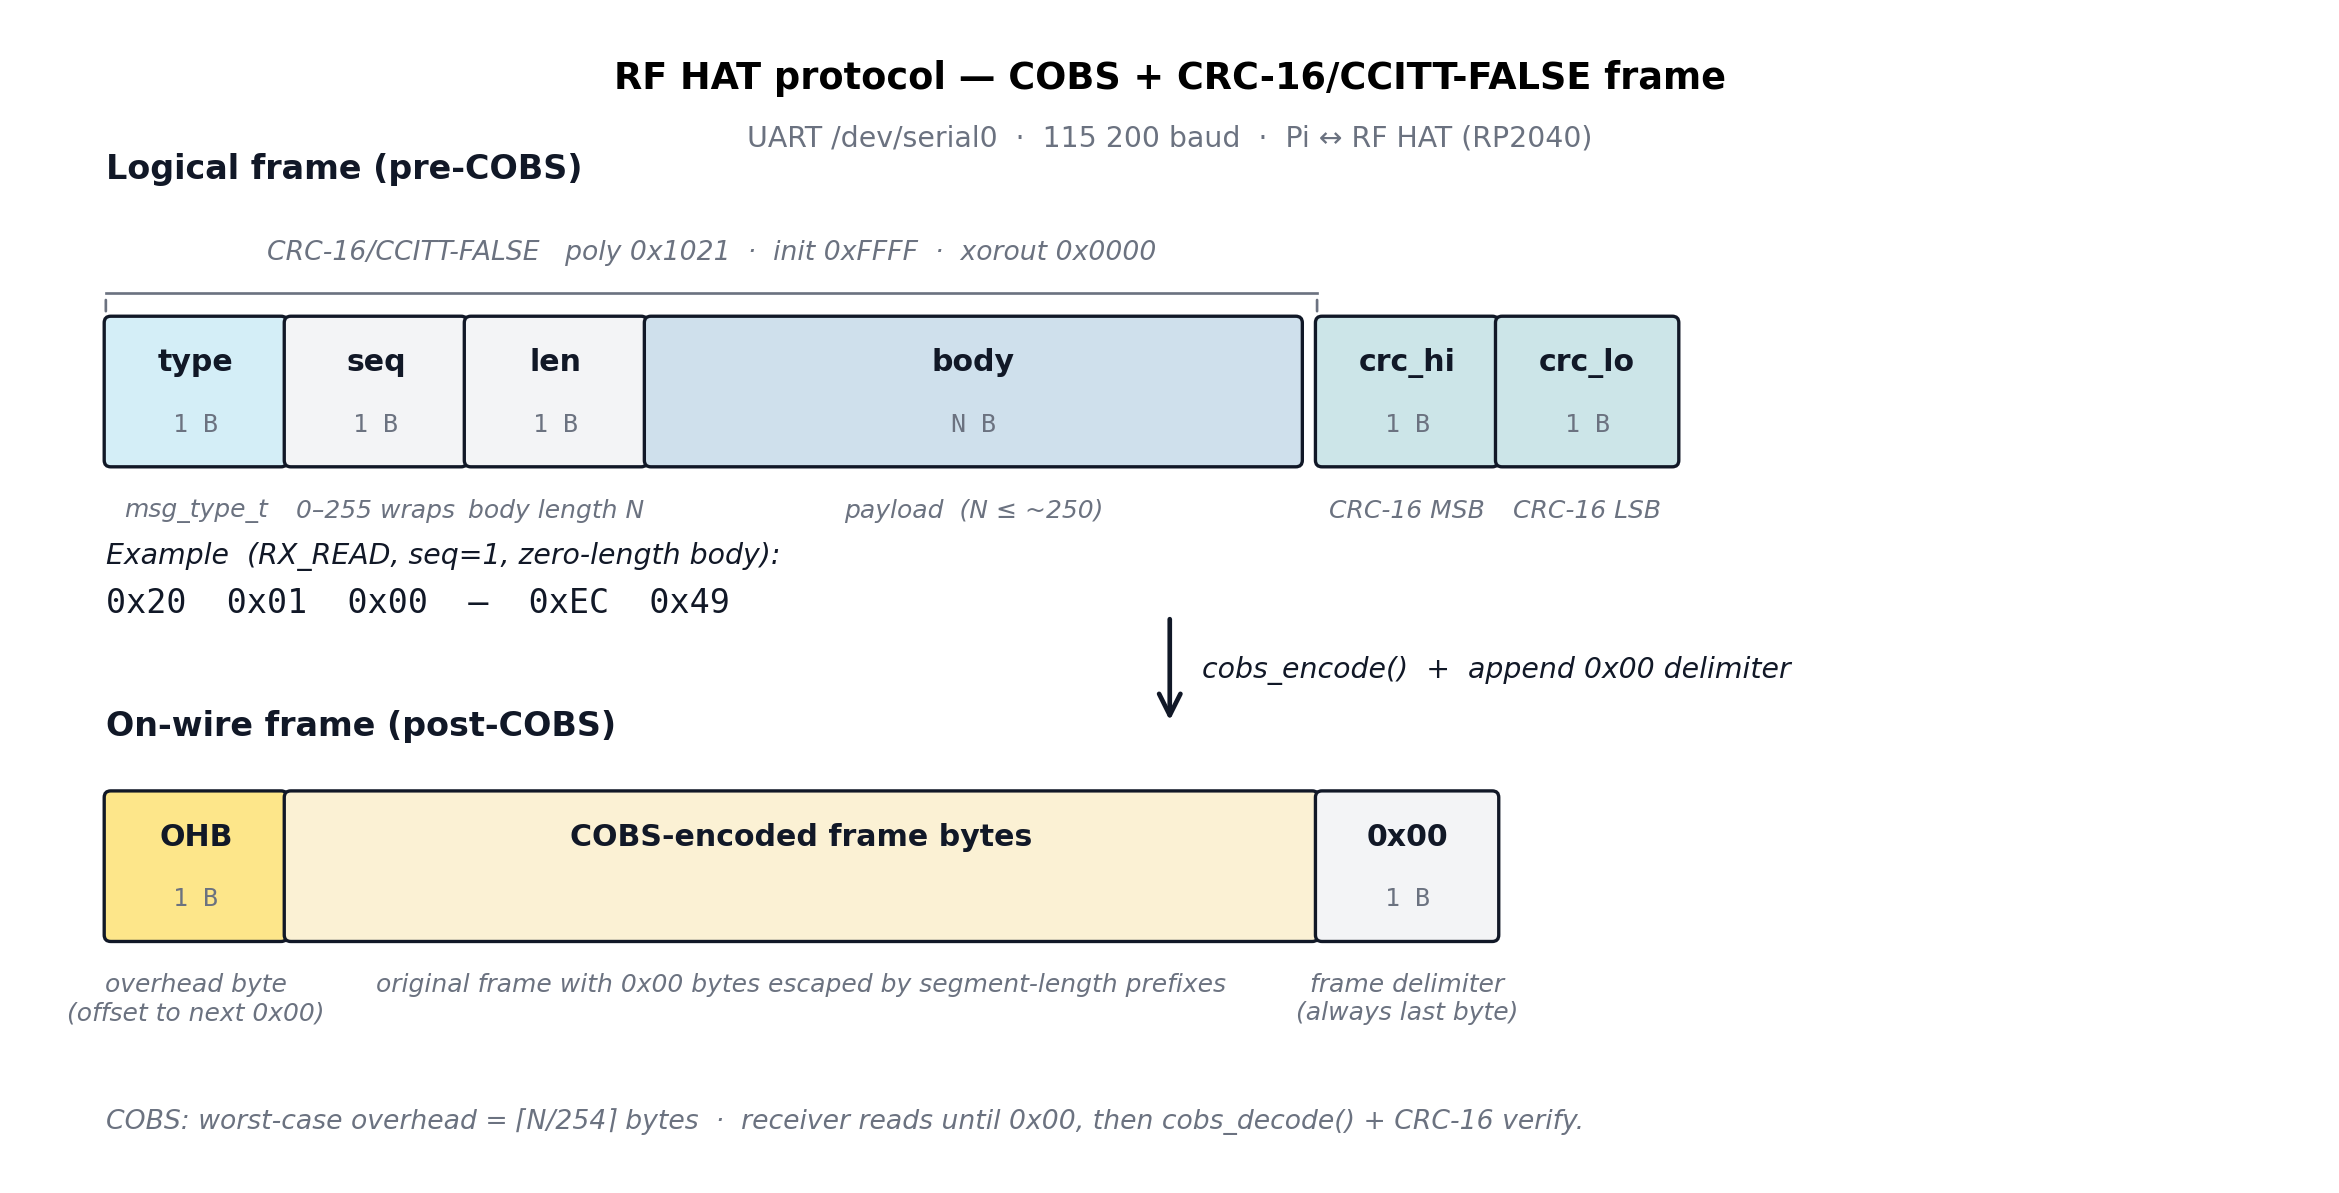
\includegraphics[width=0.85\textwidth, height=4cm, keepaspectratio]{figures/cobs_frame_diagram.png}
    \caption{COBS frame structure: \code{[type | seq | len | payload\ldots(len bytes) | crc16\_hi | crc16\_lo]} encoded with Consistent Overhead Byte Stuffing, terminated by a 0x00 delimiter. Response type byte has bit 7 set (\code{type | 0x80}). CRC-16/CCITT-FALSE (poly 0x1021, init 0xFFFF) computed over \code{[type | seq | len | payload]} before COBS encoding.}
    \label{fig:cobs-frame}
\end{figure}

\section{Raspberry Pi Software Stack}
\label{sec:pi-stack}

\subsection*{station.py}

Main orchestration, two modes: manual (\code{--sat "ISS"} or auto-pick the next pass) and daemon (systemd service, waits for GPS from the dashboard, loops passes continuously). During a pass:

\begin{enumerate}
    \item Fetch TLEs from CelesTrak, compute trajectory with PyEphem.
    \item Pre-position rotator to AOS azimuth.
    \item Stream AZ/EL to \code{rotctld} at 10~Hz.
    \item Configure the CC1200 for the satellite's frequency/modulation from the local profile DB, falling back to the SatNOGS DB API.
    \item Apply Doppler correction at 2~Hz --- \code{FREQOFF} register for normal updates, full \code{FREQ} rewrite for large jumps.
    \item Drain RX packets and log telemetry (position, RSSI, freq, Doppler, range) to CSV at 5~Hz.
    \item Write \file{\textasciitilde/.station\_status.json} at $\sim$5~Hz for the dashboard.
\end{enumerate}

Scan mode cycles through visible satellites near peak elevation with a 30~s dwell each.

\subsection*{rf\_hat.py --- CC1200Link}

Threaded serial interface: COBS framing, CRC verification, SmartRF parsing, frequency calculation across 136--960~MHz, modulation config (2-FSK, 2-GFSK, 4-FSK, OOK), per-satellite radio configuration.

\subsection*{dashboard.py --- HTTPS web dashboard}

The dashboard is a self-contained HTTPS server built on the Python standard library only (no Flask, no npm). It serves a single-page app at \url{https://<pi-ip>:5000} for phone- or laptop-based field use.

HTTPS is required because the browser Geolocation API needs a secure context. A self-signed TLS certificate is auto-generated on first run (\file{\textasciitilde/.station\_ssl/}); the user accepts the browser warning on first visit.

Three pages:
\begin{itemize}
    \item \textbf{Track} --- sky plot, live AZ/EL (commanded vs. actual), RSSI, packet count, Doppler, pass progress. Upcoming passes come from TLE propagation enriched with SatNOGS DB frequency and modulation data. Filters: band (UHF/VHF), minimum elevation, CC1200-compatible modulation.
    \item \textbf{Control} --- numeric AZ/EL goto, six preset positions (park, zenith, N/E/S/W at 45\degree\ EL), and a CC1200 debug panel (MARC state, FIFO levels, overflow count, raw register values).
    \item \textbf{Settings} --- GPS entry, WiFi configuration, station parameters, and the setup wizard.
\end{itemize}

The setup wizard has five steps: (1) phone GPS $\to$ Pi, (2) point the station north using the phone compass and confirm with \code{ZERO}, (3) attach the antenna (the station is level from IMU homing), (4) select receiver type, (5) ready. Tracking begins automatically after step 5.

\begin{figure}[H]
    \centering
    % TODO: capture phone screenshot
    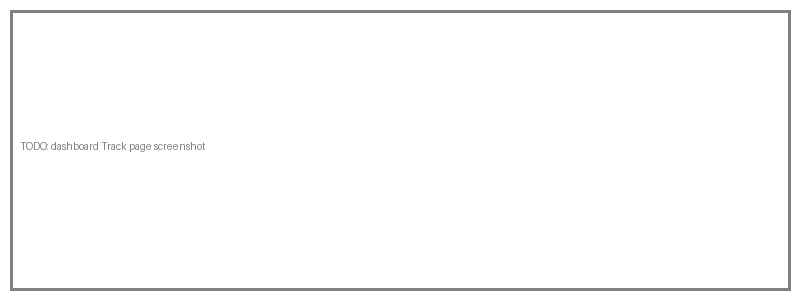
\includegraphics[width=0.45\textwidth, height=8cm, keepaspectratio]{figures/dashboard_track_page.png}
    \caption{Dashboard Track page on phone: sky plot with satellite trajectory, live AZ/EL commanded vs. actual, RSSI bar, Doppler offset, pass timer, and filtered satellite list enriched from SatNOGS DB.}
    \label{fig:dashboard-track}
\end{figure}

\begin{figure}[H]
    \centering
    % TODO: capture phone screenshot
    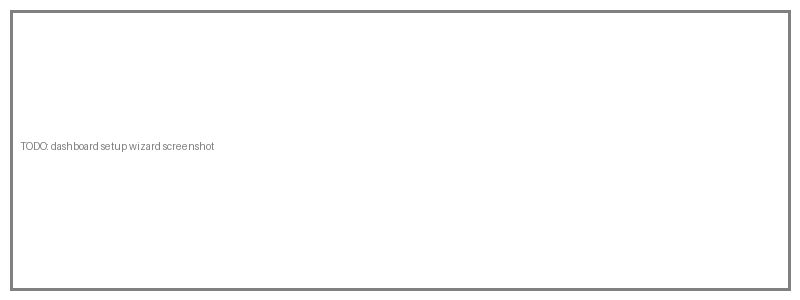
\includegraphics[width=0.45\textwidth, height=8cm, keepaspectratio]{figures/dashboard_setup_wizard.png}
    \caption{Dashboard Settings page showing the five-step setup wizard: phone GPS $\to$ point-north compass $\to$ antenna attach $\to$ receiver selection $\to$ ready.}
    \label{fig:dashboard-wizard}
\end{figure}

\subsection*{Systemd services and auto-start}

Three systemd services run the station autonomously after boot:

\begin{enumerate}
    \item \file{rotctld.service} --- hamlib rotator daemon, model 204, listening on TCP 4533. Restarts automatically if the USB connection to the rotator Pico is interrupted.
    \item \file{dashboard.service} --- HTTPS dashboard on port 5000. Starts immediately on boot.
    \item \file{station.service} --- station controller in daemon mode. Waits for \file{station.conf} (written by the dashboard when the user provides GPS), then continuously fetches TLEs, computes passes, and tracks them in a loop.
\end{enumerate}

A setup script (\file{Pi/services/setup-pi.sh}) configures a fresh Raspberry Pi with all dependencies, UART configuration (\code{enable\_uart=1}, \code{dtoverlay=disable-bt}), a WiFi rfkill workaround (Debian Trixie blocks WiFi by default), and service installation. The script is idempotent.

\subsection*{SatNOGS network integration}

The station is registered as station 4712 (``Aether-Basestation'') on \url{network.satnogs.org}. SiDS telemetry submission to \url{db.satnogs.org} is verified (HTTP 201 OK).

Because the CC1200 emits decoded packets rather than raw IQ, \code{satnogs-client} (GNU~Radio + SoapySDR) cannot be used as-is; frames are submitted directly to the SatNOGS DB over the SiDS API. The station therefore appears ``offline'' on the network map (no job-polling heartbeat) but still contributes telemetry on decode. The rationale for this trade-off is covered in \S\ref{sec:problem-statement} and \S\ref{sec:cc1200-deviation}.

\begin{figure}[H]
    \centering
    % TODO: draw diagram
    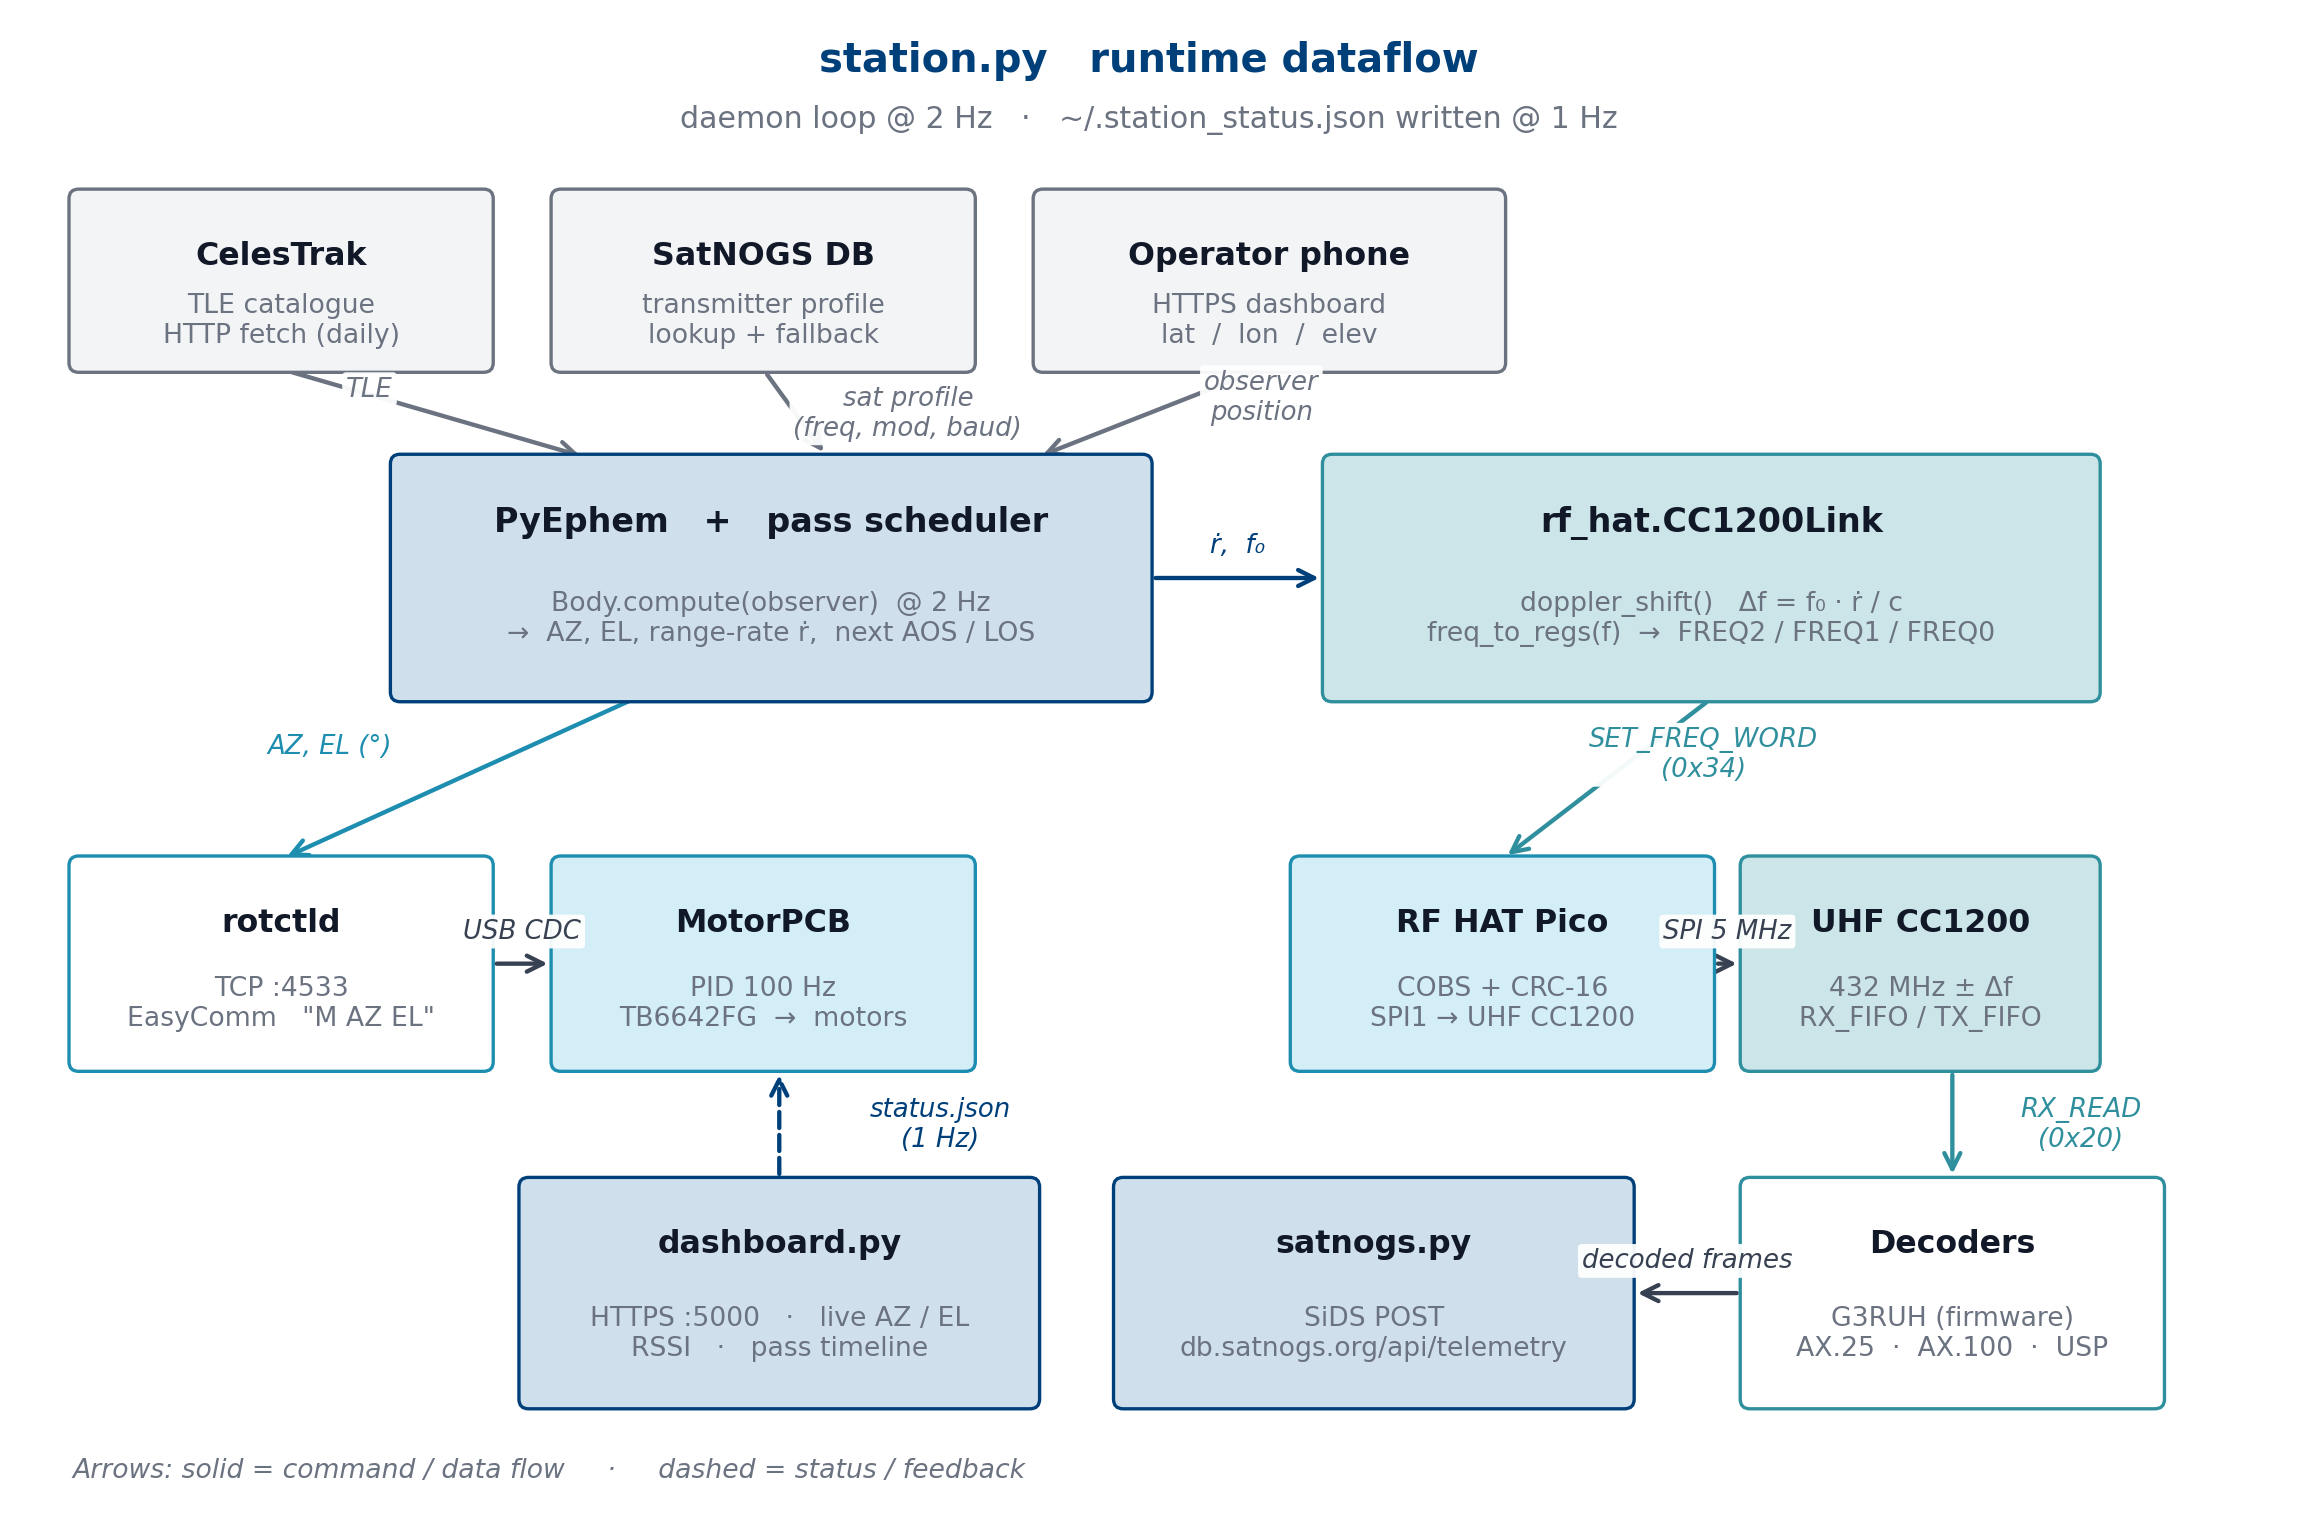
\includegraphics[width=0.95\textwidth, height=6cm, keepaspectratio]{figures/station_dataflow_diagram.png}
    \caption{\code{station.py} data flow: CelesTrak TLE $\to$ PyEphem propagation $\to$ AZ/EL setpoints at 10~Hz $\to$ \code{rotctld} (TCP 4533) $\to$ MotorPCB (USB CDC, EasyComm). In parallel: satellite profile lookup (local DB $\to$ SatNOGS DB API fallback) $\to$ CC1200Link SmartRF load; during pass, Doppler FREQOFF update at 2~Hz $\to$ CC1200; RX packets/RSSI drained over UART, logged to CSV at 5~Hz, and pushed to \file{\textasciitilde/.station\_status.json} at 5~Hz for the dashboard.}
    \label{fig:station-dataflow}
\end{figure}

\section{Field Deployment Workflow}
\label{sec:field-deployment}

The deployment sequence, measured at $\sim$4~minutes from unpacking to first tracked pass across the three field sessions:

\begin{enumerate}
    \item Place on tripod, point north, connect 24~V.
    \item Pi boots, EL homes via IMU, services start ($\sim$60~s).
    \item Phone joins the Pi WiFi (or the captive-portal provisioner).
    \item Dashboard $\to$ ``Use My GPS'' $\to$ station location set.
    \item Setup wizard: confirm north, attach antenna, select receiver type.
    \item Auto-tracking begins; dashboard shows live status.
    \item End of session $\to$ \code{PARK} $\to$ shutdown $\to$ wait 10~s $\to$ unplug.
\end{enumerate}

No laptop or SSH is used in the field.

\begin{figure}[H]
    \centering
    % TODO: draw diagram
    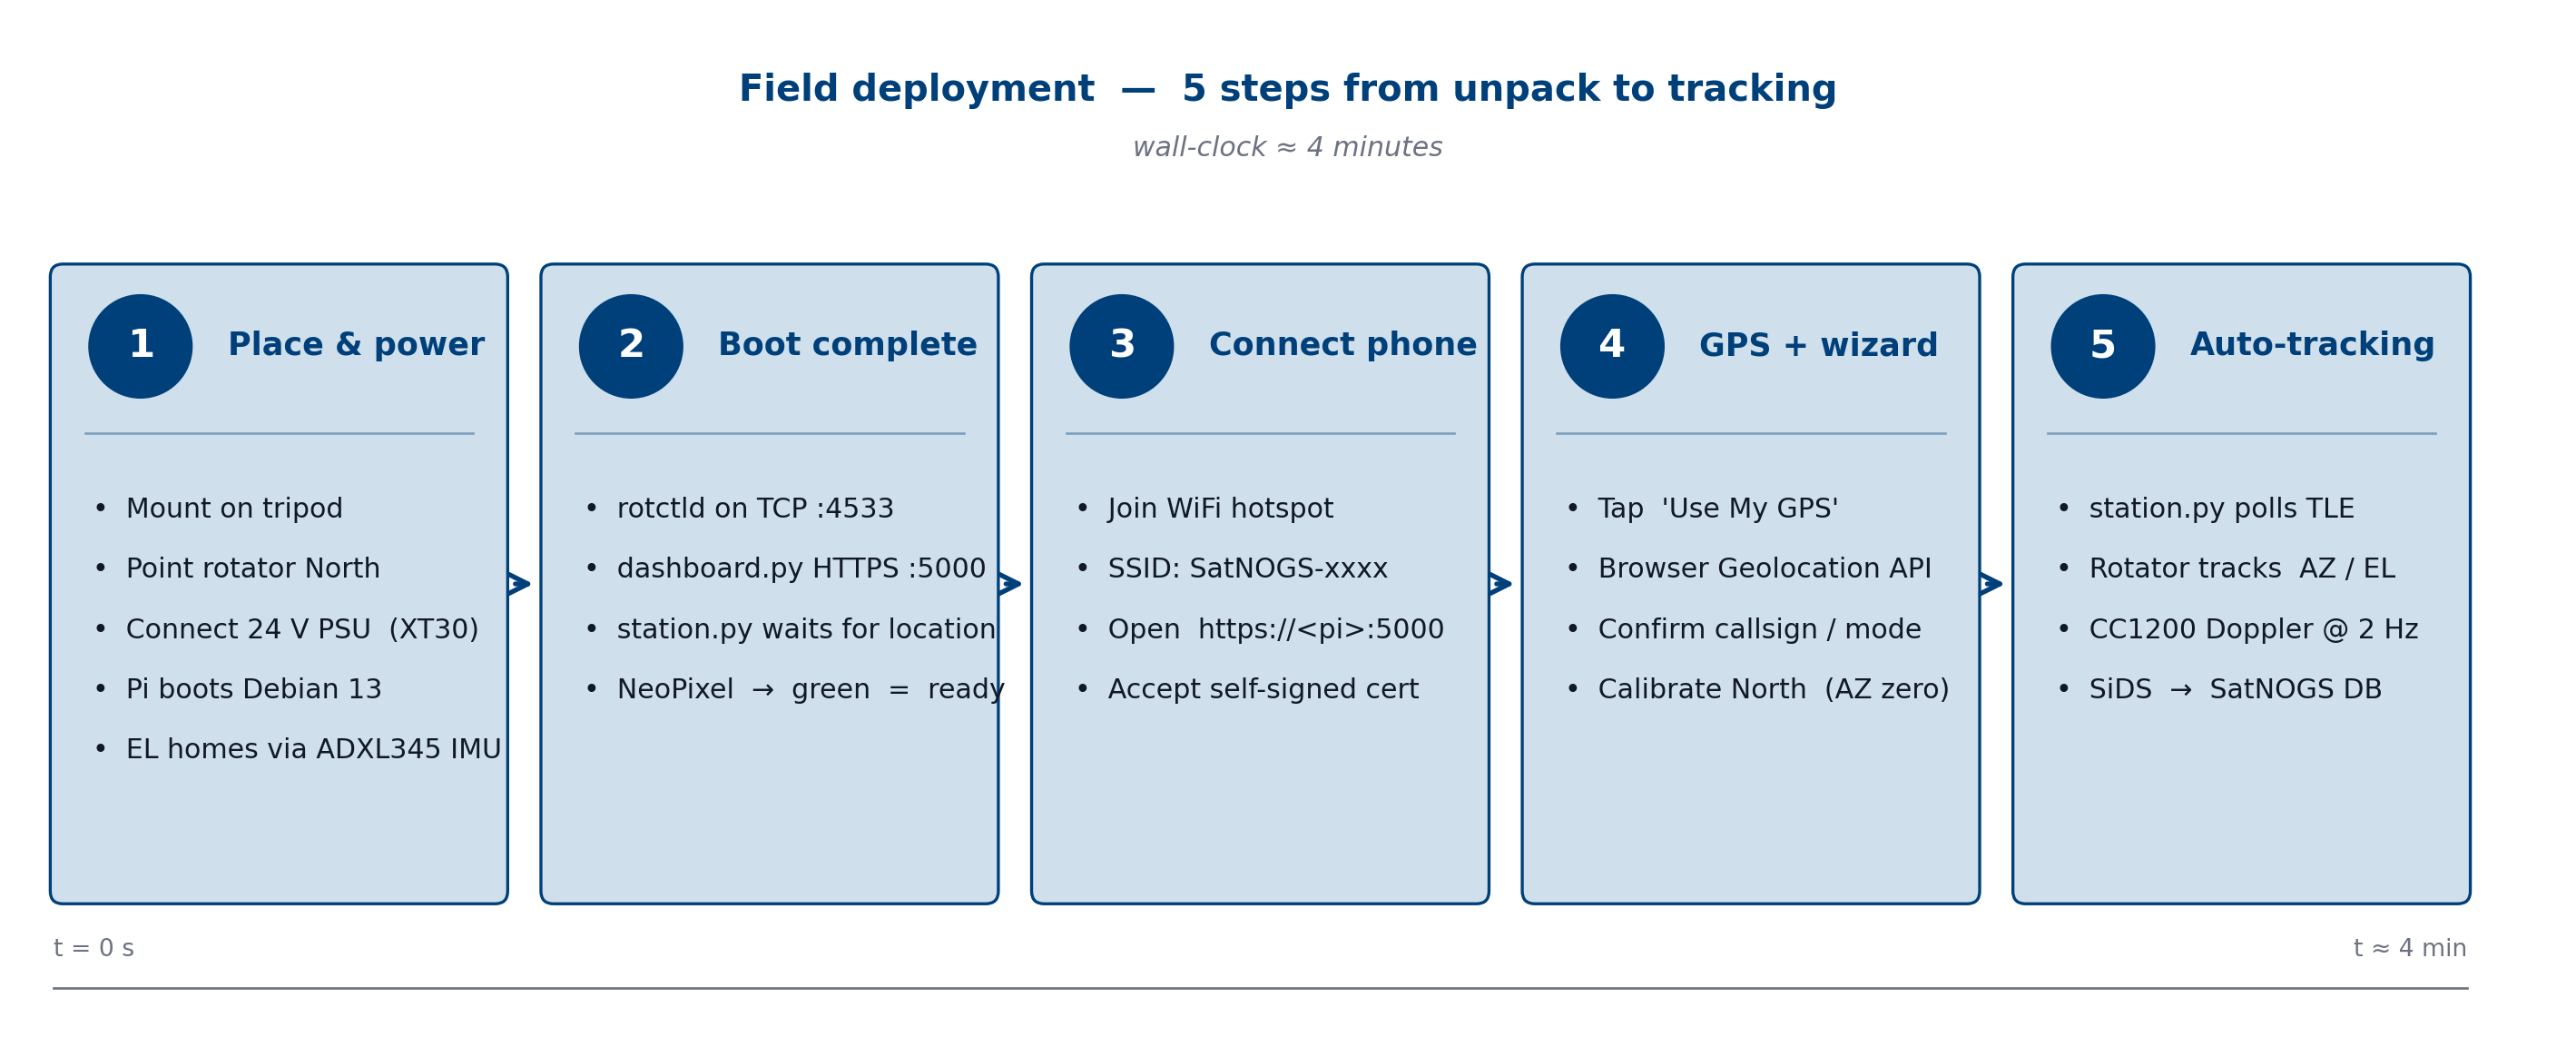
\includegraphics[width=0.85\textwidth, height=5cm, keepaspectratio]{figures/field_deployment_workflow.png}
    \caption{Field deployment workflow: (1) place on tripod, connect 24~V; (2) Pi boots, EL homes via IMU; (3) phone joins Pi WiFi (or captive-portal provisioning); (4) dashboard $\to$ ``Use My GPS''; (5) setup wizard $\to$ tracking begins.}
    \label{fig:field-deployment}
\end{figure}

\begin{figure}[H]
    \centering
    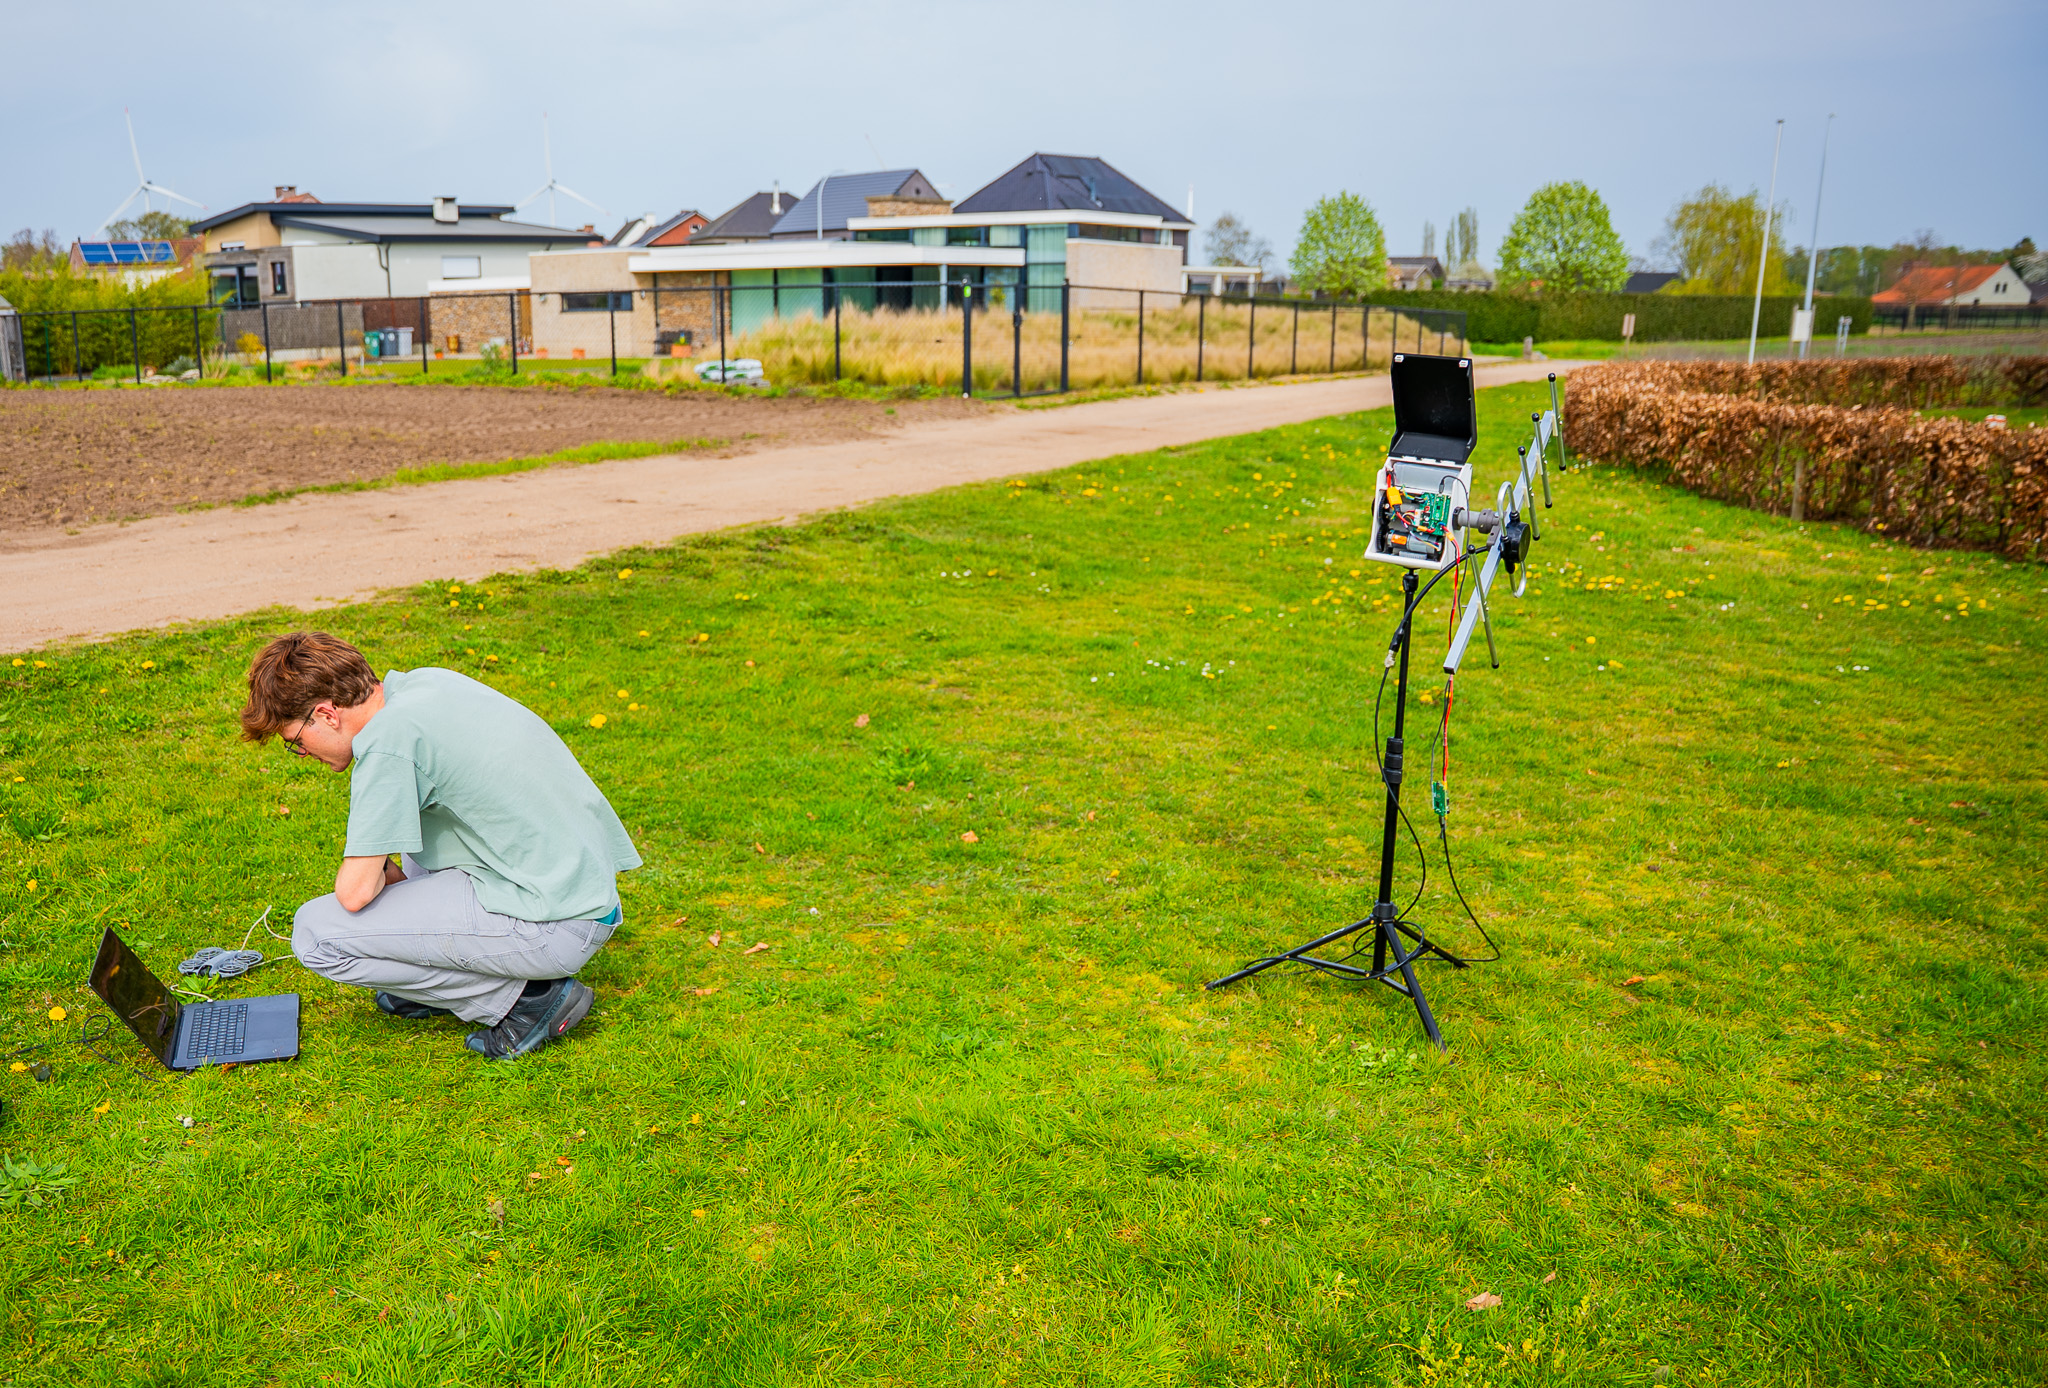
\includegraphics[width=0.7\textwidth]{photos/station_whole_setup.jpg}
    \caption{Station deployed in the field: tripod, rotator, Yagi on EL axis, 24~V bench supply via extension cord. Photo from the April 9 session.}
    \label{fig:station-deployed}
\end{figure}

\begin{figure}[H]
    \centering
    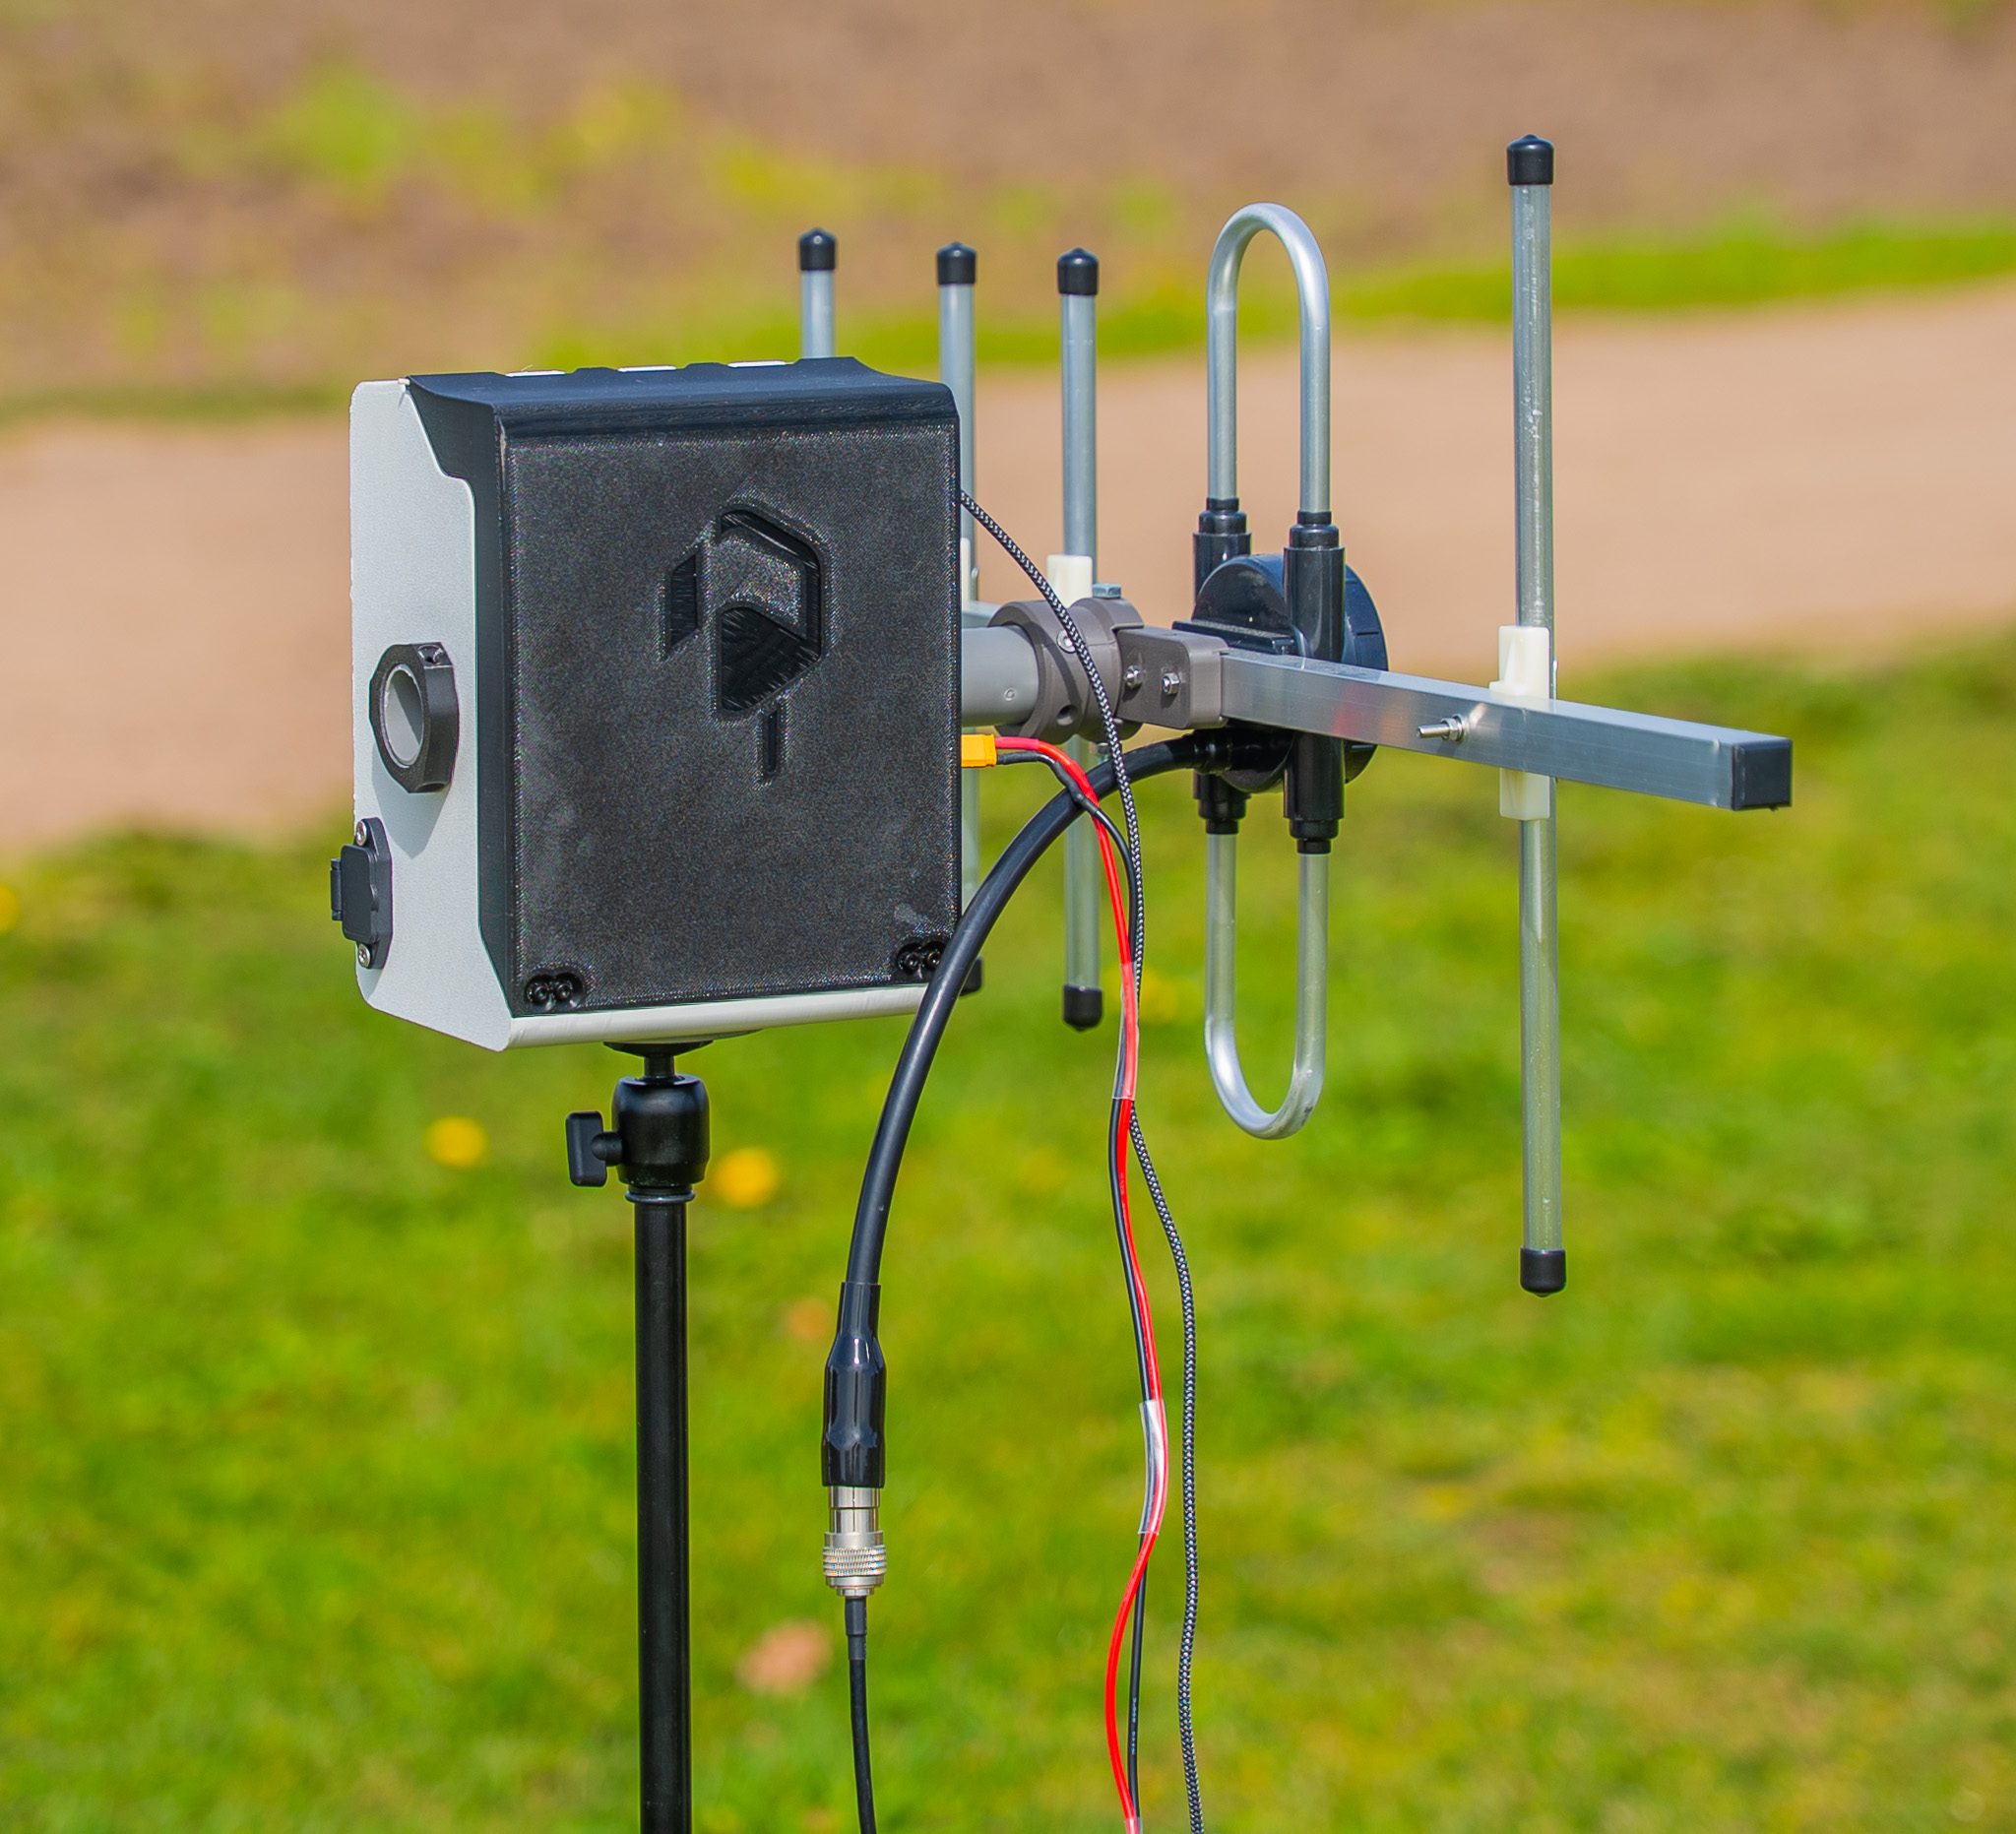
\includegraphics[width=0.6\textwidth]{photos/station_closeup.jpg}
    \caption{Close-up of the deployed station showing the rotator + Yagi feed + RF HAT cable routing.}
    \label{fig:station-closeup}
\end{figure}

% ══════════════════════════════════════════════════════════════════════════════
\chapter{Results and Validation}
\label{ch:results}
% ══════════════════════════════════════════════════════════════════════════════

\section{Slew Speed}
\label{sec:slew-speed}

Slew speed was measured on a single axis, unloaded, at 24~V supply, by commanding the rotator to traverse 360\degree\ at a fixed PWM duty and timing the traverse with the onboard encoder tick counter. Four duty levels were tested. Raw data and per-run encoder-derived rates are listed in Appendix~\ref{app:pid}.

\begin{table}[H]
    \centering
    \begin{tabular}{lll}
        \toprule
        Duty (\%) & Speed (\degree/s) & 360\degree\ time (s) \\
        \midrule
        35 & 11.2 & 32.1 \\
        55 & 18.9 & 19.0 \\
        75 & 26.9 & 13.4 \\
        95 & 35.0 & 10.3 \\
        \bottomrule
    \end{tabular}
    \caption{Slew-speed measurements, unloaded, 24~V supply.}
\end{table}

Linear regression over the four measured points gives slope 0.40\degree/s per \% duty, $R^2 > 0.99$. 100\,\% duty was tested separately and trips the TB6642FG overcurrent protection on motor stall, so it is not included in the fit. The 35\degree/s ceiling at 95\,\% duty exceeds the total angular rate $\dot{\theta}_{\max} \approx 1.1$\degree/s derived in \S\ref{sec:orbital-mechanics} by a factor of approximately 32. It does not cover the instantaneous \textit{azimuth} rate during near-zenith passes (which can exceed 10\degree/s for a few seconds); \S\ref{sec:tracking-accuracy} reports the resulting AZ tracking error during such passes.

\section{PID Step Response}
\label{sec:pid-step}

With the deployed gains ($K_p = 0.15$, $K_i = 0.03$, $K_d = 0.02$, duty-filter $\alpha = 0.15$, max duty 0.95; \S\ref{sec:rotator-pid}) a 90\degree\ commanded step settles to within the 0.05\degree\ deadband in approximately 4~s, with overshoot below 0.5\degree. The settling time decomposes as: slew-limited traverse of 90\degree\ at 35\degree/s peak rate = $90/35 = 2.6$~s, plus roughly 1.4~s of final convergence through the duty output filter and deadband. The closed-loop bandwidth is bounded above by the duty-output filter time constant:
\begin{equation}
    \tau_\text{duty} = \frac{\Delta t}{\alpha} = \frac{0.01}{0.15} \approx 0.067~\text{s}, \qquad f_{-3\,\text{dB}} \approx \frac{1}{2\pi \tau} \approx 2.4~\text{Hz}.
\end{equation}

In practice the slew-rate limit sets the large-signal response time; the 2.4~Hz figure applies to small-signal tracking above the deadband. Either is well above the $\leq$1.1\degree/s total angular rate of a 400~km LEO pass (\S\ref{sec:orbital-mechanics}).

\begin{figure}[H]
    \centering
    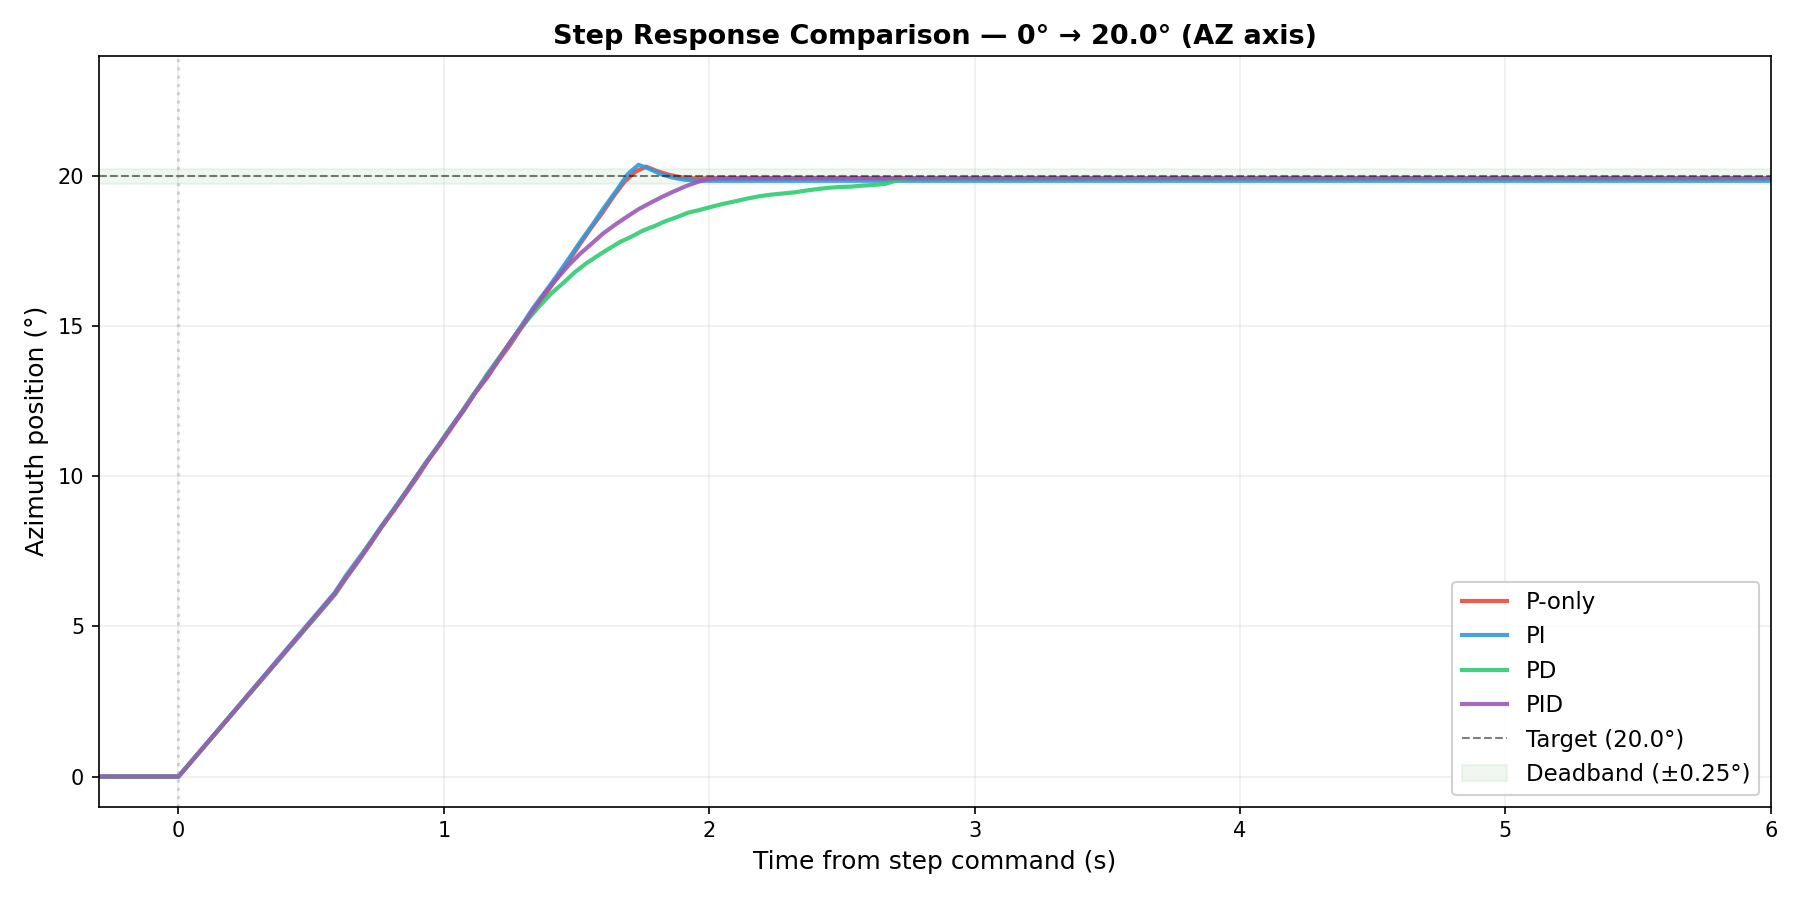
\includegraphics[width=0.8\textwidth]{figures/pid_step_overlay.png}
    \caption{PID step response for a 90\degree\ commanded step.}
\end{figure}

\section{Satellite Tracking Accuracy}
\label{sec:tracking-accuracy}

Tracking error was computed per pass from the CSV log (commanded AZ/EL from \code{station.py} pass predictor vs. actual encoder readback from the MotorPCB, sampled at 5~Hz; logs in \file{captures/20260409/pass\_logs/} and \file{captures/20260412/}). Absolute-value errors are binned by the satellite's peak-elevation category:

\begin{table}[H]
    \centering
    \begin{tabularx}{\textwidth}{lX}
        \toprule
        Scenario & Error ($|$commanded $-$ actual$|$) \\
        \midrule
        EL tracking, all passes & $<$0.5\degree\ throughout the pass \\
        AZ tracking, 20\degree--70\degree\ peak elevation & 0\degree--3\degree\ throughout the pass \\
        AZ tracking, peak elevation $>$70\degree\ (near-zenith) & 11\degree--166\degree\ during the $\sim$2--4~s zenith-crossing window; recovers to 0\degree--3\degree\ below 70\degree \\
        \bottomrule
    \end{tabularx}
    \caption{Tracking error binned by satellite peak elevation.}
\end{table}

Across passes with peak elevation in the 20\degree--70\degree\ band (the range where the Chapter~\ref{ch:background} link budget closes), both axes remain inside the Siretta Oscar 44 3-dB beamwidths (54\degree\ H-plane, 48\degree\ E-plane; \S\ref{sec:problem-statement}). The near-zenith AZ excursions exceed the 35\degree/s motor ceiling from \S\ref{sec:slew-speed} for a few seconds per pass; this is a speed-limit event, not an accuracy-limit one, and the error decreases monotonically as the satellite descends below 70\degree\ elevation.

\section{RF Devboard Validation}
\label{sec:rf-measurements}

Two devboards were connected to a host PC and exercised with \file{cc1200\_rf\_test.py}. The test script loads a bench validation SmartRF profile (2.4\,kbps 2-GFSK, 5.2\,kHz deviation, 10\,kHz channel filter; modulation index $h = 2\Delta f/f_b \approx 4.3$, chosen for robustness at short range rather than spectral efficiency, this is not the AetherSpace flight configuration, which remains to be defined once the satellite's modulation parameters are finalised), tunes both boards to a specified frequency, and runs a bidirectional packet exchange: Board\,A transmits a sequence of fixed-size payloads while Board\,B receives, then the roles are reversed. Payload matching is verified byte-for-byte.

The frequency sweep covered 430--439\,MHz in 1\,MHz steps with 50 packets per direction per frequency (1000 total). Test conditions: 1\,m board separation, dipole antennas, indoor lab, CRC-16 enabled. Table~\ref{tab:devboard-bench} shows the per-frequency results averaged over both directions.

\begin{table}[H]
    \centering
    \caption{Devboard bench test results per frequency, averaged over both directions (50 packets each). LQI lower~=~better.}
    \small
    \begin{tabular}{rrrrr}
        \toprule
        Freq (MHz) & RSSI avg (dBm) & LQI avg & Latency avg (ms) & Loss (\%) \\
        \midrule
        430 & $-$83.6$^\dagger$  & 0.4 & 103.5 & 0.0 \\
        431 & $-$103.7           & 0.3 & 103.3 & 0.0 \\
        432 & $-$102.4           & 0.5 & 103.3 & 0.0 \\
        433 & $-$103.6           & 0.4 & 104.1 & 0.0 \\
        434 & $-$103.7           & 0.4 & 104.0 & 0.0 \\
        435 & $-$88.8$^\dagger$  & 0.5 & 106.5 & 0.0 \\
        436 & $-$103.2           & 0.4 & 104.8 & 0.0 \\
        437 & $-$103.9           & 0.5 & 103.5 & 0.0 \\
        438 & $-$103.9           & 0.4 & 104.3 & 0.0 \\
        439 & $-$103.7           & 0.4 & 103.6 & 0.0 \\
        \bottomrule
        \multicolumn{5}{l}{\footnotesize $^\dagger$ Fractional-N PLL low-dither artefact; see text.}
    \end{tabular}
    \label{tab:devboard-bench}
\end{table}

Zero packet loss and 100\,\% payload match across all 10 frequencies confirm that the CC1200 SPI driver, SmartRF profile loading, COBS framing, TX and RX FIFO paths, sync-word detection, CRC validation, and bidirectional TRX switching all function correctly on the devboard hardware. LQI is a CC1200 demodulator quality metric that accumulates constellation error over 64 symbols after sync detection; lower values indicate smaller error. The uniform averages of 0.3--0.5 across all frequencies reflect near-perfect symbol recovery at short range, and confirm that neither the RSSI anomalies at 430 and 435\,MHz nor the noise-floor readings elsewhere affect demodulator performance. Latency averages of 103--107\,ms are consistent across the sweep, reflecting the end-to-end pipeline from host TX command through USB CDC, CC1200 transmission, and USB CDC return; the flat profile confirms no frequency-dependent timing effects.

The elevated RSSI at 430 and 435\,MHz is a measurement artefact rooted in the CC1200's fractional-N PLL. In a fractional-N synthesiser the divider ratio is not an exact integer, so a sigma-delta modulator continuously switches the divider between neighbouring integer values, a process called dithering, which spreads quantisation noise across a broad frequency range and produces typical phase-noise behaviour. At 430\,MHz the FREQ register evaluates to an exact integer multiple (\textsc{freq2}\,=\,\texttt{0x2B}, \textsc{freq1}\,=\,\textsc{freq0}\,=\,\texttt{0x00}), placing the synthesiser at a true integer-N boundary where the sigma-delta is idle and dithering does not occur. At 435\,MHz the fractional part is exactly one-half (\textsc{freq2}\,=\,\texttt{0x2B}, \textsc{freq1}\,=\,\texttt{0x80}, \textsc{freq0}\,=\,\texttt{0x00}), so the sigma-delta alternates between only two adjacent divider states rather than spanning a broader range; dithering is minimal rather than absent. Both conditions produce lower-than-typical local-oscillator phase noise, which, combined with the RSSI sample being taken immediately after packet reception before the running average has decayed to the ambient floor, produces the apparent peaks.

What the bench test does not establish is satellite reception, the bench test scopes the transceiver stack in isolation, not the system sensitivity in a satellite geometry.

\section{Field Deployment and Live-Pass Observations}
\label{sec:field-tests}

Three field sessions were conducted with the complete station on a camera tripod in an open field, powered from a bench supply via extension cord and using an iPhone hotspot for internet. Total setup time from unpacking to first tracked pass was approximately 4 minutes, with no SSH session or laptop-side configuration required beyond opening the dashboard in a browser.

\begin{figure}[H]
    \centering
    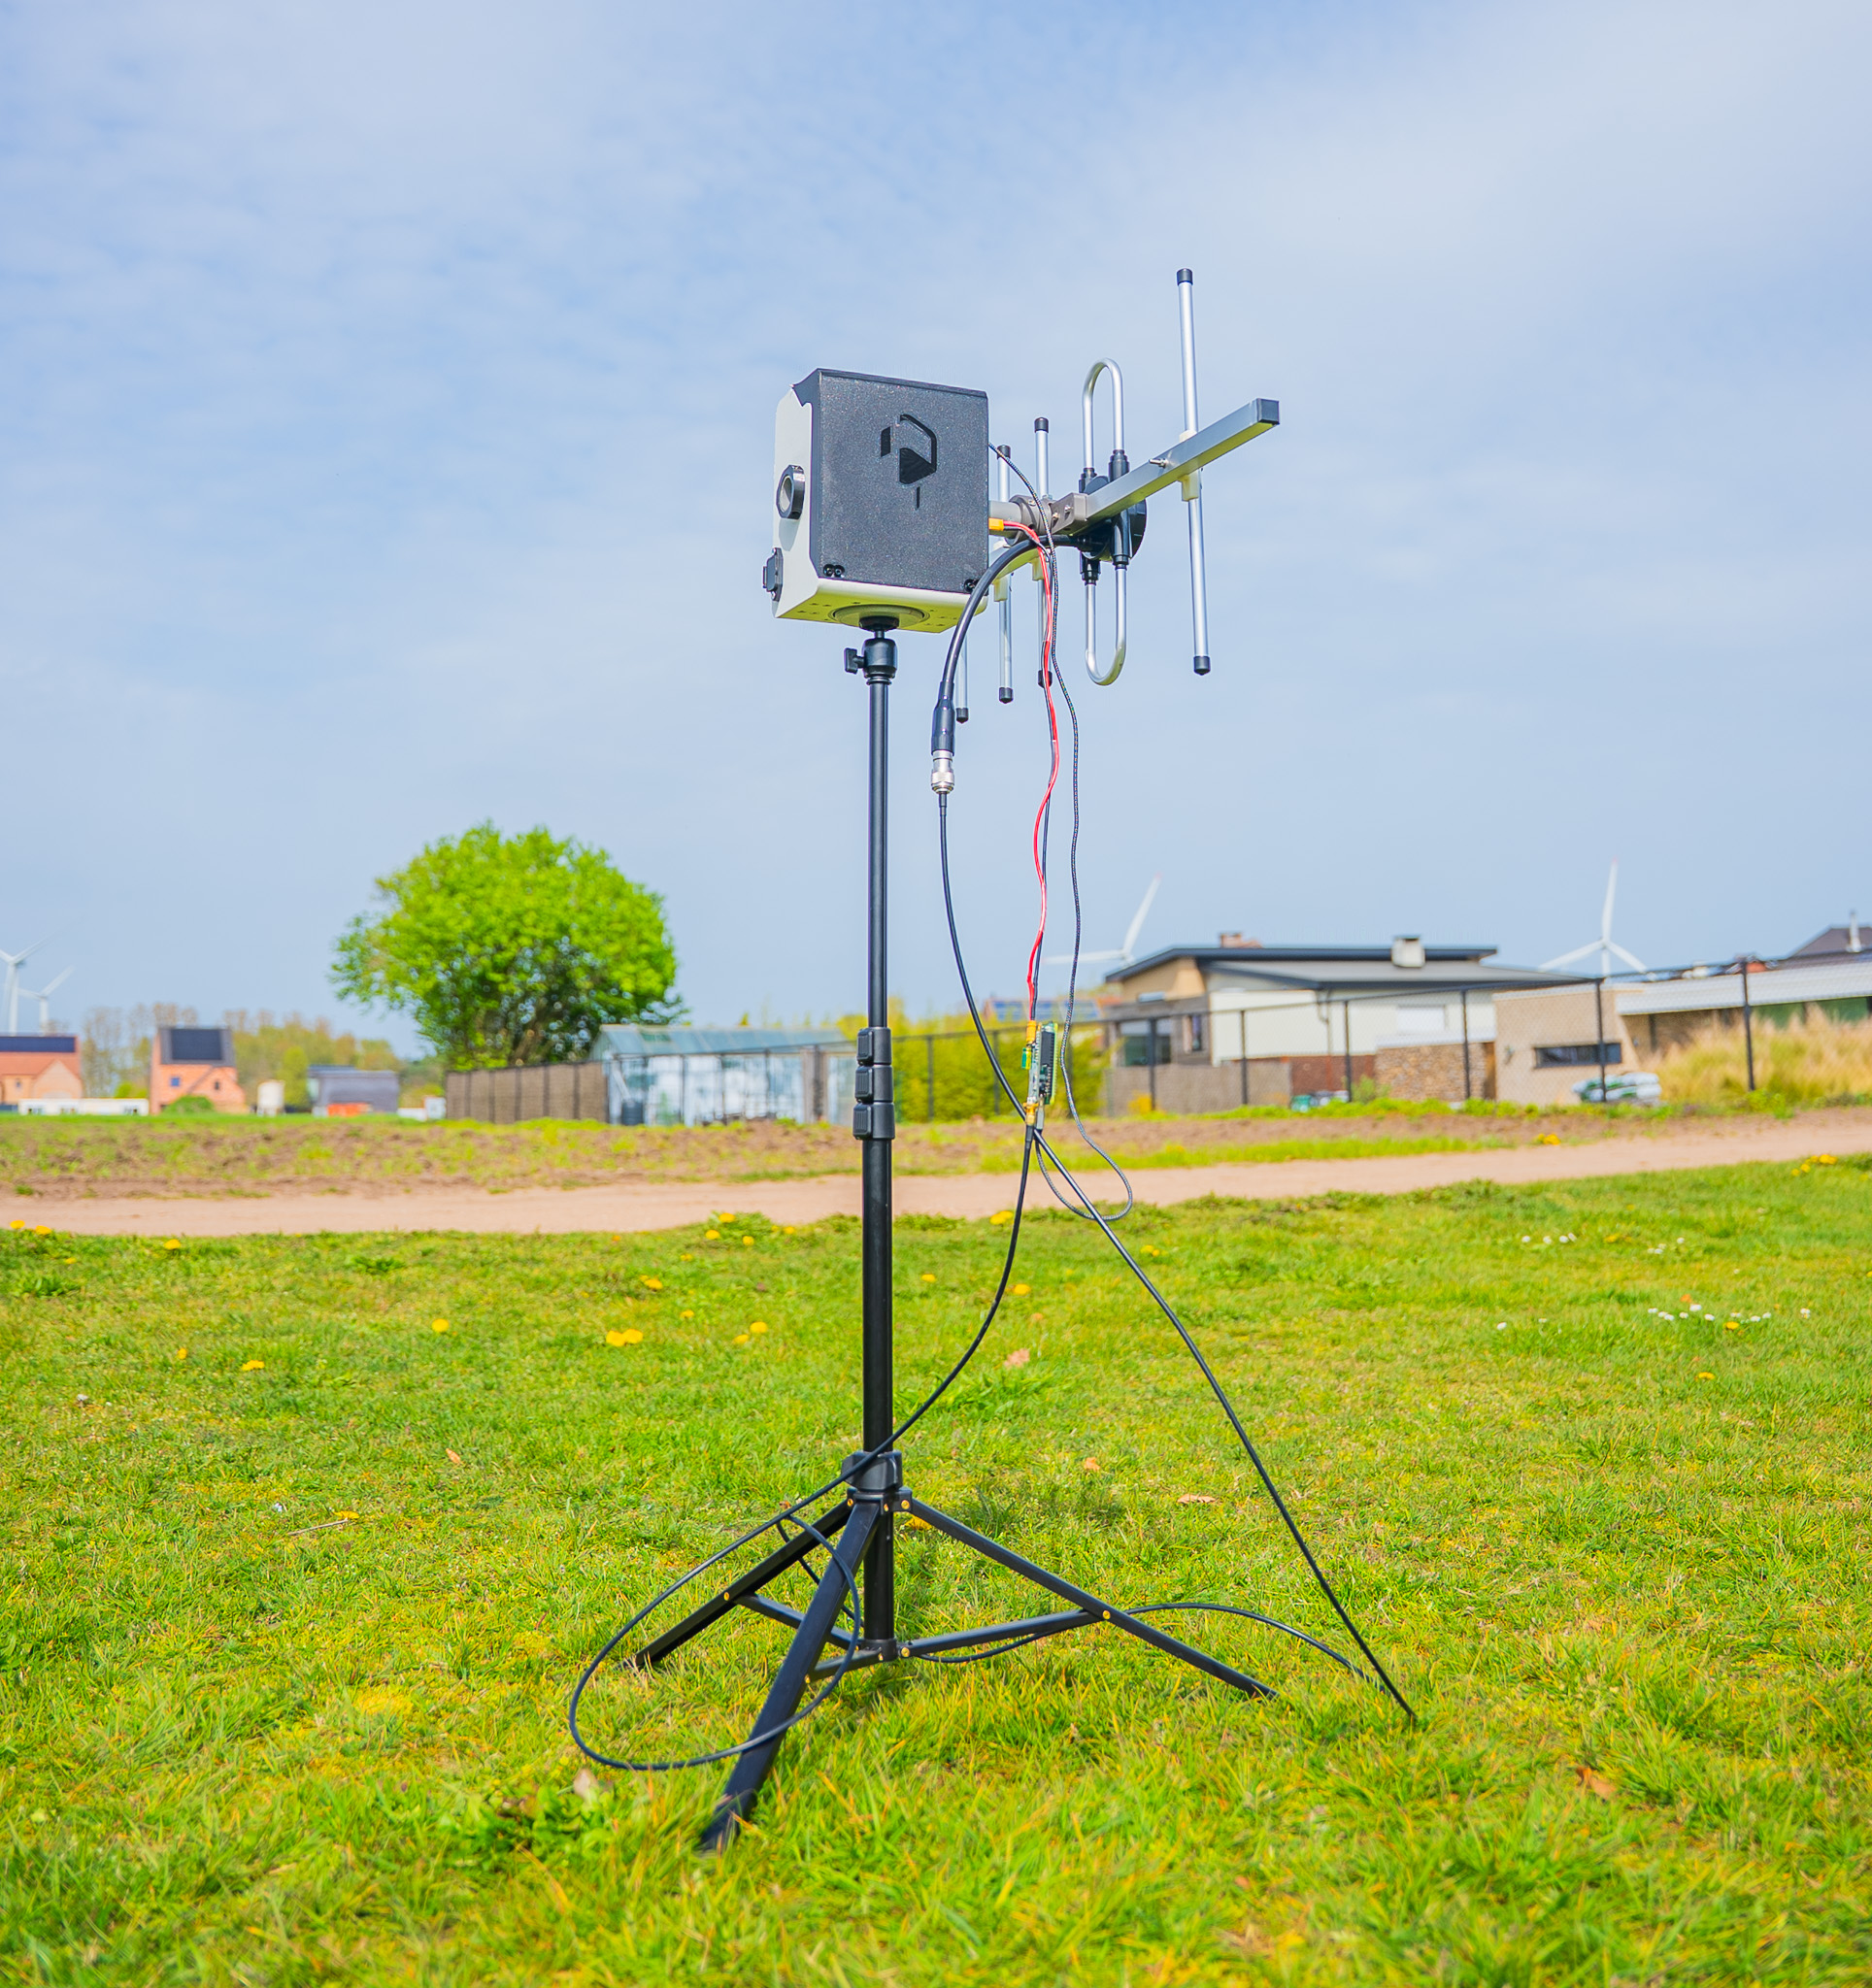
\includegraphics[width=0.75\textwidth]{photos/station_wide.jpg}
    \caption{Wide shot of the deployed station in the field.}
\end{figure}

CSV pass logs (timestamp, commanded AZ/EL, encoder AZ/EL, RSSI, frequency, Doppler offset, slant range, packet count, 5~Hz cadence) were written to \file{captures/20260409/pass\_logs/} and \file{captures/20260412/}. Across all three sessions 210 passes were logged. The Doppler correction loop ran throughout: the observed $\pm$9~kHz sweep at 432~MHz is consistent with the $\pm$11~kHz maximum predicted in \S\ref{sec:doppler}, with the commanded offset clipped at the peak radial velocity the satellite actually reaches. The noise floor and reception outcome derived from these logs are reported in \S\ref{sec:packet-reception} and are not repeated here.

\subsection{Firmware bugs surfaced by live passes}

Four firmware/software defects were diagnosed during field sessions and fixed in the same session:

\begin{itemize}
    \item AZ integral windup after zenith crossing. When the AZ axis saturated during a high-rate zenith crossing, the PID integral accumulated a large error; after the satellite descended and the rate dropped, the integral fought the proportional term and oscillated. Fixed with the saturation-based anti-windup described in \S\ref{sec:rotator-pid}: the integral stops accumulating when $|u| \geq 0.95$ and the error sign would grow it further.
    \item Duty output filter too slow. The PWM output LPF at $\alpha = 0.05$ (time constant 0.2~s) made the AZ axis unresponsive at tracking rates below $\sim$1\degree/s. $\alpha$ was raised to 0.15 (0.067~s) with no observed increase in motor-current transients; this is the deployed setting used throughout \S\ref{sec:pid-step}.
    \item Doppler base-frequency compounding. A defect in \code{set\_frequency()} overwrote the per-satellite base frequency with the Doppler-corrected value, so each successive 2~Hz update accumulated on top of the last correction. Fixed by introducing a separate \code{uhf\_base\_freq\_hz} variable that holds the satellite's nominal frequency constant across the pass, with the Doppler offset applied only when writing the CC1200 FREQ/FREQOFF registers.
    \item Rotator socket timeout. The TCP \code{set\_position()} call to \code{rotctld} blocked up to 5~s on the receive side, limiting effective tracking rate. Reduced to 0.5~s with fire-and-forget sends, plus a 15~s keepalive ping during AOS wait to keep the socket responsive. Implementation in \code{station.py}.
\end{itemize}

\section{Packet Reception: Result and Interpretation}
\label{sec:packet-reception}

As of April 2026, no protocol-valid frames have been decoded from orbit. Across the three field sessions the station tracked approximately 210 satellite passes (16 on April 1 baseline with uncalibrated RSSI readout, 184 on April 9, and 10 on April 12) and captured tens of megabytes of raw binary data, but:

No CRC-16/CCITT-valid HDLC frames (with or without G3RUH descrambling), no AX.25 frames with valid FCS, no AX.100 Mode~5 frames passing Reed--Solomon RS(255,223) correction, and consequently no decoded packets submitted to the SatNOGS DB from real satellites.

The receive chain has been validated for local test frames in a short-range ground-to-ground configuration between two devboards (\S\ref{sec:rf-measurements}): transmitted test frames decode at the receiver with valid sync word and zero payload errors across all tested frequencies, exercising the RF path, SmartRF register set, FIFO drain, and host-side decoders under those conditions. This ground validation confirms the digital and RF path is internally consistent; it does not establish that the system is receiving orbital signals.

The April 1 session predates the RSSI-readout fix (AGC\_GAIN\_ADJUST calibration) and is used as the negative control in the analysis below; the April 9 and April 12 sessions use the post-fix calibration.

\subsection{Reception Modes Deployed}

Two RX modes were used, selected per satellite by \code{station.py} (\S\ref{sec:rf-hat-firmware}):

\begin{enumerate}
    \item FIFO mode (default): CC1200 matches a sync word (e.g. AX.100 ASM \code{0x930B51DE}), then delivers fixed-length 255-byte chunks. If sync or modulation parameters don't match, the FIFO drains receiver noise after false sync triggers.
    \item Serial mode with AX.25 G3RUH decode: for $\geq$4800~bps FSK, the firmware switches to PIO serial capture and the G3RUH / NRZ-I / HDLC pipeline of \S\ref{sec:serial-mode}. No CRC-valid AX.25 frames were recovered from orbital data.
\end{enumerate}

\subsection{Why no decoded frames}

The \S\ref{sec:link-budget} link budget shows the AetherSpace downlink is already marginal at the datasheet CC1200 sensitivity ($-$5.7~dB theoretical margin at 30\degree\ elevation). In the field, board-level interference raises the effective noise floor to $-$96~dBm, burying the received signal of $-$125.7~dBm approximately 30~dB below the detection threshold. CRC-16 is error detection, not correction; RS(255,223) cannot compensate for a deficit of that size. The zero-frame outcome is the predicted outcome.

Three factors contribute:

\begin{enumerate}
    \item \textbf{Front-end noise figure and board interference.} No LNA, so the CC1200 AGC operates on antenna noise plus on-board interference (LMR51420 buck harmonics, RP2040 digital, Pi GPIO/HDMI); measured noise floor sits approximately 30~dB above the expected kTB+NF limit at the CC1200 input.
    \item \textbf{Modulation parameter uncertainty.} The SatNOGS DB does not always publish exact symbol rate / deviation / sync word for non-AetherSpace satellites; any mismatch in FIFO mode produces zero output.
    \item \textbf{Link geometry.} A +14~dBm / +2~dBi CubeSat leaves negative theoretical margin at mid-elevation even with a perfect receiver.
\end{enumerate}

\subsection{What was observed: suggestive but not diagnostic}

The captures contain statistical patterns that are individually compatible with weak sub-threshold satellite reception, but each is also compatible with receiver noise or demodulator artefacts triggered by RF activity at the sync-word matcher. Both hypotheses are named explicitly below.

\paragraph{A. Elevation-binned mean RSSI (suggestive).} Grouping 62 tracked passes by peak elevation, mean peak RSSI increases monotonically by +4.2~dB from the 0--20\degree\ bin to the 60--90\degree\ bin. Weak satellite RF entering the front end at higher elevations is one possible explanation. However, the dataset is also confounded by pointing-dependent antenna temperature, local 433~MHz interference, AGC behaviour, and pass-selection effects; a passive antenna pointed at cold sky would normally lower the noise floor relative to the horizon, so this trend cannot be treated as proof of satellite reception without calibrated controls.

\paragraph{B. Cross-capture byte matching on SNUGLITE-II (suggestive, inconclusive).} Four independent SNUGLITE-II captures contain shared subsequences up to 81 bytes long. Two hypotheses are compatible: (i) repeated beacon frames captured at different orbital points, and (ii) a CC1200 demodulator/idle pattern emitted repeatedly at false sync triggers. The April 9 log explicitly identifies a 99-byte CC1200 idle pattern appearing identically across all satellites at all frequencies; the SNUGLITE-II matches have not yet been shown to differ structurally from this idle pattern, so (ii) is not excluded.

\paragraph{C. Pass-profile RSSI range (weak).} A small subset of passes show an AOS-to-peak-to-LOS RSSI excursion of several dB, loosely consistent with $1/r^2$ path-loss modulation of a real signal but equally consistent with antenna noise-temperature variation as the beam sweeps across ground and sky. Not diagnostic.

\begin{figure}[H]
    \centering
    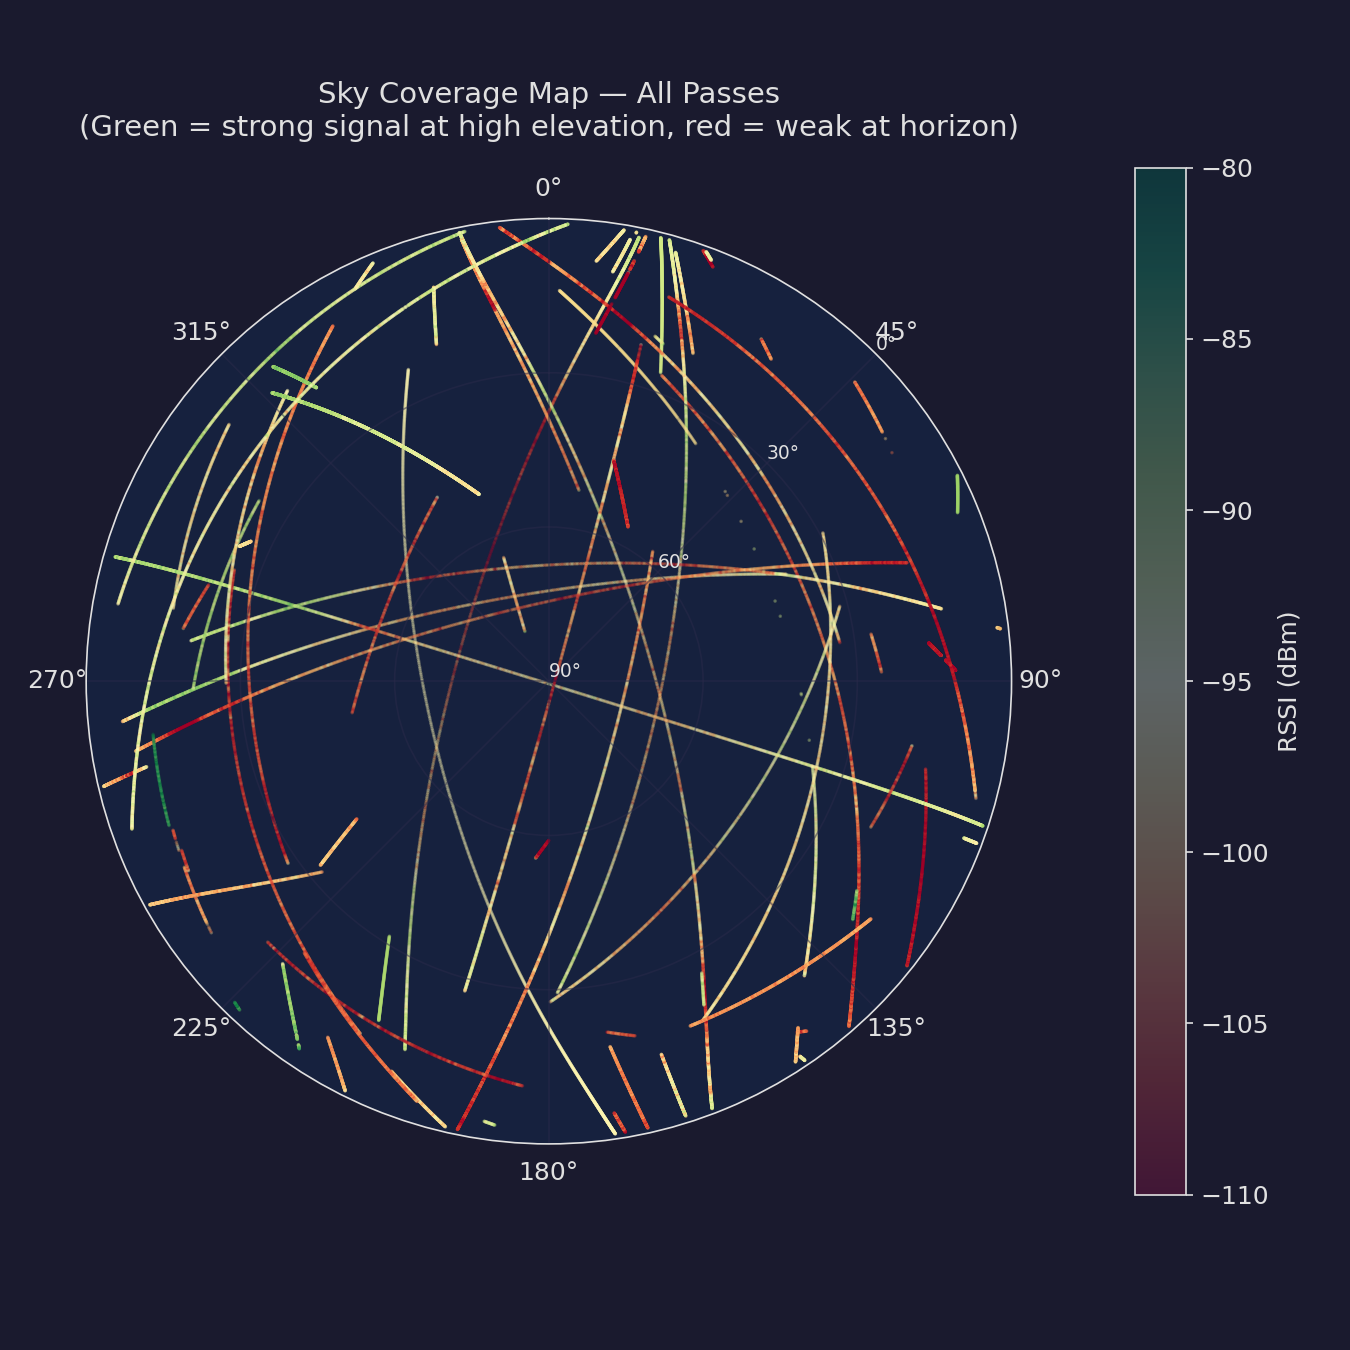
\includegraphics[width=0.8\textwidth]{figures/evidence/10_sky_coverage.png}
    \caption{Sky coverage heatmap: RSSI over AZ/EL across all tracked passes.}
\end{figure}

\paragraph{D. Doppler-sweep profile (confirms orbital geometry, not reception).} The expected $\pm$9~kHz sweep at 432~MHz with zero-crossing at TCA is observed on every pass. Because this sweep is \textit{applied} by station software to the FREQOFF register regardless of whether any signal is present, it verifies correct predict/correct software behaviour only.

\begin{figure}[H]
    \centering
    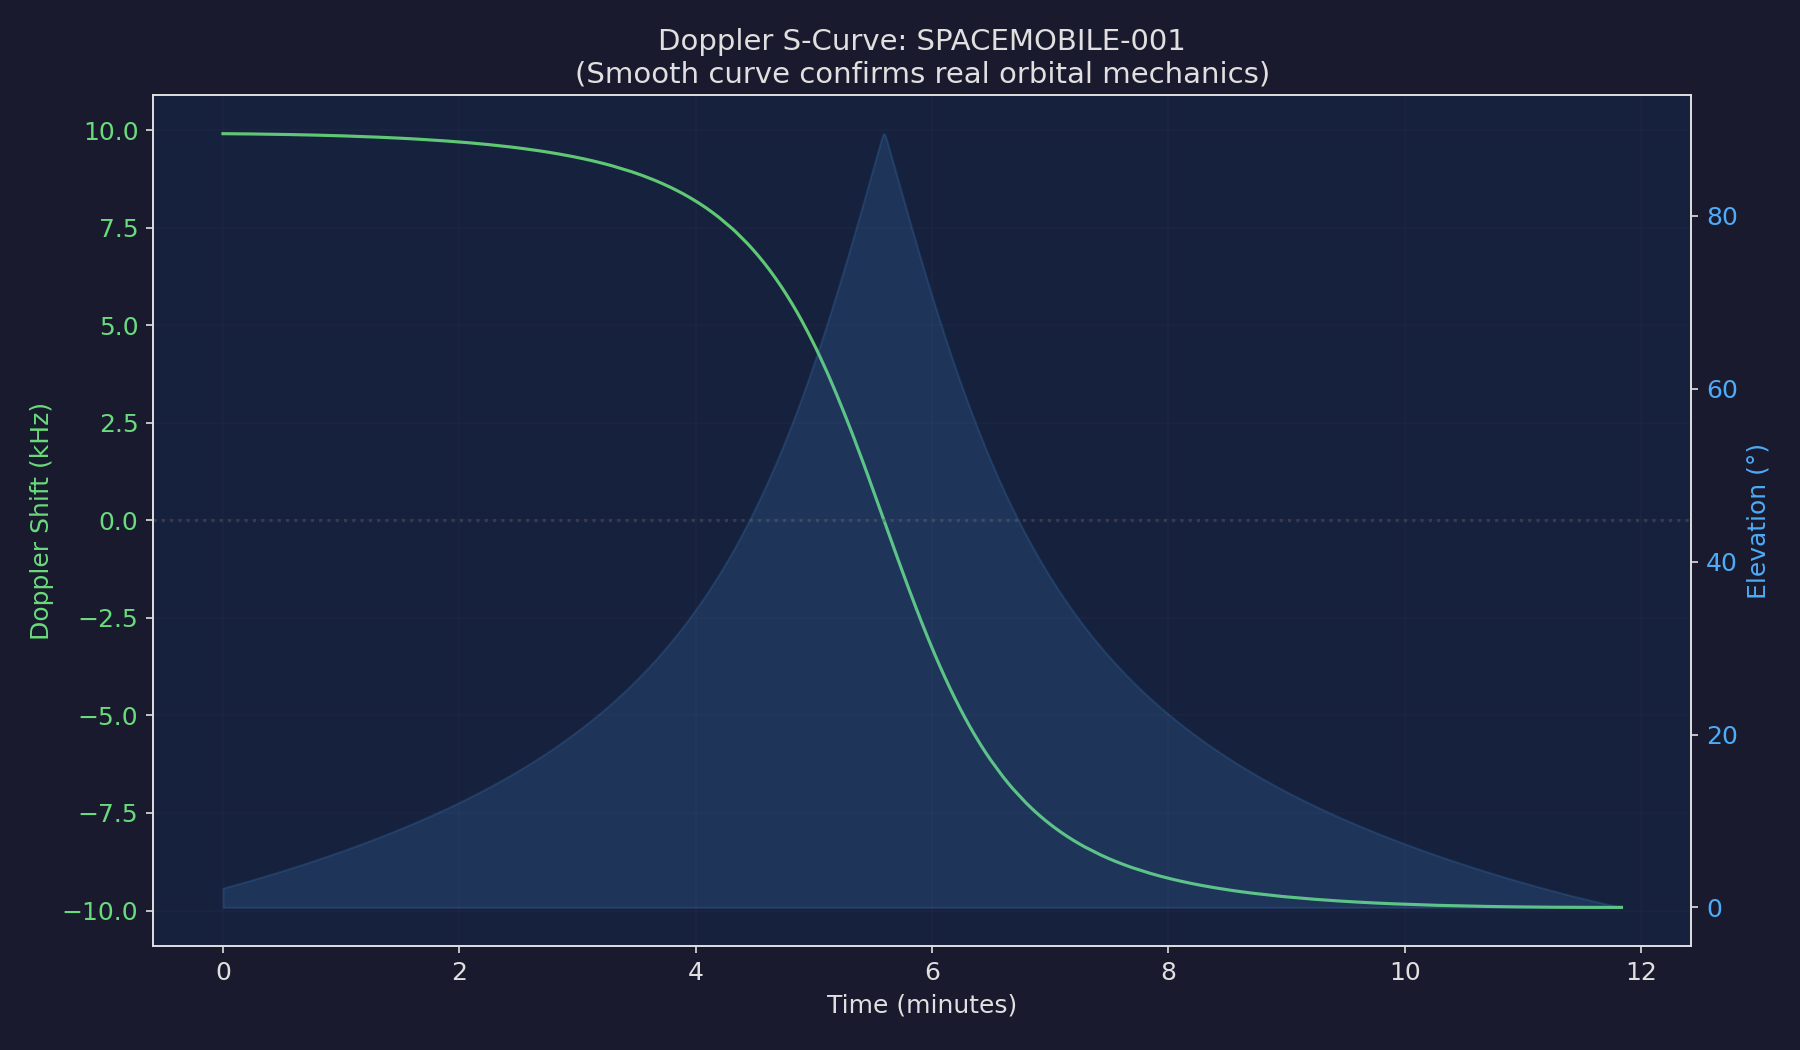
\includegraphics[width=0.8\textwidth]{figures/evidence/06_doppler_scurve.png}
    \caption{Doppler-correction S-curve applied during one pass.}
\end{figure}

\paragraph{E. Capture-byte entropy (weak).} Captures show byte entropy of 6.95--7.91 bits/byte, below the 8.0 bits/byte expected of uniform random noise. Filtered or correlated noise from a demodulator can produce similar signatures without encoding any information. The entropy is consistent with ``not white noise'' but not with ``structured satellite telemetry'' specifically.

\paragraph{F. MIMAN AX.100 Mode~5 analysis (inconclusive).} MIMAN captures processed through AX.100 Mode~5 achieved Golay(24,12) decode rates of 73\,\% (April 9) and 66\,\% (April 12). The random false-positive baseline for Golay(24,12) with 3-error correction is approximately 57\,\%, so the observed rates are only marginally above chance. Zero frames passed the subsequent RS(255,223) correction. Golay matches without downstream RS-decoded content are not a definitive indicator. See \file{captures/evidence/miman\_decode\_report.json}.

\subsection{Academic Conclusion}

The primary finding is established independently of observations A--F: the theoretical margin at 30\degree\ elevation is already $-$5.7~dB at datasheet CC1200 sensitivity, and the field-measured noise floor of $-$96~dBm buries the $-$125.7~dBm received signal by approximately 30~dB, making protocol-valid decode physically impossible regardless of which secondary hypothesis explains the statistical patterns. The secondary finding is that A--F are individually consistent with both weak sub-threshold reception and receiver-internal noise artefacts, and cannot be used to distinguish between the two hypotheses. This ambiguity is expected and does not alter the root-cause diagnosis: the board-noise floor sits approximately 30~dB above the thermal\,+\,NF baseline. A mast-mounted front-end LNA is the primary intervention: its gain lifts the received signal above the fixed board-interference floor before it reaches the CC1200. However, with the field noise floor at $-$96~dBm, a 20~dB LNA still leaves the signal approximately 10~dB below the detection threshold, so the LNA must be combined with board-level EMI mitigation: improved buck-converter output filtering, a post-buck LDO on the CC1200 supply rails to suppress conducted switching noise, and a SAW bandpass filter on the antenna port to reject out-of-band interference before it reaches the LNA (\S\ref{sec:future-work}).

\subsection{AetherSpace-Specific Outlook}

For AetherSpace the modulation-match risk is lower than for arbitrary satellites because the CubeSat and the ground station use the same CC1200 transceiver, provided both sides load the same finalised SmartRF register set. The remaining risk is sensitivity, addressed in \S\ref{sec:future-work}. The software architecture already exposes an \code{RfBackend} abstraction with both CC1200 and RTL-SDR implementations, allowing an SDR-based wideband IQ capture to serve as an independent verification path once an LNA is installed.

\section{Cost Comparison}

The v2 MOTOR\_RF\_HAT BOM (from \S\ref{sec:cost}) compared against commercial and existing open-source alternatives. The ``rotator'' column counts the controller board + motors + mechanics only, excluding the station computer, antenna, coax, power supply, and tripod; ``total'' adds a Pi 3A+.

\begin{table}[H]
    \centering
    \small
    \begin{tabular}{@{}llll@{}}
        \toprule
        System & Type & Rotator (\euro{}) & +Pi (\euro{}) \\
        \midrule
        Yaesu G-5500   & Commercial    & 760--900   & 1200+ \\
        SPID RAS       & Commercial    & 1200--1300 & 1800+ \\
        SatNOGS v3     & Stepper, belt & 300--500   & 600+ \\
        \textbf{This work (v2)} & \textbf{DC + gears} & \textbf{$\sim$75} & \textbf{$\sim$100} \\
        \bottomrule
    \end{tabular}
    \caption{Cost comparison. v2 is design-complete but not yet fabricated; $\sim$\euro{}75/\euro{}100 are BOM projections (LCSC + JLCPCB, April 2026).}
\end{table}

% ══════════════════════════════════════════════════════════════════════════════
\chapter{Conclusion and Future Work}
\label{ch:conclusion}
% ══════════════════════════════════════════════════════════════════════════════

\section{Research Questions Answered}

\textbf{Main research question.} Can an economical, portable SatNOGS-compatible ground station be designed, built, and field-validated as the ground segment for the AetherSpace CubeSat mission? \textbf{Yes, with one open item.} The station was designed, fabricated, and field-deployed across three sessions totalling approximately 210 tracked passes. The rotator meets its pointing requirements, the RF chain is end-to-end verified in ground-to-ground tests, SatNOGS network integration is in place via EasyComm III and SiDS, and the station deploys in approximately four minutes from a camera tripod. The single open item is orbital frame reception: no protocol-valid frames were decoded from orbit, with the root cause identified as a missing front-end LNA. The hardware change required to close the sensitivity gap is specified in \S\ref{sec:future-work}; once applied, the station is ready to receive AetherSpace telemetry when the satellite launches.

\begin{enumerate}
    \item Under €50 rotator / €100 station? Partially. v2 (\S\ref{sec:cost}) reaches $\sim$€40 for the combined controller/RF PCB, $\sim$€75 for the full rotator hardware, and $\sim$€100 for the station core (excluding antenna, coax, power supply, tripod). The strict ``full rotator under €50'' target is not met once motors and mechanics are included. The v1 setup used for field validation costs $\sim$€145 (two separate boards, 6-layer RF HAT).
    \item Pointing accuracy? Measured: $<$0.5\degree\ EL and 0\degree--3\degree\ AZ in the 20\degree--70\degree\ peak-elevation band (\S\ref{sec:tracking-accuracy}). Encoder resolution 0.00409\degree\ AZ, 0.00793\degree\ EL (\S\ref{sec:gearing}). Both axes stay inside the Siretta Oscar 44 3-dB beamwidths (54\degree\ H, 48\degree\ E). The large AZ excursions at $>$70\degree\ elevation are a motor-speed-limit event, not a control-loop accuracy limit.
    \item SatNOGS integration? Yes on the rotator side via standard EasyComm III / hamlib model 204, and on the telemetry side via SiDS (station 4712 registered). The CC1200 is incompatible with the SDR-based \code{satnogs-client}, so the station does not appear ``online'' on the observation-scheduling map; this is a deliberate choice, not a defect.
    \item DC vs stepper? DC motors were chosen (rationale in \S\ref{sec:motors}). Empirical results: zero motor current draw when stationary, $<$0.5\degree\ EL / 0\degree--3\degree\ AZ tracking in the link-closing elevation band, 35\degree/s peak slew at 95\,\% duty. Cost: 100~Hz PID with quadrature decode, running within the RP2040 timing budget (ISR latency $<$10~$\mu$s; inter-edge period 117~$\mu$s at 35\degree/s).
    \item CC1200 sensitivity? The assembled RF HAT achieves approximately $-$105~dBm in bench conditions and $-$96~dBm outdoors (\S\ref{sec:packet-reception}). The dominant limiting factor is board-level interference: LMR51420 buck-converter harmonics, RP2040 digital noise, and Pi GPIO emissions lift the effective noise floor approximately 30~dB above the thermal\,+\,NF baseline, degrading sensitivity from the datasheet $-$120~dBm to approximately $-$105~dBm and leaving the AetherSpace link at $-$20.7~dB measured margin at 30\degree\ elevation. A mast-mounted LNA is the single hardware change required to recover the lost margin (\S\ref{sec:future-work}).
    \item CC1200 vs SDR? For AetherSpace specifically, the CC1200 approach is the better fit: both ends use the same transceiver, so a single SmartRF register set loaded at both ends eliminates modulation-parameter uncertainty. The trade-off is reduced flexibility for other satellites and incompatibility with the standard \code{satnogs-client} pipeline. The sensitivity gap documented in Q5 is not inherent to the CC1200 approach; it is a board-interference problem that an LNA would resolve equally for any narrow-band receiver on this hardware.
\end{enumerate}

\section{Limitations}

\begin{itemize}
    \item No protocol-valid frames decoded from orbit: documented in \S\ref{sec:packet-reception} with per-observation alternative hypotheses; root cause identified in \S\ref{sec:link-budget} and \S\ref{sec:field-tests} as the absence of an external LNA combined with a board-noise floor approximately 30~dB above the expected kTB+NF limit, degrading effective CC1200 sensitivity from the datasheet $-$120~dBm to approximately $-$105~dBm and leaving the AetherSpace link at approximately $-$20~dB measured margin at 30\degree\ elevation (best case; typical outdoor conditions are worse).
    \item No calibrated-source RF verification against a signal generator. Sensitivity has been validated in relative terms (ground-to-ground CC1200-to-CC1200 decode, \S\ref{sec:packet-reception}) but not against a signal generator injecting a known power level into the SMA. A sig-gen sweep would separate ``receive chain works but insensitive'' from ``receive chain has an undiagnosed defect'' independently of link geometry.
    \item VHF path not validated. The 144/145~MHz front-end is routed on the RF HAT but not populated. It would need a VNA-based matching-network tune before uplink use.
    \item Zenith AZ rate saturation. The motor's 35\degree/s ceiling is exceeded briefly during high-elevation passes (near-zenith passes can demand $>$10\degree/s of \textit{azimuth} rate for a few seconds, even though the total angular rate never exceeds $\sim$1.1\degree/s). The AZ axis saturates during this window and recovers as the satellite descends below $\sim$70\degree\ elevation.
    \item First-rev PCB issues: bodge wires (AZ IN1 rerouted GP15$\to$GP16), replaced TB6642FG, removed encoder RC caps. All addressed in the v2 MOTOR\_RF\_HAT design.
    \item Design-complete v2 not yet built. The cost claim relies on v2 BOM pricing; v2 has not been fabricated in time for this thesis. The v2 design incorporates every lesson from v1 bring-up and is ready to order.
\end{itemize}

\section{Future Work}
\label{sec:future-work}

\begin{enumerate}
    \item Build the v2 MOTOR\_RF\_HAT: fabricate and assemble the design-complete combined board. Validates the $\sim$€100 station-core cost projection end-to-end and removes the v1 bodges.
    \item External mast-mounted LNA: the single most impactful reception change. Concrete recommendation:
    \begin{itemize}
        \item LNA: Qorvo QPL9547 (NF $\sim$0.3~dB, $\sim$20~dB gain at 433~MHz, +5~V) as a modern replacement for the discontinued SPF5189Z. Mini-Circuits PGA-103+ (NF $\sim$0.6~dB, $\sim$20~dB gain at 433~MHz) is an equivalent in-stock part. There is no TI companion LNA for this band; the CC1190 range extender covers 850--950~MHz only.
        \item SAW pre-filter (optional but recommended): 433.92~MHz SAW bandpass before the LNA, to reject out-of-band ISM / PMR / ATV interferers that otherwise compress the LNA and lift the AGC.
        \item Architecture: mast-mount the LNA, fed over the antenna SMA coax via a bias-T on the RF HAT (a 470~nH--1~$\mu$H RF choke plus DC-block capacitor; the choke reactance must be well above $Z_0 = 50~\Omega$ at 433~MHz to keep insertion loss negligible: 470~nH gives $X_L \approx 1.3~\text{k}\Omega$, yielding ${\approx}$0.2~dB loss; 120~nH gives only 326~$\Omega$ and ${\approx}$0.6~dB, which is significant ahead of a low-noise amplifier). Placing the LNA at the antenna feed rather than after the coax makes the LNA's NF set the whole-chain NF (Friis cascade) and pre-amplifies before the 0.5--1~dB RG-58 loss and the 15--20~dB board-noise elevation measured on v1.
        \item Antenna (optional secondary upgrade): a 10--12~dBi Yagi in place of the Oscar~44 adds a few dB, but the dominant gap is the LNA and the antenna upgrade is not required to close the link.
    \end{itemize}
    Combined impact (LNA alone, existing Yagi): system NF $\sim$7~dB $\to$ $<$1~dB, AGC lifts off the board-noise floor. Effective sensitivity improves by 15--20~dB, moving the AetherSpace link at 30\degree\ elevation from $-$20.7~dB measured to roughly 0\ldots$+$5~dB. v2 PCB change: add a bias-T network on the UHF SMA port; the LNA itself stays off-board.
    \item AetherSpace integration: once AetherSpace's final packet format is published, load the matching SmartRF profile. A CC1200-to-CC1200 link removes a large part of the modulation-parameter uncertainty if both ends use the same register profile; the open question is sensitivity, addressed by (2).
    \item RTL-SDR hybrid: add an RTL-SDR for wideband IQ capture and visual waterfall. Useful as an independent verification path for CC1200 reception claims. Software architecture already supports it via the abstract \code{RfBackend} interface.
    \item VHF uplink: populate the 144/145~MHz matching network, VNA-tune, and enable uplink commanding once AetherSpace defines an uplink protocol.
    \item Battery field test: validate the 20--28~h runtime projection with current measurements at each operating point on a representative 6S pack.
\end{enumerate}

\section{Summary}

This thesis designs, builds, and partially validates a portable SatNOGS-compatible ground station. The v1 hardware (two separate boards, used in the field sessions) tracks satellites with sub-0.5\degree\ elevation error and 0\degree--3\degree\ azimuth error in the 20\degree--70\degree\ peak-elevation band, integrates with the SatNOGS rotator ecosystem through standard EasyComm III, and deploys from unpacked to tracking in about four minutes using only a laptop (a phone can also supply GPS in a pinch). The v2 MOTOR\_RF\_HAT (design-complete, unfabricated at submission) projects to $\sim$€40 for the combined controller/RF PCB and $\sim$€100 for the station core; the projection remains to be validated by fabrication.

The main open gap is reception. No protocol-valid frames were decoded from orbit across approximately 210 tracked passes; the root cause is documented in \S\ref{sec:packet-reception} and \S\ref{sec:link-budget} as the absence of an external LNA combined with a measured board-noise floor approximately 30~dB above the thermal+NF limit, and the mitigation is specified in \S\ref{sec:future-work} item 2.

The concrete deliverables of this thesis are: (a)~a built and field-validated 3D-printed AZ/EL rotator, (b)~custom RP2040 motor-controller firmware with closed-loop PID, IMU-based homing, and runaway safety, (c)~a dual-CC1200 Raspberry Pi HAT with a design-complete combined v2 variant consolidating motor control and RF front-end onto one 6-layer board, (d)~a $\sim$7\,900 LOC Python stack covering pass prediction, Doppler correction, per-pass CC1200 reconfiguration, and SatNOGS DB telemetry submission, (e)~a zero-SSH laptop-based field-deployment workflow, and (f)~a first-principles and measurement-grounded link-budget analysis that quantifies the sensitivity gap blocking orbital decode and names the specific front-end change (LNA) that would close it. The 2023 KU~Leuven masterproef by Hanssens~\cite{hanssens2023} provided the survey of the SatNOGS ecosystem and the torque-deficit finding that motivated the DC-motor path, and is referenced throughout this thesis as background rather than as a benchmark to compete with.


% Bibliography
\printbibliography

% Appendices
\appendix
% ══════════════════════════════════════════════════════════════════════════════
\chapter{GPIO Pin Mapping}
\label{app:pinout}
% ══════════════════════════════════════════════════════════════════════════════

% ══════════════════════════════════════════════════════════════════════════════
\chapter{EasyComm Command Reference}
\label{app:protocol}
% ══════════════════════════════════════════════════════════════════════════════

% ══════════════════════════════════════════════════════════════════════════════
\chapter{PID Tuning Constants}
\label{app:pid}
% ══════════════════════════════════════════════════════════════════════════════

% ══════════════════════════════════════════════════════════════════════════════
\chapter{Detailed Bill of Materials}
\label{app:bom}
% ══════════════════════════════════════════════════════════════════════════════

The BOM below costs the \textbf{v2 combined MOTOR\_RF\_HAT} (design-complete, routed, ready to order, not yet fabricated at the time of submission). Field validation used the v1 two-board setup (separate MotorPCB + RF HAT), which was more expensive because each board was ordered separately and the RF HAT uses a 6-layer stackup. The lessons from v1 bring-up (\S\ref{sec:bringup}) are incorporated into the v2 BOM: A4950 replaces TB6642FG for availability, and four 100\,$\Omega$ series resistors (R11--R14) protect the A4950 logic inputs from GPIO transients. The off-board rotator BOM (motors, gears, bearings, chassis, fasteners) is unchanged from v1.

Component prices from the LCSC BOM tool (April 2026), hand-assembled. Full machine-readable BOM in \file{ThesisPaper/bom\_complete.csv}.

\section*{D.1 \ MOTOR\_RF\_HAT PCB --- on-board components}

125 placed components (excluding test pads and mounting holes), 48 unique LCSC line items.

\begin{table}[H]
    \centering
    \begin{tabularx}{\textwidth}{lXrr}
        \toprule
        Category & Key components & Qty & LCSC total (\euro{}) \\
        \midrule
        Capacitors & 19 values (0603/0805/1206), CC1200 matching + bypass & 71 & 7.41 \\
        Inductors & 11 values (0603 RF + 3030 power), CC1200 matching & 17 & 1.18 \\
        Resistors & 7 values (0603) & 14 & 0.07 \\
        CC1200RHBR & UHF + VHF transceivers (C122881) & 2 & 4.43 \\
        A4950ELJTR-T & Motor drivers AZ + EL (C82404) & 2 & 1.10 \\
        LMR51420YFDDCR & 24~V $\to$ 5~V buck (C7296200) & 1 & 0.84 \\
        WS2812B-2020 & Status LEDs (C965555) & 4 & 0.28 \\
        40~MHz crystal & CC1200 reference (C5380316) & 2 & 0.12 \\
        BSS138 & Level shifter (C112239) & 1 & 0.01 \\
        1N4148WS & Protection diode (C2128) & 1 & 0.01 \\
        D\_Schottky & Buck diode (C3759853) & 1 & 0.14 \\
        XT30PW-M & 24~V power input (C431092) & 1 & 0.24 \\
        2$\times$20 Pi header & GPIO (C50980) & 1 & 0.14 \\
        JST XH 6-pin & Motor/encoder connectors (C157919) & 2 & 0.33 \\
        \midrule
        Visible line-item sum & & & 16.30 \\
        MOQ rounding uplift & (reels of 100 for 1--8-piece needs) & & 12.14 \\
        \textbf{LCSC subtotal} & & & \textbf{28.44} \\
        \bottomrule
    \end{tabularx}
    \caption{MOTOR\_RF\_HAT on-board component cost breakdown.}
\end{table}

Items sourced outside the default LCSC reflow batch (hand-soldered or not stocked at LCSC):

\begin{table}[H]
    \centering
    \begin{tabular}{llrr}
        \toprule
        Component & LCSC~\# & Qty & \euro{} \\
        \midrule
        SMA edge-mount connector & (not on LCSC) & 2 & 1.50 \\
        15~nH 0603 inductor & C23651 & 2 & 0.50 \\
        Raspberry Pi Pico (hand-soldered) & C7203002 & 1 & 4.00 \\
        \midrule
        \textbf{Subtotal} & & & \textbf{6.00} \\
        \bottomrule
    \end{tabular}
    \caption{Hand-soldered / off-batch items.}
\end{table}

\section*{D.2 \ PCB fabrication}

\begin{table}[H]
    \centering
    \begin{tabular}{lr}
        \toprule
        Item & \euro{} \\
        \midrule
        Bare PCB (6-layer, JLCPCB, per board from 5-piece order) & 6.00 \\
        \bottomrule
    \end{tabular}
    \caption{PCB fabrication cost (per board).}
\end{table}

\section*{D.3 \ Off-board components}

\begin{table}[H]
    \centering
    \begin{tabular}{llrr}
        \toprule
        Component & Source & Qty & \euro{} \\
        \midrule
        FAPG36-555-EN motor (24~V, 516:1) & AliExpress & 2 & 16.00 (line) \\
        Raspberry Pi 3 Model A+ & RPi distributor & 1 & 25.00 \\
        ASA filament ($\sim$400~g) & local & 1 & 10.00 \\
        Steel balls 3~mm (50~pcs) & AliExpress & 1 & 2.00 \\
        M4$\times$10 + M3$\times$8 screws, heat-set inserts & local & lot & 3.00 \\
        PVC pipe + misc hardware & local & lot & 2.00 \\
        ADXL345 IMU breakout & AliExpress & 1 & 1.50 \\
        \midrule
        \textbf{Off-board subtotal} & & & \textbf{59.50} \\
        \bottomrule
    \end{tabular}
    \caption{Off-board mechanical and computing components.}
\end{table}

\section*{D.4 \ Grand total}

\begin{table}[H]
    \centering
    \begin{tabular}{lr}
        \toprule
        Subsystem & \euro{} \\
        \midrule
        MOTOR\_RF\_HAT components (LCSC) & 28.44 \\
        Hand-soldered parts (SMA, 15~nH, Pico) & 6.00 \\
        Bare PCB (6-layer) & 6.00 \\
        Off-board components & 59.50 \\
        \midrule
        \textbf{Grand total per station core} & \textbf{$\sim$€100} \\
        \bottomrule
    \end{tabular}
    \caption{v2 grand-total cost (station core, excluding antenna, coax, power supply, and tripod).}
\end{table}

Excludes antenna, coax cable, 24~V power supply, and tripod (user-supplied). Hand-assembled, so no JLCPCB PCBA fees. LCSC total includes MOQ rounding (buying 100 passives when 1--8 are needed). The combined MOTOR\_RF\_HAT board eliminates the separate motor controller PCB and USB cable between Pi and rotator used in v1 testing. Numbers are projections for the unfabricated v2 board.


% Code of Conduct (GenAI) — mandatory
\input{code-of-conduct}

\end{document}
